\documentclass[letterpaper,twocolumn,10pt]{article}
% Official USENIX style (OSDI '27): 7" x 9" text block, two columns,
% 10pt Times on 12pt leading. Do not change margins, fonts, or spacing.
\usepackage{usenix-2020-09}

\usepackage{tikz}
\usetikzlibrary{arrows.meta, positioning, fit, calc, backgrounds}
\usepackage{graphicx}
\usepackage{booktabs}
\usepackage{longtable}
\usepackage{pdflscape}
\usepackage{multirow}
\usepackage{subcaption}
\usepackage{amsmath,amssymb}
\usepackage{mathtools}
\usepackage{xspace}
\usepackage{hyphenat}
\usepackage{enumitem}
\usepackage{tabularx,array}
\usepackage{xurl}
\usepackage[normalem]{ulem}
\usepackage{listings}
\lstset{basicstyle=\ttfamily\scriptsize, columns=fullflexible, keepspaces=true, breaklines=true}
% Numbered citations, as in the USENIX sample paper. plainnat keeps the URLs of
% web-only references, which the plain style would drop. natbib prints one
% harmless warning about the cite package that the USENIX style loads.
\usepackage[numbers,sort&compress]{natbib}
\usepackage{algorithm}
\usepackage{algorithmic}
\providecommand{\theHalgorithm}{\arabic{algorithm}}

% ---------------------------------------------------------------------------
% Build switch.
%   \appendixfalse : OSDI submission PDF = paper + references only.
%                    The 12-page limit covers everything except references,
%                    so the appendix cannot ride along in this PDF.
%   \appendixtrue  : full internal draft, appendix attached after references.
% The supplement PDF for upload is built from appendix.tex.
% ---------------------------------------------------------------------------
\newif\ifappendix
\appendixfalse
%\appendixtrue

\usepackage{siunitx}
\usepackage{colortbl}
\usepackage{xspace}

\newcommand\accnum[1]{\num[round-precision=3]{#1}}
\newcommand\pernum[1]{\num[round-precision=1]{#1}}
\newcommand\scnum[1]{\num[scientific-notation=true,round-precision=1]{#1}}
\newcommand\numt[1]{\num[round-precision=2,round-mode=figures,scientific-notation=true]{#1}}
\newcommand\numo[1]{\num[round-precision=1,round-mode=figures,scientific-notation=true]{#1}}
%\newcommand{\numo}[1]{
%\pgfmathparse{#1}\pgfmathprintnumberto[precision=1, assume math mode=true]{\pgfmathresult}{\roundednumber}\roundednumber
%}
%\newcommand{\numt}[1]{
%\pgfmathparse{#1}\pgfmathprintnumberto[precision=2, assume math mode=true]{\pgfmathresult}{\roundednumber}\roundednumber
%}

\newcommand{\pref}[1]{page~\pageref{#1}}
\newcommand{\vect}[1]{\boldsymbol{#1}} % vector
\newcommand{\mat}[1]{\boldsymbol{#1}}  % matrix
\newcommand{\defeq}{\ensuremath{\mathrel{\mathop:}=}}
\newcommand{\eqdef}{\ensuremath{=\mathrel{\mathop:}}}

% \newcommand{\ipoint}[1]{\textit{\textbf{\color{darkgray}#1}}}
\newcommand{\ipoint}[1]{\textit{\textbf{\color{black!60}#1}}}
\newcommand{\todo}[1]{{\color{red}\textit{TODO}: #1}}
%\newcommand{\comment}[1]{{\color{blue}comment: #1}}
\newcommand{\commentout}[1]{}
\renewcommand{\b}[1]{{#1}}
\newcommand{\grbf}[1]{\mbox{\boldmath${#1}$\unboldmath}} %\renewcommand{\grbf}[1] {\mathbf{#1}}
\newcommand{\ns}[1]{\ensuremath{\mathbb{#1}}}
\newcommand{\fs}[1]{\ensuremath{\mathcal{#1}}}
\newcommand{\idiv}{\ensuremath{\nabla\cdot}}
\newcommand{\igrad}{\ensuremath{\nabla}}
\newcommand{\ilap}{\rotatebox[origin=c]{180}{$\nabla$}}
\newcommand{\icurl}{\ensuremath{\nabla \times}}
\newcommand{\tr}{\ensuremath{\operatorname{tr}}}
\newcommand{\id}{\ensuremath{\operatorname{id}}}
\newcommand{\ts}{\textsuperscript}
\newcommand{\half}[1]{\frac{#1}{2}}
\renewcommand{\d}[1]{\mathop{}\!\mathrm{d}#1}
\newcommand{\dt}{\d{t}}
\newcommand{\dx}{\d{\vect{x}}}
\newcommand{\op}[1]{\ensuremath{\mathcal{#1}}}
\newcommand{\di}[1]{\ensuremath{\mathbf{#1}}}


\newcommand{\MA}[1]{{\mathcal #1}}
\newcommand{\reals}{\mathbb{R}}
\newcommand{\codenm}[1]{{\tt  #1}}
\newcommand{\zapspace}{\topsep=0pt\partopsep=0pt\itemsep=0pt\parskip=0pt}

\newcommand{\msection}[1]{\section{#1}}
\newcommand{\msubsection}[1]{\subsection{#1}}
%\newcommand{\msection}[1]{\section{#1}}
%\newcommand{\msubsection}[1]{\subsection{#1}}


\definecolor{light-gray}{gray}{0.80}
%\renewcommand{\algorithmiccomment}[1]{#1}


\newcommand{\mcol}[2]{\multicolumn{#1}{r}{#2}}
\newcommand{\mrow}[2]{\multirow{#1}{*}{#2}}
\newcommand{\mrowrot}[2]{
\parbox[t]{2mm}{\multirow{#1}{*}{\rotatebox[origin=c]{90}{#2}}}
}


%\newcommand{\algcolor}[2]{\hspace*{-\fboxsep}\colorbox{#1}{\parbox{\linewidth}{#2}}}
\newcommand{\algcolor}[2]{\colorbox{#1}{\parbox{\linewidth}{#2}}}
\newcommand{\algemph}[1]{\algcolor{light-gray}{#1}}

\newcommand{\algcmt}[1]{\hfill {\footnotesize\ttfamily\textcolor{blue}{/* {#1} */}}}
%\newcommand{\algcmt}[1]{{\footnotesize\ttfamily\textcolor{blue}{\dotfill #1}}}
\newcommand{\algcc}[1]{\hfill {\footnotesize\ttfamily\textcolor{blue}{//{#1}}}}

% \let\oldparagraph\paragraph
% \renewcommand\paragraph{\subsubsection*}


\newcommand{\bfeval}[1]{
  \textcolor{black}{\textbf{\eval{#1}}}
}
\newcommand\aref{Algorithm~\ref}
\newcommand\appref{Appendix~\ref}
\newcommand\eref{Eq.~\ref}
\newcommand\fref{Fig.~\ref}
\newcommand\tref{Table~\ref}
\newcommand\sref{\S~\ref}
% \newcommand\sref{Section~\ref}
\newcommand\cmt[1]{\tcp*[r]{\scriptsize \color{gray!80!black}#1}}
\newcommand{\red}[1]{{\color{red} #1}}
\newcommand{\blue}[1]{{\color{blue} #1}}
\newcommand{\bluem}[1]{{\bf\color{blue} #1}}
\newcommand\ha{ \rowcolor{orange!0}}
\newcommand\hb{ \rowcolor{orange!15}}
\newcommand\hc{ \rowcolor{orange!40}}
\newcommand\hd{ \rowcolor{orange!45}}
\newcommand\he{ \rowcolor{orange!60}}
\newcommand\hf{ \rowcolor{orange!75}}
\newcommand\hg{ \rowcolor{orange!90}}

\newcommand\cha{\cellcolor{orange!0}}
\newcommand\chb{\cellcolor{orange!15}}
\newcommand\chc{\cellcolor{orange!40}}

\newcommand\ga{ \rowcolor{gray!0}}
\newcommand\gb{ \rowcolor{gray!15}}
\newcommand\gc{ \rowcolor{gray!40}}
\newcommand\gd{ \rowcolor{gray!45}}



% notation simplification
\newcommand\MS{{\mathcal{M}}}
\def\x{{\bf x}}
\def\H{{\bf H}}
\def\g{{\bf g}}
\def\Hg{{\bf Hg}}
% \def\0{{\bf 0}}
\def\s{{\bf s}}
\def\t{{\bf t}}
\def\p{{\bf p}}




\def\vv{{\bf v}}

\def\R{{\mathbb R}}

\def\AS{{\mathcal{A}}}
\def\V{{\mathbb{V}}}


\let\proof\relax
\let\endproof\relax
\usepackage{amsthm}
\let\lemma\relax
\let\assumption\relax
\let\remk\relax
\let\theorem\relax
\usepackage{amsthm}


\newtheorem{mytheorem}{Theorem}
\newtheorem{assumption}[mytheorem]{Assumption}
\newtheorem{lemma}[mytheorem]{Lemma}
\newtheorem{remk}[mytheorem]{Remark}
\newtheorem{definition}{Definition}

\newcommand{\es}[1]{{\color{red} #1}}

\newcommand{\MP}{\xspace\tiny{MP}}
\newcommand{\mixsolver}{\xspace{MixSolver}}
% \newcommand{\textapprox}{\raisebox{0.5ex}{\texttildelow}}



%\newtheorem{thm}{Theorem}
%\newtheorem{lem}[thm]{Lemma}
%\newtheorem{cor}[thm]{Corollary}
%\newtheorem{rem}[thm]{Remark}
%\newtheorem{remark}[thm]{Remark}
%\newtheorem{conj}[thm]{Conjecture}

\newcommand{\uniquepattern}{\emph{Unique}\xspace}
\newcommand{\replicatepattern}{\emph{Replicate}\xspace}
\newcommand{\shardpattern}{\emph{Shard}\xspace}
\newcommand{\shardpatternv}{\emph{Shard-V}\xspace}
\newcommand{\shardpatternh}{\emph{Shard-H}\xspace}
\newcommand{\partialpattern}{\emph{Partial}\xspace}
% \newcommand{\avgpattern}{\emph{params\_to\_average}\xspace}


\newcommand{\padfree}{\emph{StripPad}\xspace}
\newcommand{\union}{\emph{Union}\xspace}
\newcommand{\extract}{\emph{Extract}\xspace}
\newcommand{\genmeta}{\emph{UcpInfo}\xspace}
\newcommand{\load}{\emph{Load}\xspace}
\newcommand{\save}{\emph{Save}\xspace}

\newcommand{\pp}{pipeline parallelism\xspace}
\newcommand{\tp}{tensor parallelism\xspace}
\newcommand{\Pipe}{Pipeline}
\newcommand{\pipe}{pipeline}

\newcommand{\minjia}[1]{{\color{red}\small [Minjia: #1]}}
\newcommand{\kartik}[1]{{\color{blue}\small [Kartik: #1]}}
\newcommand{\ahan}[1]{{\color{orange}\small [Ahan: #1]}}
\newcommand{\jiahuan}[1]{{\color{orange}\small [Jiahuan: #1]}}
\newcommand{\kaidi}[1]{{\color{green}\small [Kaidi: #1]}}
\newcommand{\zihan}[1]{{\color{violet}\small [Zihan: #1]}}

\newcommand{\originalgrumbler}[2]{\begin{quote}\textcolor{blue}{\sl{\bf #1 says:} #2}\end{quote}}
\newcommand{\grumbler}[2]{\originalgrumbler{#1}{#2}}
\newcommand{\hide}[1]{}\newcommand{\draft}[1]{{\color{orange}#1}}
% \newcommand{\minjia}[1]{\grumbler{Minjia}{#1}}

% \newcommand{\name}{ElasticPD\xspace}
\newcommand{\name}{ADopt\xspace}
% \newcommand{\instance}{Instance-Level Elasticity\xspace}
% \newcommand{\cluster}{Cluster-Level Elasticity\xspace}
\newcommand{\instance}{FluidToken\xspace}
\newcommand{\cluster}{FluidRole\xspace}


\newcommand{\revisionA}[1]{{\color{blue} #1}}
\newcommand{\revisionB}[1]{{\color{red} #1}}
\newcommand{\revisionC}[1]{{\color{orange} #1}}
\newcommand{\revision}[1]{{\color{blue} #1}}

% ---- Revision marking for the design-section polish pass (Zihan) ----
% New text added in this pass (teal = unused by any author color):
\newcommand{\new}[1]{{\color{teal}#1}}
% Inline deletion of a short span (strikethrough; do NOT use across display math):
\newcommand{\del}[1]{{\color{gray}\sout{#1}}}
% Block deletion for paragraphs/equations: greys the content and fences it
% top and bottom with a full-width horizontal rule. Usage:
%   \begin{deleted} ...old text, equations ok... \end{deleted}
\newenvironment{deleted}
  {\par\noindent{\color{gray}\rule{\linewidth}{0.4pt}}\par\nobreak\color{gray}}
  {\par\noindent{\color{gray}\rule{\linewidth}{0.4pt}}\par}

\renewcommand{\emph}[1]{\textit{#1}}

%% Feedback macros.
\newcommand{\structure}[1]{{\color{blue} [structure: #1]}}
\newcommand{\important}[1]{{\color{red} [important: #1]}}

\newcommand{\wangjia}[1]{\textcolor{blue}{[Wangjia: #1]}}
\newcommand{\haochen}[1]{\textcolor{teal}{[Haochen: #1]}}
\newcommand{\ajay}[1]{\textcolor{brown}{[Ajay: #1]}}

\newcommand{\system}{\textsc{ADopt}\xspace}
\newcommand{\method}{\system}
\newcommand{\eg}{e.g.,\xspace}
\newcommand{\ie}{i.e.,\xspace}
\newcommand{\etal}{et al.\xspace}

% Pointers into the appendix. With the appendix in this PDF they print
% "Appendix X"; in the submission build they point at the supplement, so
% the paper never shows "??".
\ifappendix
  \renewcommand{\appref}[1]{Appendix~\ref{#1}}
  \newcommand{\Appref}[1]{Appendix~\ref{#1}}
\else
  \renewcommand{\appref}[1]{the supplementary material}
  \newcommand{\Appref}[1]{The supplementary material}
\fi

\makeatletter
\setlength{\@fptop}{0pt}
\makeatother
\begin{document}

\date{}
% \title{\Large \bf \bench and \name: Benchmarking and Optimizing Agentic GPU Training Kernel Generation}
% \title{\Large \bf \name: Compiler-Guided Agentic Optimization of GPU Training Kernels}
\title{\Large \bf \name: From Isolated Kernel Generation Towards Production-Ready Training Kernels}
% Double-blind submission: keep the author block anonymous.
\author{{\rm Anonymous Authors}}
\maketitle

\begin{abstract}
% High-performance GPU kernels are essential to efficient AI workloads. Agentic optimization has shown promising results in generating and improving such kernels. However, existing agentic workflows primarily target isolated kernels or model inference, leaving end-to-end training performance largely unexplored.
% We present \method, a compiler-guided agentic system for optimizing automatic-differentiation (AD) kernels. 
% Its key insight is to expose forward computation, backward computation, and their saved-state interface jointly to the agent's search space while using training-context verification and evaluation to select deployable kernels. For each kernel target, \method synthesizes editable seeds from compiler-derived semantics, preserves selected library calls, and jointly evolves the paired implementations. To ensure training-specific correctness and performance, \method verifies and evaluates kernels using numerical, latency, and memory signals from training. Across five agentic workflows, only 17 of 28 accepted implementations with deployed-operator speedups retain statistically supported training gains. \method produces accepted combined deployments on five of six evaluated workloads, achieving up to a $1.119\times$ training speedup over eager PyTorch. \haochen{need to update the experiment results}
Recent advances in agentic GPU kernel optimization have shown promising results in automating the development of high-performance kernels. However, existing approaches primarily target forward computation and inference, and develop and evaluate kernels in isolation from their target execution frameworks. This disconnect is particularly problematic for AI training, where forward and backward computations share intermediate state, numerical discrepancies can accumulate across training steps, and local kernel speedups may not translate into training benefits.
We present \system, an end-to-end agentic system for developing and deploying GPU training kernels. \system integrates agentic kernel development with PyTorch's compiler and runtime. It synthesizes editable implementations from compiler-derived AD semantics, jointly optimizes forward computation, backward computation, and their saved-state interface, and verifies and evaluates generated kernels within their target training workloads.
We also introduce \system-Bench, a training-integrated benchmark comprising 149 operator configurations from nine AI models. Our study across five agentic kernel development workflows reveals that isolated kernel assessment overestimates both correctness and performance. Only 17 of 28 accepted implementations with operator-level speedups achieve statistically supported training gains. ADopt [insert final optimization effectiveness, deployment coverage, latency, and memory results].
\end{abstract}


% \keywords{Triton, GPU kernels, automatic differentiation, code generation,
% program optimization}

\section{Introduction}
% Storyline: overall motivation -> Challenge A: training-kernel generation -> Solution A: EvoGrad -> Challenge B: benchmark/evaluation gap -> Solution B: training-oriented benchmark and evaluation protocol -> contributions and key findings

% \ahan{The current introduction reads a little confusing to me. I think a part of this is because it seems to be conlfating two distinct topics: Automatic-differentation, and Training. AD is programmatic approach to generating kernels/code to compute gradients \textit{given the forward pass}. This is ultimately a \textit{code-generation} technique. On the other hand, training: repeated execution of forwards + backwards passes (invoking the output of AD-passes). A lot of the problems are (and I think should) be localised to AD. However sometimes you interchangeably use ``Training" with AD (for example topic sentence of paragraph 2). Moreover, AD is sort of just pushed into the intro without sufficient buildup. For example last sentence of paragraph 1.}

Recent advances in large language models (LLM) based code generation have made automated GPU kernel generation and optimization increasingly practical~\cite{claude, codex}. Systems can now generate Triton or CUDA kernels~\cite{wang2025geak, zhang2025cudaforge}, refine them through execution feedback~\cite{kernelblater, gai2026kernelpro}, and discover optimizations that otherwise require substantial expert effort\cite{liao2026kernelevolve,ye2026cake}. Kernel benchmarks support this progress by providing operator specifications, correctness tests, and performance metrics~\cite{ouyang2025kernelbench,tritonbench}. However, most existing benchmarks focus on inference or forward computation, evaluating whether a candidate produces correct outputs faster than a reference implementation~\cite{ouyang2025kernelbench,flashinferbench,oliaro2026fastkernels}. Even when backward computations are included, they are generally treated as standalone tensor programs rather than components of autograd-compatible training implementations~\cite{execbench}.

Training changes the optimization problem in several important ways. First, correctness covers both forward outputs and the required input and parameter gradients under automatic differentiation. Second, forward and backward are coupled through saved state. Different choices of retained intermediates, recomputation, and internal representations create latency--memory tradeoffs that forward-only evaluation cannot capture. Third, local speedups may not survive integration: autograd, compiler transformations, checkpointing, and an operator's frequency and share of training time all affect its end-to-end impact. Training evaluation must therefore assess deployable forward--backward implementations, considering their outputs, gradients, execution cost, memory behavior, and integration effects together. Yet existing forward-centric kernel benchmarks do not fully capture these requirements. Evaluating forward and backward independently does not expose the interface between them or the memory cost of state retained for backward, while isolated operator timing cannot determine whether a generated implementation remains beneficial after insertion into an actual training workload. Key questions therefore remain: Are both outputs and gradients correct? How much memory does the implementation retain to achieve that performance? Do local kernel speedups translate into faster whole-model training? Without an evaluation framework that makes these properties explicit, it is difficult both to compare existing optimization methods fairly and to guide the design of new ones.

To address this gap, we introduce \bench, a benchmark for GPU-kernel optimization in deep learning training. Constructed top-down from training workloads, \bench organizes benchmark cases into \emph{three task levels}: primitive operators, composite operators, and whole-model training. Rather than treating backward computation as a standalone task, it evaluates autograd-compatible forward--backward pairs together with their saved-state interfaces, making joint execution cost and compute--memory tradeoffs explicit. Verification and evaluation use data from real datasets rather than synthetically generated inputs. Correctness is assessed through \emph{three verification gates}: local pair verification, single-step framework integration verification, and multi-step training verification. A complementary \emph{three evaluation tiers} measures direct forward--backward execution, operator execution through autograd, and whole-model training. Direct pair timing guides optimization during search, while the latter two tiers establish whether improvements translate into faster deployed operators and end-to-end training.

% To address these challenges, we present \method, an end-to-end system that transforms a PyTorch forward function into an optimized Triton forward--backward implementation. \method separates training-kernel generation into program synthesis and program optimization. During synthesis, it leverages compiler-derived representations and implementations---including autograd-derived graph information from AtenIR and compiler-generated implementations from TorchInductor---to expose backward computation structure and construct effective starting programs. These programs are then passed to an evolutionary optimization backend that explores the broader implementation space, including backward algorithms, reduction and fusion strategies, and the saved-state interface between forward and backward. We instantiate this optimization stage with OpenEvolve, allowing \method to combine compiler knowledge with program-level search to automatically construct and optimize training implementations beyond what is exposed by the forward program alone.
% that explores the broader implementation space, including backward algorithms, reduction and fusion strategies, and the saved-state interface between forward and backward. We instantiate this optimization stage with OpenEvolve, allowing \method to combine compiler knowledge with program-level search to automatically construct and optimize training implementations beyond what is exposed by the forward program alone.

\bench also exposes a broader optimization space than conventional forward-kernel generation, enabling joint optimization of forward computation, backward computation, and the saved state connecting them. To explore this space, we develop \method, an automated system that transforms a PyTorch forward function into a verified, autograd-compatible GPU implementation. \method separates training-kernel generation into \emph{program synthesis} and \emph{program optimization}. Synthesis uses AOTAutograd to derive the forward--backward computation, preserves external library calls selected by TorchInductor, and lowers the remaining AtenIR computation into Triton kernels. An evolutionary optimization backend then refines these kernels, rejecting candidates that fail search-time correctness checks. By evaluating \name through \bench's progressively larger execution scopes, we can distinguish improvements that are visible only in isolated kernel measurements from those that survive autograd deployment and translate into training-level benefits.

% Besides generating optimized training kernels, evaluating whether these optimizations translate into meaningful training improvements requires \textbf{training-aware benchmarking} and \textbf{end-to-end training evaluation}. Existing GPU kernel benchmarks predominantly focus on inference and forward computation. Even when backward computations are included, they are often evaluated as standalone programs rather than as part of an autograd-compatible forward--backward pair, leaving the saved-state interface and its compute--memory tradeoffs outside the benchmark abstraction. Moreover, local kernel speedups may change after autograd integration or fail to compose into end-to-end training gains. Evaluating automatically generated training kernels therefore requires both realistic forward--backward tasks and an evaluation methodology that connects local kernel performance to its behavior in the surrounding training stack.

% We therefore introduce a top-down training-kernel benchm g kernels.
Our evaluation highlights why these distinctions matter. Across the training workloads studied in this paper, local kernel improvements can shrink substantially after integration, and the operator with the largest isolated speedup is not necessarily the operator that contributes the largest end-to-end gain. For example, in the 3D attention study, several large Tier-1 speedups compress substantially at model scope, while triangle attention has a smaller isolated improvement but contributes more meaningfully to model-level performance because of its invocation pattern and training-time contribution.  These observations motivate evaluating automated kernel optimization under training semantics and across multiple integration scopes rather than relying solely on isolated forward or backward measurements.

This work makes the following contributions:
\begin{itemize}
    % \item \textbf{Top-down training-kernel benchmark.} We introduce a benchmark derived from full-model training workloads, covering $y$ models across $x$ categories. Its tasks span four levels: primitives, fused operators, architectural blocks, and full models.
    \item \textbf{\bench, a benchmark for automated training-kernel optimization.} ADBench derives operator configurations from realistic training workloads and evaluates autograd-compatible implementations across primitive operators, composite computations, architectural blocks, and complete training workloads. It measures forward and gradient correctness, execution latency, retained state, memory, and coverage.

    % \item \textbf{Hierarchical training evaluation.} We develop a three-tier protocol that assesses correctness, runtime, and memory through direct forward--backward execution, autograd-integrated operators, and end-to-end training, examining whether local kernel improvements translate into training gains.
    \item \textbf{A hierarchical methodology for evaluating generated training kernels.} We evaluate implementations through direct forward--backward execution, autograd-integrated operator execution, and block/model-level training, allowing local kernel improvements to be distinguished from framework integration effects and end-to-end training gains.

    % \item \textbf{Automated training-kernel synthesis and optimization.} We present \method, an end-to-end system that transforms a PyTorch forward function into an optimized, autograd-compatible Triton forward--backward implementation. It constructs initial programs from compiler-derived graph and implementation information, then uses evolutionary search to jointly optimize forward and backward implementations and their saved-state contract.
    \item \textbf{\name: an automated system for generating and optimizing training kernels.} \name combines compiler-derived training semantics with program synthesis and evolutionary optimization to construct and refine autograd-compatible GPU implementations, including their forward computation, backward computation, and internal saved-state interface.

    \item \textbf{An empirical characterization of automated training-kernel optimization.} Across X systems and Y tasks... \haochen{write after experiment}
\end{itemize}
% Current GPU benchmarks are limited in addressing these challenges. Recent benchmarks predominantly evaluate forward kernels in isolation. Even when backward computations are included, they are treated as standalone programs rather than as part of an autograd-compatible forward--backward pair. Consequently, they fail to capture the saved-state interface or evaluate their tasks in a full-model setting.  % \haochen{not really sure about this claim.} \ajay{Can specify end-to-end training instead? Don't think anyone has done that.}

% We therefore construct a top-down benchmark for automatically generated training kernels, deriving forward--backward operator workloads and direct-kernel evaluations from full-model training execution. 
% % \haochen{In the intro we're still mentioning a lot about variable input shapes. Can we generalize this to the top-down design of our benchmark ? } 
% Correctness is checked against an independently derived PyTorch-autograd reference, while performance is measured separately at the direct-kernel, operator-training, and model-training
% levels. The benchmark further reports saved forward state and evaluates
% speedup / memory performance across shape distributions rather than a single favorable
% configuration. Besides enabling fair comparison between generated,
% compiler-generated, and expert-written training kernels, this hierarchy provides
% different signals for different purposes: inexpensive and low-noise
% measurements for optimization, deployment-facing operator measurements for
% validation, and end-to-end measurements for establishing actual training
% benefit.


% We identify several challenges for automatically generating efficient implementations to support training. The first challenge is \textbf{save-state design}. Forward and backward implementations are not independent programs; they communicate through state retained from the forward pass. Importantly, this operator-internal design space is complementary to graph-level activation checkpointing and rematerialization. Systems such as PyTorch 2 and AOTAutograd already optimize save-versus-recompute decisions over compiler-visible forward–backward graphs~\cite{ansel2024pytorch2,pytorch2025activationcheckpointing}. Our goal is not to replace these passes, but to optimize the custom forward–backward program exposed to the surrounding training system.

% Another challenge is \textbf{end-to-end performance}. Kernel structures that are effective for small inputs can become inefficient, or even invalid, at larger shapes
% because the preferred launch configuration, fusion boundary, and
% reduction strategy can change with the workload. Moreover, speedups measured in isolated operator workloads may not translate to full model training, where autograd and framework overheads enter the critical path, and interactions with surrounding operators can shift application-level bottlenecks. Consequently, generated forward–backward implementations must be evaluated in the context of end-to-end training, rather than by kernel-level speedup alone.  

% A third challenge is \textbf{verification and evaluation}. In order to support end-to-end training, the correctness gates for generated kernels need to ensure numerical stability across multiple training steps on a full-model scale; thus calibration over tolerance levels becomes necessary. \haochen{I added this calibration, but should be removed if we're no longer doing it.} Since a forward-backward pair may trade saved state for computation, performance evaluation must also measure both speedup and memory cost. 



% To address the optimization problem exposed by this benchmark, we present
% \method, an end-to-end system that transforms a PyTorch forward function into
% a verified and efficient Triton forward-backward implementation. \method first derives
% the backward computation and an independent correctness contract from PyTorch
% autograd. It then constructs an initial Triton program from AtenIR and improves
% the implementation through evolutionary search. 
% % \haochen{I think we can remove profiling-guided search from the intro, since we are not focusing on it in our work.} . 
% Recent code-optimization systems have demonstrated that evolutionary search can
% effectively explore program spaces in which useful transformations are
% difficult to prescribe analytically
% ~\cite{novikov2025alphaevolve,sharma2025openevolve}; \method builds on this
% paradigm for training-kernel optimization. Throughout the search, generated
% programs are evaluated by an independent oracle: the model proposes candidate
% implementations, while code-derived correctness checks determine whether they
% are admissible.

% Rather than assuming that one implementation is optimal for all inputs,
% \method treats shape-dependent deployment as part of the optimization problem.
% It evolves specialized implementations for different shape regimes, evaluates
% them over the deployment shape distribution, and constructs a lightweight
% runtime dispatch policy. The search can modify backward algorithms, reduction
% and fusion strategies, launch configurations, and the forward--backward
% saved-state contract, while the final implementation remains compatible with
% the surrounding PyTorch training stack. In this way, \method targets not only
% the generation of a correct backward program, but the construction of a
% deployable training implementation whose performance remains robust across
% input regimes.








% Much of this progress, however, has focused on forward computation and inference-oriented workloads. Supporting training additionally requires a correct and efficient forward-backward co-implementation, which is often more difficult to derive and optimize than the forward pass. 

% Developers can either implement and tune backward kernels manually, incurring substantial engineering effort, or rely on framework autograd and compiler-generated implementations, which may not exploit the same operator-specific design space as a custom implementation. 

% Automatically generating an efficient backward implementation is itself challenging: the system must recover the gradient computation, identify efficient reduction and parallelization strategies, and transform the resulting computation into GPU kernels that are both correct and performant. \haochen{I think this paragraph is redundant since those problems also exist for forward pass}

% A second challenge is that optimizing a training kernel in isolation does not necessarily optimize training. A custom forward--backward implementation may achieve substantial speedup in a direct kernel benchmark, yet lose much of this advantage once integrated into the training stack, where autograd execution, framework overheads, and interactions with surrounding operators become part of the critical path. Moreover, the contribution of any single operator can change when it is composed with the rest of a model, as different bottlenecks emerge at the application level. Consequently, kernel-level speedup alone is insufficient to establish the practical value of a generated training implementation; the improvement must ultimately be validated in the context in which training actually executes.

% \haochen{"We therefore distinguish..." and afterwards sounds like a specific solution rather than a general challenge. My feeling is moving it down to the later half of the intro ?} \ajay{Agreed, I feel like it would fit better in the contributions part of the intro.}

% Training kernels must additionally operate across heterogeneous deployment
% conditions. Kernel structures that are effective for small inputs can become
% inefficient, or even invalid, at larger shapes because the preferred launch
% configuration, fusion boundary, and reduction strategy can change with the
% workload. 



% Forward and backward implementations also communicate through state
% retained from the forward pass. When a custom forward--backward pair is designed
% jointly, its implementation determines which operator-internal values are
% materialized for use by backward and which quantities are reconstructed.
% These choices affect both computation and memory and can themselves interact
% with shape. Importantly, this operator-internal design space is complementary
% to graph-level activation checkpointing and rematerialization. Systems such as
% PyTorch~2 and AOTAutograd already optimize save-versus-recompute decisions over
% compiler-visible forward--backward graphs
% ~\cite{ansel2024pytorch2,pytorch2025activationcheckpointing}; our goal is not
% to replace these passes, but to optimize the custom forward--backward program
% that is subsequently exposed to the surrounding training system.

% These challenges also expose limitations in existing kernel benchmarks. 
% Forward-only or fixed-shape microbenchmarks cannot fully characterize a system
% that must generate gradients, remain correct across multiple shapes, interact
% with autograd, and ultimately improve training execution. 



% We therefore
% construct a benchmark for automatically generated training kernels that
% evaluates complete forward--backward behavior across variable input
% configurations and multiple execution scopes. 






\section{Related Work}
\label{sec:related}
% \ajay{Reorganized per Wangjia's request. New flow: 2.1 benchmarks ordered by what they progressively add (fixed shapes -> multi-shape -> robustness/verification  -> production realism), ending at the gap we fill. 2.2 optimizers ordered by mechanism (classical autotuning -> LLM refinement -> evolutionary search -> shape-aware deployment), so each family sets up the next and the differentiation paragraph is last. Old related work section is simply commented out, feel free to revert back if it looks wrong.}
% \haochen{Added two recent works: SOL-ExecBench and EGG (ICML26)}
% \todo{Add CODA and CAKE, and revise the flow; consider: Do we need to split this into related work and motivation? Or, just write a motivation paragraph at the end of each subsection.}
% \haochen{I added CODA and CAKE.}
\subsection{GPU Kernel Benchmarks and Evaluation}
\label{subsec:related_benchmark}

Existing GPU kernel benchmarks mostly evaluate the correctness and performance of individual kernel implementations under predefined input configurations. KernelBench~\cite{ouyang2025kernelbench} and CUDABench~\cite{cudabench}  evaluate each task at a fixed input configuration, while
TritonBench~\cite{tritonbench}, KernelBench-X~\cite{kernelbenchx}, and robust-kbench~\cite{lange2025robustkbench} evaluate kernels across multiple configurations. Beyond performance measurement, KernelBench-Verified~\cite{zhang2026kernelbenchverified} identifies correctness and baseline pitfalls; SOL-ExecBench~\cite{execbench}, NKIBench~\cite{accelopt}, and FlashInfer-Bench~\cite{flashinferbench} emphasize hardware-aware baselines and realistic workloads.




% Beyond input configurations, existing benchmarks also improve evaluation reliability and workload realism. KernelBench-Verified~\cite{zhang2026kernelbenchverified} shows that weak input distributions and mismatched baselines permit semantic shortcuts and inflated speedups. SOL-ExecBench~\cite{execbench} measures real-world kernels against speed-of-light hardware limits, NKIBench~\cite{accelopt} evaluates Trainium kernels extracted from production LLM workloads against theoretical peak performance, and FlashInfer-Bench~\cite{flashinferbench} organizes evaluation around serialized production workload traces.

\noindent\textbf{Why ADBench?} Existing benchmarks evaluate kernels mostly in isolation without modeling coupled forward--backward implementations or integrating full-model workloads. Thus, speedups measured on these benchnarks may not translate into actual training improvements. While FastKernels~\cite{oliaro2026fastkernels} extends evaluation to model-level inference, training-specific evaluation remains underexplored. \bench addresses these gaps by deriving kernel tasks from real-world training workloads and evaluating autograd-compatible forward--backward pairs across multiple verification and performance scopes, from isolated execution to end-to-end model training. 

\subsection{Automated Kernel Optimization}

\noindent\textbf{Classical autotuning.}
Classical autotuning systems like Triton's \texttt{autotune} key~\cite{tillet2019triton} and TVM's
MetaSchedule/Ansor ~\cite{zheng2020ansor} specialize configurations or schedules of
fixed compute definitions.

\noindent\textbf{LLM-driven iterative refinement.}
Agentic kernel optimizers such as GEAK~\cite{wang2025geak} use execution feedback for iterative refinement. Other optimization systems like  KernelAgent~\cite{cheng2026kernelagent}, TritonForge~\cite{li2025tritonforge}, KernelPro~\cite{gai2026kernelpro}, and EGG~\cite{han2026egg} use hardware profiling to guide optimization. KernelEvolve~\cite{liao2026kernelevolve} and CAKE~\cite{ye2026cake} further explore workload specialization and compiler-agent co-design, respectively.


\noindent\textbf{Evolutionary program search.} FunSearch~\cite{romera2024funsearch} and AlphaEvolve~\cite{novikov2025alphaevolve} demonstrate LLM-driven evolutionary program search. OpenEvolve~\cite{sharma2025openevolve} combines quality-diversity search with an island model, while ShinkaEvolve~\cite{shinkaevolve} extends evolutionary search strategies and KernelFoundry~\cite{kernelfoundry} applies them to GPU kernels. These approaches provide mechanisms for exploring diverse kernel implementations.


% Population-based methods, established by FunSearch~\cite{romera2024funsearch} and scaled by
% AlphaEvolve~\cite{romera2024funsearch,novikov2025alphaevolve}, instead
% maintain archives of candidate programs mutated by LLMs.
% OpenEvolve~\cite{sharma2025openevolve} combines
% MAP-Elites-style quality-diversity search with an island model and applies
% LLM-generated diffs to evolvable source regions;
% ShinkaEvolve~\cite{shinkaevolve} offers richer parent-selection and repair
% policies over the same design, and KernelFoundry~\cite{kernelfoundry}
% demonstrates genuine quality-diversity evolution directly on GPU kernels. These approaches provides useful mechanisms for exploring diverse kernel implementations. 

\noindent\textbf{Why EvoGrad?} Unlike prior kernel optimizers, \method optimizes towards real-world training performance. It treats the autograd-compatible forward--backward pair, including its saved-state contract, as the unit of synthesis, optimization, and evaluation. This enables joint optimization of forward and backward algorithms and expose compute--memory tradeoffs that are overlooked when kernels are optimized independently.


\subsection{Training Compilers and Autograd Optimization}

\noindent\textbf{PyTorch autograd.}
PyTorch eager mode computes gradients using operator-defined backward rules~\cite{paszke2019pytorch}. It remains a strong baseline, as common operators may dispatch to highly optimized native CUDA kernels, but offers limited cross-operator optimization. PyTorch 2 extends these capabilities through \texttt{torch.compile}~\cite{ansel2024pytorch2}: TorchDynamo captures Python tensor programs, AOTAutograd produces a joint forward--backward graph, and TorchInductor lowers the partitioned graphs into fused GPU kernels. AOTAutograd's min-cut partitioner along with techniques like selective checkpointing and memory-budget APIs further optimizes activation checkpointing strategies and recomputation--memory tradeoff~\cite{chen2016sublinear,pytorch2025activationcheckpointing}.

% further optimizes saved-state memory by recomputing inexpensive, fusion-friendly operations instead of retaining their outputs~\cite{he2023fusionaware}. Complementary activation-checkpointing techniques, including selective checkpointing and memory-budget APIs, provide additional control over the recomputation--memory tradeoff~\cite{chen2016sublinear,pytorch2025activationcheckpointing}.

\noindent\textbf{Specialized training kernels.}
Manually optimized training libraries such as Liger-Kernel~\cite{hsu2024liger} provides optimized Triton forward and backward implementations for common training operators
~\cite{hsu2024liger}, and achieve model-level improvements through fusion,
chunking, specialized reductions, and reduced intermediate storage. However, their
limitation is that each forward--backward implementation must be manually
designed and maintained. CODA~\cite{guo2026coda} defined a set of GEMM-epilogue primitives and reparameterized Transformer forward and backward computations into GEMM-plus-epilogue programs, which are later implemented by human or LLM. This allows memory-bound operations to execute while GEMM output tiles remain on chip, reduces global-memory traffic and improves global performance.  

\noindent\textbf{Positioning our work.}
While PyTorch 2 already optimizes forward--backward computation, it does not search over alternative implementation-level algorithms and saved-state representations. Our work explores this additional space using agentic kernel optimization. Accordingly, we compare against eager autograd, PyTorch 2 compilation, and expert-written libraries such as Liger. 

\section{\name Framework}\label{sec:framework}

% \method optimizes AD kernels by jointly refining forward computation, backward computation, and their saved-state interface. Users supply the target kernels, a model, and prepared workload configurations. The model and workloads support model-level verification and evaluation; the output is selected forward--backward kernel implementations with their deployment bindings. The seed synthesizer exposes the joint implementation space; the evolver explores it; and the verifier and evaluator determine numerical acceptance and training benefit.

\system integrates agentic kernel development with PyTorch's compiler and runtime. It takes target computations from a training workload, constructs executable forward--backward implementations for agentic optimization, and deploys the optimized implementations back into the training framework for verification and evaluation.

% \subsection{Contract and Design Overview}
\subsection{System Overview}
\label{sec:design_overview}

\noindent\textbf{Input and Output.}
% Given a PyTorch model, a training workload, and a set of target operators to optimize, \system returns optimized forward--backward implementations and their deployment bindings. Formally, the system input is $\mathcal I=(\mathcal O,M,W)$, where $\mathcal O$ specifies the target computations, which can be primitive operators (e.g., normalization and activation) or composite operators (e.g., an MLP block), $M$ denotes the model, and $W$ specifies the training workload, including training data, loss computation, batch and input settings, precision, optimizer settings, and target device. The target operators and their integration sites in the model are specified in advance. 
The system input is $\mathcal I=(\mathcal O,M,W)$, where $\mathcal O$ specifies the target computations, which can be primitive operators (e.g., normalization and activation) or composite operators (e.g., an MLP block), $M$ denotes the model, and $W$ specifies the training workload, including training data, loss computation, batch and input settings, precision, optimizer settings, execution settings, and target device. The target operators and their integration sites in the model are specified in advance.

% \noindent\textbf{Training-implementation contract.}
% \label{sec:kernel-task}
% The specified primitive or composite operators define the kernel-optimization targets. Each kernel task is defined by its reference computation and configuration. The supplied model and prepared workload provide the context for verifying candidates and measuring their training impact; tasks with the same computation and configuration may be assessed in different training contexts. Section~\ref{sec:target_preparation} describes the prepared workloads and target operators.
Each kernel optimization task is defined by its reference computation $f$ and configuration $c$. The model and training workload provide the context for verifying and evaluating optimized implementations. Thus, the same kernel task may be assessed in different training contexts. Section~\ref{sec:target_preparation} describes how kernel tasks and their associated workloads are constructed.

The returned set of implementations is
\begin{equation}
    \mathcal K_{\mathrm{selected}}
    =\{(p_i,c_i,\sigma_i)\mid i\in I_{\mathrm{selected}}\},
    \label{eq:selected_kernels}
\end{equation}
where $p_i$ contains a forward--backward implementation and its saved-state contract, $c_i$ is its supported configuration, and $\sigma_i$ binds it to the declared model sites. 
% The verifier and evaluator select these implementations using their deployment evidence. 
Candidates are installed in the supplied model for verification and evaluation; the system returns optimized kernels and their deployment bindings. 
Targets without qualifying replacements retain their reference implementations, and an empty selected set indicates that no optimized kernel deployment qualified.
% For each target operator, \system seeks an optimized forward--backward implementation that satisfies the correctness requirements and provides performance benefits in the target training workload. The system returns the selected implementations, their supported configurations, and deployment bindings that specify where they replace the original computations in the model. Operators without qualifying replacements retain their original implementations. 
For example, given a SwiGLU MLP as the target operator, Qwen3-0.6B as the model, and a WikiText-2 training workload, \system constructs an editable MLP implementation, jointly optimizes its forward and backward computations, and verifies and evaluates the resulting implementation within Qwen3-0.6B before accepting it for deployment.

\noindent
\textbf{Workflow.}
Figure~\ref{fig:evograd_pipeline} summarizes the architecture of \system. The synthesis and evolution stages construct a candidate as follows:
\begin{equation}
    \begin{aligned}
    (f,c)
    &\xrightarrow{\mathrm{AOTAutograd}}
    G_{f,c}
    \xrightarrow{\mathrm{compiler\ guided\ partition}}
    (L,R)\\
    &\xrightarrow{\mathrm{semantic\ synthesis}}
    p_0
    \xrightarrow{\mathrm{evolution}}
    p^\star,
    \end{aligned}
    \label{eq:evograd_pipeline}
\end{equation}
where $G_{f,c}$ is the joint forward--backward ATen graph and $p_0$ is the synthesized seed.

\begin{figure}
    \centering
    % 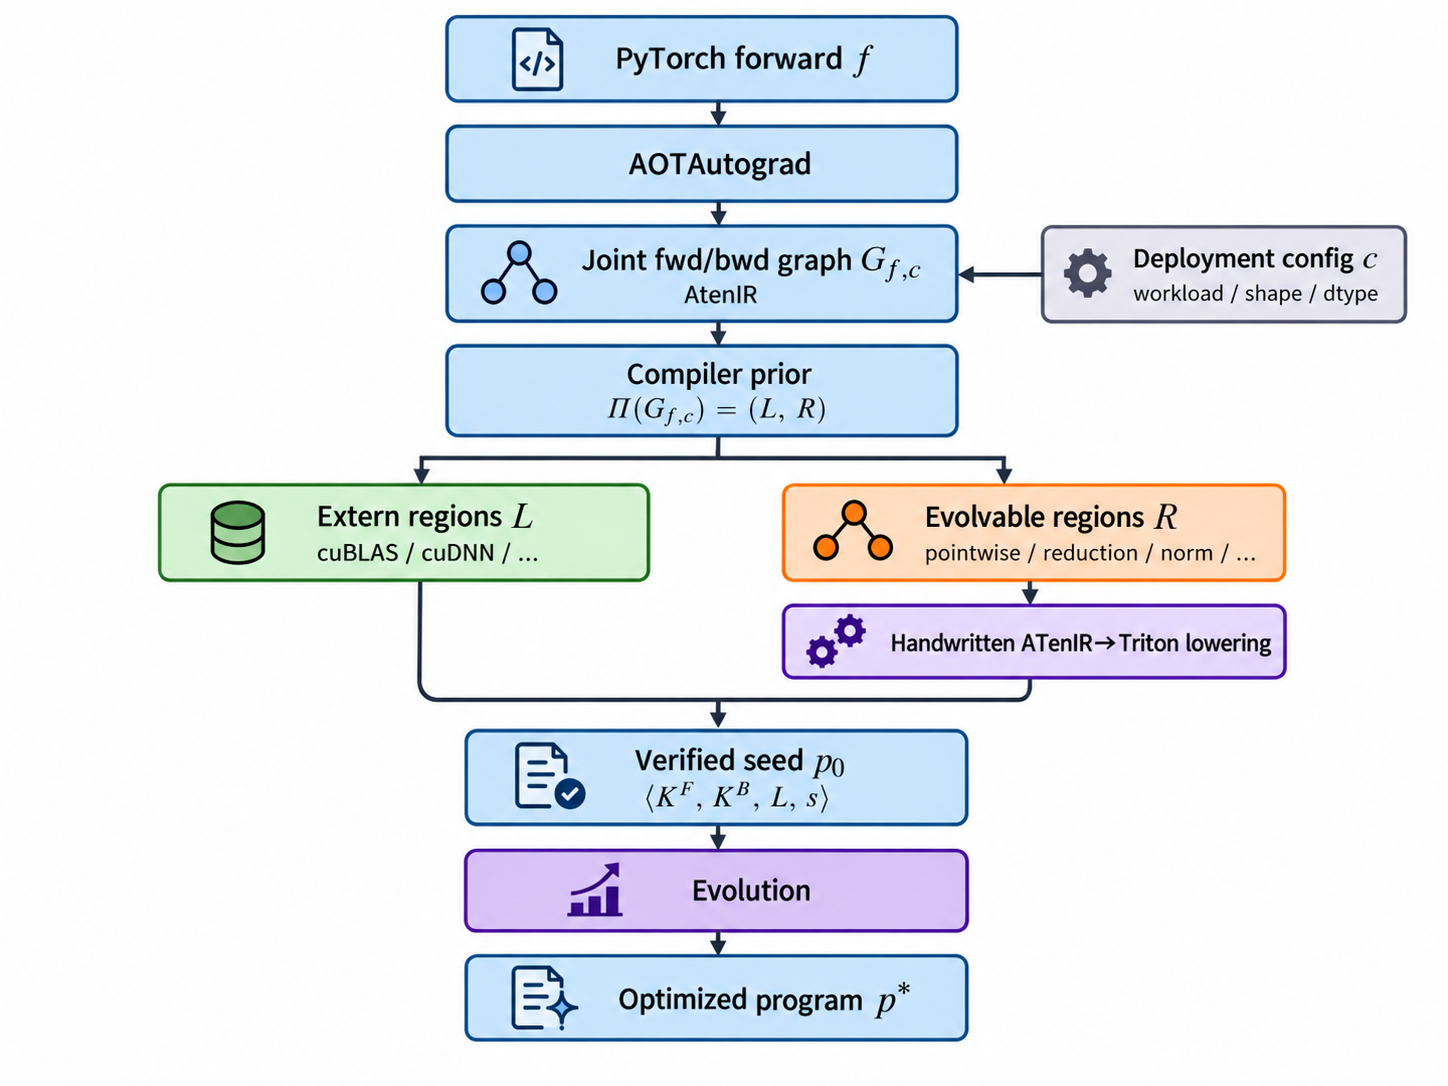
\includegraphics[width=\linewidth]{figures/evograd_pipeline.png}
    % Framework overview. The original seed-synthesis figure is retained alongside
% this editable diagram; the third stage makes deployment assessment explicit.
\begingroup
\small
\setlength{\fboxsep}{5pt}
\begin{tabular}{@{}c@{}}
PyTorch forward $f$ + workload configuration $c$ \\
$\downarrow$ \\
\fbox{\parbox{0.91\linewidth}{\centering
    \textbf{1. Seed synthesizer}\\[2pt]
    AOTAutograd $\rightarrow$ AtenIR $\rightarrow$ partition $(L,R)$\\
    Preserve library calls $L$; lower $R$ to Triton primitives
}} \\
$\downarrow\; p_0=\langle K_0^F,K_0^B,L,s_0\rangle$ \\
\fbox{\parbox{0.91\linewidth}{\centering
    \textbf{2. Agentic evolver}\\[2pt]
    Jointly refine forward, backward, and saved state\\
    $\circlearrowleft$ Local correctness checks and latency--memory score
}} \\
$\downarrow$ \\
\fbox{\parbox{0.91\linewidth}{\centering
    \textbf{3. Verifier + evaluator}\\[2pt]
    Check pair, integration, and training behavior\\
    Measure operator and training latency and memory\\
    Select qualifying replacements; reverify their combination
}} \\
$\downarrow$ \\
Accepted deployments with training measurements
\end{tabular}
\endgroup

    \caption{\method optimizes target AD kernels through compiler-guided synthesis and evolution, returning selected kernel implementations and bindings. The supplied model and workload support model-level verification and evaluation. Local checks and scores guide search; training measurements select qualifying replacements, whose combined deployment is verified again. External-library regions $L$ remain preserved.}
    \minjia{Please redraw the system overview figure to reflect our new framing. Instead dof showing ADopt as a standalone pipeline of seed synthesis, evolution, and verification/evaluation, we should explicitly show how ADopt integrates with PyTorch's compiler and runtime. The figure should show how ADopt starts from target operators in a PyTorch training workload, uses compiler-derived semantics to construct editable AD seeds, jointly optimizes forward/backward implementations and saved state, and integrates the generated kernels back into PyTorch for verification, evaluation, and deployment. Please also distinguish the lightweight feedback loop during agentic search from the more comprehensive deployment-time assessment, and make it clear where ADopt-Bench fits into this workflow. The key message is that ADopt develops kernels within the training framework in which they will be deployed.}
    \label{fig:evograd_pipeline}
\end{figure}

% \noindent\textbf{Training-implementation contract.}
% \label{sec:kernel-task}
% The specified primitive or composite operators define the kernel-optimization targets. Each kernel task is defined by its reference computation and configuration. The supplied model and prepared workload provide the context for verifying candidates and measuring their training impact; tasks with the same computation and configuration may be assessed in different training contexts. Section~\ref{sec:target_preparation} describes the prepared workloads and target operators.

% \noindent\textbf{Candidate implementation.}
% Each kernel task produces a candidate implementation $p$ comprising GPU kernels and forward and backward host code, $F_p$ and $B_p$, that launch them. \Appref{app:task_format} illustrates the task and deployment interfaces. Under configuration $c$, they satisfy
% \begin{equation}
%     (y,s_p)=F_p(x,\theta), \qquad
%     (\nabla_x,\nabla_\theta)=B_p(\nabla_y,s_p).
%     \label{eq:autograd_contract}
% \end{equation}
% Here, $s_p$ contains the state retained by $F_p$ for use in $B_p$, with its tensors determining the explicitly saved memory. The backward implementation returns the required vector--Jacobian products $\nabla_x=(\partial f/\partial x)^{\top}\nabla_y$ and $\nabla_\theta=(\partial f/\partial\theta)^{\top}\nabla_y$. Candidates may optimize forward and backward algorithms, fusion boundaries, which intermediates to retain or recompute, and permitted vendor-library calls. The pair is deployed through a \texttt{torch.autograd.Function}, allowing PyTorch autograd to invoke $B_p$ when the candidate runs as an operator or within its source model.

% \noindent\textbf{Selected output.}
% The returned set of implementations is
% \begin{equation}
%     \mathcal K_{\mathrm{selected}}
%     =\{(p_i,c_i,\sigma_i)\mid i\in I_{\mathrm{selected}}\},
%     \label{eq:selected_kernels}
% \end{equation}
% where $p_i$ contains a forward--backward implementation and its saved-state contract, $c_i$ is its supported configuration, and $\sigma_i$ binds it to the declared model sites. The verifier and evaluator select these implementations using their deployment evidence. Candidates are installed in the supplied model for verification and evaluation; the system returns optimized kernels and their deployment bindings. Targets without qualifying replacements retain their reference implementations, and an empty selected set indicates that no optimized kernel deployment qualified.

% For example, given a SwiGLU MLP kernel target, Qwen3-0.6B, and a prepared WikiText-2 workload, \method synthesizes and evolves the MLP implementation, verifies and evaluates it at the declared model sites, and returns a qualifying kernel implementation with its bindings.

% For a task $(f,c)$, \method searches the permitted program space $\mathcal{P}_{f,c}$. Reimplementing computations already served by mature vendor libraries adds unnecessary search effort, but directly evolving compiler-generated Triton code inherits the compiler's kernel boundaries, lowering, and scheduling decisions. \method instead preserves compiler-selected library calls while reconstructing the remaining computation from ATen semantics.





% \subsection{Compiler-Guided Seed Synthesizer}
\subsection{Compiler-Guided Seed Synthesis}
\label{sec:seed_synthesis}

% For each selected operator/configuration, the seed synthesizer constructs a structured starting program from training semantics, exposing joint forward--backward implementation choices without discarding compiler-selected library code.

The goal of seed synthesis is to construct a starting program that captures the semantics of a training operator while facilitating agentic optimization of its implementation. A natural approach is to provide the agent with the original PyTorch implementation and let it generate optimized forward and backward kernels. However, the backward computation and its dependencies on forward intermediates are implicit in the original implementation. The agent must derive these computations, determine their numerical requirements, and construct the saved-state interface before optimizing the kernels.

Another approach is to start from the GPU kernels generated by PyTorch's compiler. These kernels provide optimized implementations of the forward and backward computations. However, they represent one particular realization of the underlying AD computation, including specific kernel boundaries, computation strategies, and saved-state choices. For agentic optimization, we seek a program representation that preserves the underlying AD semantics while exposing these implementation choices as part of the search space.

\name constructs such a representation by leveraging the program semantics available in PyTorch's compiler. It synthesizes an executable forward--backward program, retains selected optimized library implementations, and exposes the remaining computations and saved-state interface to agentic optimization.

\noindent
\textbf{Forward--backward program representation.}
For each selected operator configuration, the kernel task provides a reference PyTorch forward computation, $y=f(x,\theta)$, where $x=(x_1,\ldots,x_n)$ is a tuple of input tensors, $\theta=(\theta_1,\ldots,\theta_m)$ a tuple of trainable parameter tensors, and $y=(y_1,\ldots,y_k)$ a tuple of forward outputs. The specification identifies the required outputs and the differentiable inputs and parameters for which gradients must be produced. Reference gradients are computed through PyTorch autograd with supplied upstream gradients $\nabla_y=(\nabla_{y_1},\ldots,\nabla_{y_k})$, one for each output. Each task fixes a configuration $c$ specifying tensor shapes, dtypes, memory layouts, and static operator parameters such as normalization epsilon. It is derived from the source-model training workload (Section~\ref{sec:workload_configs}). Static parameters remain fixed in $f$, while $x$, $\theta$, and $\nabla_y$ vary across instances. Reproducible generators support search-time timing, while recorded $(x,\theta,\nabla_y)$ instances from source-model execution supply verification and formal operator timing inputs in their original memory layouts.

\noindent\textbf{Candidate implementation.}
Each kernel task produces a candidate implementation $p$ comprising GPU kernels and forward and backward host code, $F_p$ and $B_p$, that launch them. \Appref{app:task_format} illustrates the task and deployment interfaces. Under configuration $c$, they satisfy
\begin{equation}
    (y,s_p)=F_p(x,\theta), \qquad
    (\nabla_x,\nabla_\theta)=B_p(\nabla_y,s_p).
    \label{eq:autograd_contract}
\end{equation}
Here, $s_p$ contains the state retained by $F_p$ for use in $B_p$, with its tensors determining the explicitly saved memory. The backward implementation returns the required vector--Jacobian products $\nabla_x=(\partial f/\partial x)^{\top}\nabla_y$ and $\nabla_\theta=(\partial f/\partial\theta)^{\top}\nabla_y$. Candidates may optimize forward and backward algorithms, fusion boundaries, which intermediates to retain or recompute, and permitted vendor-library calls. The pair is deployed through a \texttt{torch.autograd.Function}, allowing PyTorch autograd to invoke $B_p$ when the candidate runs as an operator or within its source model.

% \noindent\textbf{Autograd semantic extraction.}
\noindent\textbf{Extracting AD semantics.}
AOTAutograd derives the forward and backward computation of $f$ under configuration $c$. We represent it in AtenIR, a graph capturing ATen operators (e.g., \texttt{aten.add}, \texttt{aten.sum}, and \texttt{aten.mm}) and their data dependencies, without committing to kernel boundaries or schedules. Applying PyTorch's \texttt{min\_cut\_rematerialization\_partition} to the joint graph initializes the saved-state interface.

\noindent\textbf{Compiler-aware partitioning.}
For a task $(f,c)$, \method searches the permitted program space $\mathcal{P}_{f,c}$. Reimplementing computations already served by mature vendor libraries adds unnecessary search effort, but directly evolving compiler-generated Triton code inherits the compiler's kernel boundaries, lowering, and scheduling decisions. \method instead preserves compiler-selected library calls while reconstructing the remaining computation from ATen semantics.
We inspect TorchInductor's lowering decisions to partition the forward--backward computation as
\begin{equation}
    \Pi(G_{f,c}) = (L,R),
    \label{eq:partition}
\end{equation}
retaining its external-library assignments for operations such as dense GEMMs and convolutions backed by cuBLAS and cuDNN.

\noindent\textbf{Semantic resynthesis.}
For $R$, handwritten lowering rules map supported AtenIR operations to pre-implemented Triton primitives and generate host code that invokes them according to data dependencies. The primitives and host code implement broadcasting, dtype conversion, and reduction semantics. This deterministically constructs the seed without LLM-based synthesis or cross-operator fusion; its primitive boundaries remain open to rewriting during evolution. Combining the synthesized computation with $L$ yields
\begin{equation}
    p_0 =
    \left\langle
        K_0^F,\,
        K_0^B,\,
        L,\,
        s_0
    \right\rangle,
    \label{eq:seed_program}
\end{equation}
where $K_0^F$ and $K_0^B$ denote the synthesized forward and backward kernels with their host code, $L$ contains the preserved library calls, and $s_0$ is the state passed from forward to backward. \Appref{app:seed_example} illustrates these components with a masked linear map.

\noindent\textbf{Constructing the search space.} 
% Let $L$ denote the preserved external-library regions, $R$ the remaining ATen computation, and $\mathcal{P}_{f,c}^{L}\subseteq\mathcal{P}_{f,c}$ the candidate space that preserves $L$ while allowing different implementations and saved-state choices for $R$. 
Let $L$ denote the computations served by the preserved external library calls and $R$ denote the remaining ATen computations. For a target computation $f$ and configuration $c$, the synthesized seed defines an implementation space $\mathcal{P}_{f,c}^{L}$ in which the agent can explore alternative kernel implementations, fusion strategies, and saved-state representations for $R$ while retaining the optimized library calls in $L$ and preserving the external AD contract.


\subsection{Agentic Evolver}
\label{sec:evolution}

An AD kernel replaces both the forward and backward implementations of a differentiable operator in the training framework. Its optimization objective must therefore account for the combined execution latency of both passes and the memory required to retain intermediate state between them. Given a compiler-guided seed, \method jointly optimizes the forward and backward implementations and their saved-state interface while preserving the operator's external AD semantics.

Given the synthesized seed and its associated implementation space $\mathcal{P}_{f,c}^{L}$, \method searches for an implementation that improves forward-backward execution efficiency while reducing saved-state memory. The objective is
\begin{equation}
    p^\star
    \in
    \operatorname*{arg\,max}_{p\in\mathcal{P}_{f,c}^{L}}
    \operatorname{Score}(p;c)
    \quad \text{subject to} \quad
    \mathcal{V}(p,f,c)=1,
    \label{eq:objective}
\end{equation}
where $\operatorname{Score}(p;c)=Q(p;c)$ is the Tier~1 search score in Equation~\ref{eq:tier1_search_score}, and $\mathcal{V}$ is the verification predicate in Equation~\ref{eq:validity}. This objective guides local search; the evaluator subsequently uses training measurements to select qualifying replacements for combined deployment.

% The synthesized pair provides a checked starting implementation; evolution explores alternative kernels, orchestration, and saved-state representations. 
Unlike conventional kernel optimization workflows that operate on individual GPU kernels, \method presents the complete forward--backward program to the agent as the unit of optimization. The program includes the GPU kernels, host code that orchestrates their execution, external library calls, and the state passed between the forward and backward computations.
Starting from the verified seed $p_0$, \method uses OpenEvolve to optimize Equation~\ref{eq:objective}. Search can modify the synthesized Triton kernels, host code, and saved-state policy while preserving $L$ and the public autograd interface. Candidates must pass search-time correctness checks before timing and scoring; failures are rejected. Selected final candidates undergo the applicable verification and evaluation protocols in Sections~\ref{sec:verification_protocol} and~\ref{sec:evaluation_protocol}.

\minjia{I think this is one of the most important parts of the paper, but currently I don't get a good sense of how the agent actually optimizes an AD kernel. What does the agent see? What can it change? What feedback does it receive, and how does that feedback help it improve the implementation? It would be also interesting to walk through a real example where the agent makes coordinated changes to the forward and backward computations or redesigns the saved state. This would help readers understand what joint optimization actually buys us. Finally, clarify which parts of the workflow are specific to ADopt and which are provided by the underlying evolver. Ideally, OpenEvolve is just one instance of the agentic optimization framework, not an essential part of our design.}

% \subsection{Deployment Verifier}
\subsection{Progressive Correctness Verification}
\label{sec:verification_protocol}

Verifying an agent-generated AD kernel requires more than checking its forward and backward pass in isolation. The implementation must also behave correctly when invoked by PyTorch's autograd engine, interact with other operators in the model, preserve numerical accuracy across training updates. However, verifying every candidate through whole model training would be expensive. \system there uses progressive verification, with three levels of increasing execution scope and verification cost:
% \method uses three verification gates: 
% local pair verification, single-step framework integration verification, 
local AD kernel verification, framework integration verification, and multi-step training verification,
\minjia{I added the rationale for this progressive verification protocol and also updated the names of the three verification steps. Please update the following notations, perhaps local, int, train, and make sure the notations are consistent.}
% and multi-step training verification, 
with binary outcomes $\mathcal{V}_{\mathrm{pair}}$, $\mathcal{V}_{\mathrm{int}}$, and $\mathcal{V}_{\mathrm{train}}$, respectively.
The applicable gate set $\mathcal{G}_{f,c}$ depends on the target granularity and the supplied model/workload. For candidates satisfying the task's static rules, acceptance requires
\begin{equation}
    \mathcal{V}(p,f,c)
    =
    \bigwedge_{g\in\mathcal{G}_{f,c}}
    \mathcal{V}_g(p,f,c)
    =1.
    \label{eq:validity}
\end{equation}
Pair verification asks whether the forward--backward pair computes the declared function. Integration verification asks whether the candidate remains accurate when deployed through PyTorch autograd, as an operator and within the source model. Training verification asks whether its numerical differences compound over successive optimizer updates. A gate passes only if the candidate executes completely and meets every structural and numerical criterion.

Floating-point arithmetic admits no single correct result: two correct implementations of the same computation differ by rounding, and a model can amplify such differences. Every numerical criterion therefore takes the same form: the candidate's error must not exceed the larger of a fixed floor and a multiple of the error of trusted implementations of the same computation, measured on the same inputs. The trusted implementations are the source model's native execution and its \texttt{torch.compile} compilation; thresholds depend only on them, never on the candidate. 

During search, the evolver applies Gate~1 to a subset of the recorded calls to admit candidates for scoring; deployment verification then runs the full gates. A primitive candidate must pass pair verification and operator-scope integration verification. A composite candidate must additionally pass model-scope integration and training verification where available, with the candidate installed alone at its site in the supplied model. Selected composite candidates deployed together are verified again by model-scope integration and training verification. Only deployments passing all required gates contribute to the main performance results. All verification uses PyTorch's deterministic settings and runs outside timed regions. Model-specific gate availability, configurations, and detailed procedures are provided in \appref{app:verification_details}.

\noindent\textbf{Gate 1: Local pair verification ($\mathcal{V}_{\mathrm{pair}}$).}
Gate~1 asks whether the pair computes the declared function. It directly invokes the candidate's forward and backward implementations, $F_p$ and $B_p$, with $B_p$ consuming the candidate's own saved state $s_p$, and compares every declared forward output and the gradient of every differentiable input and parameter with the reference computation $f$ under PyTorch autograd; the internal decomposition and saved state need not match the reference.

The gate replays calls recorded from source-model training on real-world datasets, preserving their inputs, parameters, upstream gradients, and memory layouts. For each such tensor $z$, the reference $z^{\mathrm{ref}}$ is $f$ evaluated in float32, so that a candidate is not penalized for being more accurate than the model's reduced-precision arithmetic, and $z^{\mathrm{native}}$ is $f$ at the model's own dtypes. With $d(a,b)=\|a-b\|_\infty/\|b\|_\infty$, the candidate must satisfy on every call
\begin{equation}
d(z^{\mathrm{cand}},z^{\mathrm{ref}})
\leq \max\Bigl\{\beta_1,\;\gamma_1\max_{\mathrm{calls}}d(z^{\mathrm{native}},z^{\mathrm{ref}})\Bigr\},
\label{eq:local_numerical_contract}
\end{equation}
where $\beta_1$ is a floor fixed per dtype and $\gamma_1=2$ is a safety margin, as in the kernel tests of FlashAttention~\cite{dao2022flashattention}. The floor decides for most results; the native term takes over where large terms nearly cancel, as in attention gradients, and native execution itself exceeds the floor. Acceptance also requires the declared structure, shape, and dtype, finite results, and no input mutation unless permitted by the task.


\noindent\textbf{Gate 2: Framework integration verification ($\mathcal{V}_{\mathrm{int}}$).}
Gate~2 checks the candidate through its deployment path in PyTorch autograd. At \emph{operator scope}, it replays recorded calls and compares the same outputs and gradients as Gate~1, isolating local error. At \emph{model scope}, it compares model outputs, loss, and every trainable parameter's gradient, capturing error propagation and interactions among replacements. Each replaced site then receives inputs computed by the modified model, allowing local errors to affect downstream computations and exposing deployment faults such as skipped sites. Candidate and native eager executions perform one forward and backward pass under matched inputs, parameters, random states, and numerical settings, without an optimizer update.

A sample $x$ is one recorded call at operator scope and one workload batch at model scope. For each required floating-point result tensor $z$, we measure
\begin{equation}
\begin{aligned}
E_2(z;x)
&=\frac{\|z_x^{\mathrm{cand}}-z_x^{\mathrm{ref}}\|_2}{\max(\|z_x^{\mathrm{ref}}\|_2,\epsilon)},\\
E_{\max}(z;x)
&=\frac{\|z_x^{\mathrm{cand}}-z_x^{\mathrm{ref}}\|_\infty}{\max(\operatorname{RMS}(z_x^{\mathrm{ref}}),\epsilon)},
\end{aligned}
\label{eq:integration_errors}
\end{equation}
where $\operatorname{RMS}(z)=\sqrt{n_z^{-1}\sum_i z_i^2}$ over the $n_z$ elements of $z$, and $\epsilon=10^{-30}$ guards against division by zero. $E_2$ measures error across the tensor, including small discrepancies spread across many elements; $E_{\max}$ catches errors confined to a few elements that contribute little to $E_2$. Its normalization uses the tensor's typical magnitude rather than individual near-zero elements.

For each result tensor $z$ and metric $m\in\{2,\max\}$, let $D_m(z;x)$ be the larger of the native-repeat and compile--native discrepancies on calibration sample $x$. The threshold is
\begin{equation}
T_{z,m}=\gamma\max\left\{\max_{x\in\mathcal{C}}D_m(z;x),\,f_{z,m}\right\},
\label{eq:integration_calibration}
\end{equation}
where $\mathcal{C}$ is the calibration set, $f_{z,m}>0$ is a floor, and $\gamma>1$ is a fixed scope-specific safety margin. Operator scope uses separate calibration and acceptance calls; model scope verifies fresh executions of the calibrated inputs. Every required result on every verification sample must satisfy
\begin{equation}
E_2(z;x)\leq T_{z,2}
\quad\land\quad
E_{\max}(z;x)\leq T_{z,\max},
\label{eq:integration_acceptance}
\end{equation}
together with Gate~1's structure, shape, dtype, finiteness, and input-mutation checks. Model scope additionally requires unchanged parameters and the declared call count at every replaced site.

\noindent\textbf{Gate 3: Multi-step training verification ($\mathcal{V}_{\mathrm{train}}$).}
Gate~3 checks whether numerical differences compound through successive gradient computations and optimizer updates on real-world datasets. Each update changes the weights and optimizer state used by later steps, allowing differences that are small in a single forward--backward pass to grow along the training trajectory. Where available, it follows Gates~1 and~2 for individual composite candidates and their combined deployments. Candidate and native eager runs start from identical model and optimizer states and use the same training batches, random states, numerical settings, and optimizer schedule. Neither run is reset to the other's state.

Let $\ell_t^p$ be the training loss differentiated at update $t$ of run $p$, and let $d_t^p=\ell_t^p-\ell_t^{\mathrm{native}}$. Over all $N$ updates, we measure
\begin{equation}
R_p=\sqrt{\frac{1}{N}\sum_{t=1}^{N}(d_t^p)^2},
\qquad
M_p=\max_{1\leq t\leq N}|d_t^p|.
\label{eq:training_errors}
\end{equation}
$R_p$ measures the root mean square loss difference, preventing cancellation across updates; $M_p$ bounds the largest single-step difference. Both use the full trajectory, without windows or excluded steps.

Acceptance requires
\begin{equation}
R_{\mathrm{cand}}\leq T_R
\quad\land\quad
M_{\mathrm{cand}}\leq T_M,
\label{eq:training_acceptance}
\end{equation}
where $T_R$ and $T_M$ are frozen from native-repeat and compiled-control trajectories with positive floors and a safety margin. The candidate must complete all $N$ updates with finite losses and execute every replaced site at each update.

% \subsection{Correctness Verification Protocol}
% \label{sec:verification_protocol}

% \bench verifies candidate correctness through three complementary gates introduced in Section~\ref{sec:benchmark-task}: local pair verification ($\mathcal{V}_{\mathrm{pair}}$), single-step framework integration verification ($\mathcal{V}_{\mathrm{int}}$), and multi-step training verification ($\mathcal{V}_{\mathrm{train}}$). These gates check the declared forward--backward computation, its integration into the framework, and its numerical behavior over continuous training updates. The verification gates compare the candidate with the reference computation of the source model and accept it only if its error stays within a threshold calibrated from trusted controls: repeated native executions, which measure run-to-run variation, and a \texttt{torch.compile} implementation of the same reference, which measures how far a correct alternative implementation departs from native. Thresholds are frozen before any candidate is evaluated.

% A Level~1 candidate must pass pair verification and operator-scope integration verification. A Level~2 candidate must additionally pass model-scope integration and training verification with the candidate installed alone at its site in the source model. Selected Level~2 candidates deployed together for Level~3 are verified again by the model-scope integration and training gates. Only deployments passing all required gates contribute to the main performance results. All verification uses PyTorch's deterministic settings and runs outside timed regions. Model-specific configurations and detailed procedures are provided in Appendix~\ref{app:verification_details}.

% \paragraph{Gate 1: Local pair verification ($\mathcal{V}_{\mathrm{pair}}$).}
% Gate~1 directly invokes the candidate's forward and backward implementations, $F_p$ and $B_p$, and compares every declared forward output and every required input and parameter gradient against the source-model reference $f$ under PyTorch autograd, element by element. The candidate's internal decomposition and saved state $s_p$ need not match the reference.

% Its inputs are recorded from training steps of the source model on real data: every invocation of the task, with its inputs, parameters, and upstream gradients in their original memory layouts. Thresholds are calibrated, and candidates are verified on invocations from different training batches (Appendix~\ref{app:recorded_calls}). For each result tensor $z$, every element must satisfy
% \begin{equation}
% \left|z_i^{\mathrm{cand}}-z_i^{\mathrm{ref}}\right|
% \leq \max\!\left(a_z+r_z\left|z_i^{\mathrm{ref}}\right|,\; \gamma_{\mathrm{op}}\Delta_z\right),
% \label{eq:local_numerical_contract}
% \end{equation}
% where $z$ is a required output or gradient, $a_z$ and $r_z$ are the default tolerances of \texttt{torch.testing.assert\_close} for the dtype of $z$ (Appendix~\ref{app:gate1_tolerances}), $\Delta_z$ is the largest elementwise difference between the \texttt{torch.compile} control and native execution on $z$ over the calibration batches, and $\gamma_{\mathrm{op}}>1$ is a safety margin.

% The first term is the standard PyTorch tolerance; it alone would reject correct implementations where two large terms nearly cancel, as in rotary embeddings, the rounding error grows with the size of the two terms, while the allowed error shrinks with the near-zero result, and \texttt{torch.compile} itself violates it there. The second term therefore admits any error up to $\gamma_{\mathrm{op}}$ times what \texttt{torch.compile} shows on the same result, so the bound is never stricter than a trusted compiler's own rounding, and it relaxes only the results on which such deviations are observed. The gate passes only if every element satisfies this bound, every result has the declared structure, shape, and dtype and is finite, and no input is modified unless the task permits it.


% \paragraph{Gate 2: Framework integration verification ($\mathcal{V}_{\mathrm{int}}$).}
% Gate~2 checks candidates through their actual PyTorch-autograd deployment paths at operator scope (L1 and L2) and whole-model scope (L3). The reference is the corresponding computation extracted from the pinned source-model implementation, or the unmodified model. Candidate and native eager executions perform one forward and backward pass under matched inputs, parameters, random conditions, and numerical settings, without an optimizer update.

% \paragraph{Gate 2: Framework integration verification ($\mathcal{V}_{\mathrm{int}}$).}
% Gate~2 checks the candidate as it is deployed in training. It runs the candidate through its deployment path in PyTorch autograd and compares whole tensors against thresholds calibrated from trusted controls, which detects faults in the deployment code and small errors spread across a tensor that an elementwise tolerance admits. It does so at two scopes. \textbf{Operator scope} gives every call the inputs recorded from native training, isolating the candidate's own error. \textbf{Model scope} runs candidates inside the source model, so each receives inputs computed by the modified model, its error propagates to the loss and every parameter gradient, errors of several candidates can compound, and deployment faults such as a skipped site become visible. Every candidate is checked at operator scope. Each Level-2 candidate is also checked at model scope alone at its site, and the Level-2 candidates that pass verification and speed up training are checked together as the Level-3 candidate. Level-1 candidates are checked at operator scope only, since a single primitive is too small a part of the model for whole-model results to judge it.

% At both scopes, the candidate is compared with native eager execution of the source model's own code over one forward and backward pass, under matched inputs, parameters, random states, and numerical settings, without an optimizer update. Operator scope uses the recorded calls of Gate~1 and compares every declared output and every required input and parameter gradient. Model scope runs one training step on real training batches, compares the model output, the loss, and every trainable parameter's gradient, and checks that each replaced site is called the declared number of times and that inputs and parameters remain unchanged.

% A sample $x$ is one recorded call at operator scope and one training batch at model scope. For each required floating-point result tensor $z$ on sample $x$, we measure
% \begin{equation}
% \begin{aligned}
% E_2(z;x)
% &=\frac{\|z_x^{\mathrm{cand}}-z_x^{\mathrm{ref}}\|_2}{\max(\|z_x^{\mathrm{ref}}\|_2,\epsilon)},\\
% E_{\max}(z;x)
% &=\frac{\|z_x^{\mathrm{cand}}-z_x^{\mathrm{ref}}\|_\infty}{\max(\operatorname{RMS}(z_x^{\mathrm{ref}}),\epsilon)},
% \end{aligned}
% \label{eq:integration_errors}
% \end{equation}
% where $\operatorname{RMS}(z)=\sqrt{n_z^{-1}\sum_i z_i^2}$ over the $n_z$ elements of $z$, and $\epsilon=10^{-30}$ only guards against division by zero. $E_2$ is the relative error of the whole tensor and accumulates small errors spread across all elements; $E_{\max}$ bounds the largest single-element error relative to the tensor's typical magnitude, which catches errors confined to a few elements that $E_2$ averages out, without inflating errors at near-zero elements.

% As in Gate~1, thresholds are calibrated from two controls before any candidate is verified: a native repeat, which measures run-to-run variation, and the \texttt{torch.compile} control at the candidate's sites, which measures the difference between two correct implementations. Both run deterministically with matched random states (Appendix~\ref{app:determinism}). For each result tensor $z$ and metric $m\in\{2,\max\}$, the control discrepancy on sample $x$ is
% \begin{equation}
% \begin{aligned}
% D_m(z;x)=\max\bigl\{&
% E_m\!\left(z_x^{\mathrm{native},2},z_x^{\mathrm{native},1}\right),\\
% & E_m\!\left(z_x^{\mathrm{compile}},z_x^{\mathrm{native},1}\right)
% \bigr\}.
% \end{aligned}
% \label{eq:integration_control_error}
% \end{equation}

% The threshold for $z$ and $m$ takes the largest control discrepancy over a set of calibration samples $\mathcal{C}$:
% \begin{equation}
% T_{z,m}=\gamma\max\left\{\max_{x\in\mathcal{C}}D_m(z;x),\,f_{z,m}\right\}.
% \label{eq:integration_calibration}
% \end{equation}
% At operator scope, $\mathcal{C}$ holds the calls recorded from the calibration batches, including calls of the same configuration from different layers; candidates are judged on calls from the other batches, and $\gamma=\gamma_{\mathrm{op}}$. At model scope, $\mathcal{C}$ holds four training batches, candidates are judged on fresh executions of the same batches, and $\gamma=\gamma_{\mathrm{model}}$. The floor $f_{z,m}$ keeps the threshold positive when both controls reproduce native execution exactly. Floors and safety margins are given in Appendix~\ref{app:gate2_thresholds}. Gate~3 follows the same calibration principle with training-trajectory metrics.

% Acceptance requires every required result on every verification sample to satisfy
% \begin{equation}
% E_2(z;x)\leq T_{z,2}
% \quad\land\quad
% E_{\max}(z;x)\leq T_{z,\max},
% \label{eq:integration_acceptance}
% \end{equation}
% together with the structure, shape, dtype, finiteness, and input-mutation checks of Gate~1 and, at model scope, the site-call and parameter checks above.

% % \ahan{You sort of lost me here. I do not understand what calibration means. It also sort of comes out of nowhere since we are talking about each tier's correctness gate.}

% % \wangjia{Calibration is the procedure for setting thresholds from trusted native and compiled executions before evaluating a candidate; $T$ denotes the resulting threshold. It is part of the correctness checks, not an additional gate.}

% \paragraph{Gate 3: Multi-step training verification ($\mathcal{V}_{\mathrm{train}}$).}
% Gate~3 checks how numerical differences propagate through successive gradient computations and optimizer updates on real training data: each update changes the weights and optimizer state that later steps see, so small per-step differences can compound over training. It applies where model-scope Gate~2 does, to each Level-2 candidate alone at its site and to the Level-3 candidate, after they pass Gates~1 and~2. Candidate and native eager runs start from identical model and optimizer states and use the same training batches, random states, numerical settings, and optimizer schedule (Appendix~\ref{app:gate3_settings}). Neither run is reset to the other's state, so differences accumulate as they would in training.


% Let $\ell_t^p$ be the training loss that update $t$ of run $p$ differentiates, and let $d_t^p=\ell_t^p-\ell_t^{\mathrm{native}}$. Over the $N$ updates of a run, we measure
% \begin{equation}
% R_p=\sqrt{\frac{1}{N}\sum_{t=1}^{N}(d_t^p)^2},
% \qquad
% M_p=\max_{1\leq t\leq N}|d_t^p|.
% \label{eq:training_errors}
% \end{equation}
% $R_p$ is the root mean square of the loss difference, so differences of opposite sign do not cancel; $M_p$ bounds the largest single-step difference. Both use every update of the run, without windows or excluded steps.


% Following Gate~2's calibration principle (Equations~\ref{eq:integration_control_error}--\ref{eq:integration_calibration}), thresholds are calibrated before any candidate is verified, from a native repeat and the \texttt{torch.compile} control at the candidate's sites, each trained under the same conditions:
% \begin{equation}
% \begin{aligned}
% T_R&=\gamma_{\mathrm{train}}\max\{R_{\mathrm{repeat}},R_{\mathrm{compile}},f_R\},\\
% T_M&=\gamma_{\mathrm{train}}\max\{M_{\mathrm{repeat}},M_{\mathrm{compile}},f_M\},
% \end{aligned}
% \label{eq:training_calibration}
% \end{equation}

% where $f_R$ and $f_M$ are floors and $\gamma_{\mathrm{train}}>1$ is a safety margin (Appendix~\ref{app:gate3_settings}).

% Acceptance requires
% \begin{equation}
% R_{\mathrm{cand}}\leq T_R
% \quad\land\quad
% M_{\mathrm{cand}}\leq T_M,
% \label{eq:training_acceptance}
% \end{equation}
% and the candidate run must complete all $N$ updates with a finite loss at every step.



% \ahan{How do we decide the window length? This seems to be key to this correctness gate. Also this particular design choice deviates from L1 and L2 checks. L1 and L2 work on per-element. However, for some reason this level seems to be much more lax with the correctness check. I understand the difficulty: training is noisy at the start and perhaps per-step loss is hard to inform correctness. But if this is the case motivate this check by stating this before introducing windowing.}
% \wangjia{We revised the gate after exploring per-step thresholds and windowed comparisons. Per-step control-derived thresholds were overly sensitive to when control discrepancies occurred: a small discrepancy at one step could create a tight local budget despite larger deviations elsewhere. Windowed mean-loss comparisons introduce an additional length parameter and can dilute spikes or cancel signed differences. We therefore use full-trajectory RMS together with maximum absolute error, avoiding a window-length choice while measuring both overall and peak deviations. The motivation is accumulated numerical divergence between independently updated states, rather than uncontrolled training noise. This complements, rather than replaces, the output and gradient checks in earlier gates. It sacrifices step-specific sensitivity, so it is a finite-horizon training-behavior check, not proof of identical training dynamics. Also, Gate~2 uses tensor-level error metrics rather than per-element acceptance.}

% \ahan{How are the inputs generated for this stage? Is it still random, or is it now on legitimate data?}
% \wangjia{We construct training workloads from real datasets rather than synthetic inputs. For Qwen3-0.6B, we use the training split of WikiText-2. I will mention this in the main table for this section.}


% \subsection{Performance Evaluation Protocol}
% \label{sec:evaluation_protocol}

% A faster kernel need not yield faster training. \bench uses Tier~1 for search and diagnostics and Tiers~2--3 for deployment performance. Only candidates passing all applicable verification gates contribute to the main results. Timing and statistical details appear in Appendix~\ref{app:evaluation_details}.

% For candidate provider $p$, baseline $b$, configuration $c$, and tier $t\in\{2,3\}$, speedup is
% \begin{equation}
% S^t_{p/b}(c)=\frac{T^t_b(c)}{T^t_p(c)},
% \label{eq:evaluation_speedup}
% \end{equation}
% where $T^t$ denotes the tier's execution time. Baselines are eager PyTorch and \texttt{torch.compile} where available.

% \noindent\textbf{Tier 1: isolated forward--backward pair.}
% Tier~1 asks whether a candidate improves execution efficiency during search. We invoke $F_p$ and $B_p$ directly without autograd. Backward timing excludes preparation of saved state $s_p$; pair timing executes $F_p$ then $B_p$ within one timed region. Their reference-to-candidate timing ratios and a saved-memory penalty guide search only.

% \noindent\textbf{Tier 2: deployed operator.}
% Tier~2 asks whether the candidate accelerates operator execution through PyTorch autograd. Providers replay the corpus of calls recorded from native training for each configuration, matching inputs, parameters, upstream gradients, memory layouts, and autograd execution boundaries. $T^2_p(c)$ sums per-call median forward--backward latencies; speedups include 95\% bootstrap intervals.

% \noindent\textbf{Tier 3: whole-model training.}
% Tier~3 asks whether Level~2 candidates accelerate whole-model training. We time complete steps, including forward/loss, backward, optimizer update, and gradient reset. Within each system and model, accepted candidates whose individual eager-relative 95\% speedup intervals have lower bounds above one are combined, reverified under applicable model-scope gates, and retimed against both baselines.

% \noindent\textbf{Memory and Coverage.}
% Tier~1 reports logical saved-state bytes; Tier~3 reports peak allocated GPU memory relative to eager. Level~1/2 coverage is the fraction of all observed configurations with executable, accepted candidates, including unsubmitted and unselected configurations in the denominator.

% \subsection{Multi-Level Evaluator and Deployment Selection}
\subsection{Training-Integrated Performance Evaluation}
\label{sec:evaluation_protocol}
% \minjia{I think Sections 3.4 and 3.5 overlap quite a bit. Both essentially introduce three levels of execution, but one focuses on correctness and the other on performance. Can we unify them into a single section on training-integrated kernel assessment/evaluation? We can explain the rationale and execution mechanism at each level once, and then describe what we verify and measure. Kernel selection and deployment can be a separate subsection. This would reduce redundancy and present a more coherent design, especially since the assessment infrastructure is also used by ADopt-Bench. Thoughts?}

A faster kernel does not necessarily produce a faster training step. Framework overhead, surrounding computation, and operator frequency determine how much an isolated speedup contributes to training performance. The evaluator measures performance at three scopes: the isolated forward--backward pair, operator execution through PyTorch autograd, and whole-model training. Tier~1 supports search and diagnostics, while Tiers~2 and~3 provide the main deployment performance results. Training measurements select individually beneficial replacements for combined deployment, which is verified and measured again. We use the same protocols to assess \method and the other kernel workflows in the prepared model workloads. Detailed timing, memory, and aggregation procedures appear in \appref{app:evaluation_details}.

Formal comparisons use matched inputs and execution conditions. Verification runs outside timed regions; executable candidates that fail verification may retain diagnostic timings, but only deployments passing all applicable gates contribute to the main results. We report speedup as
\begin{equation}
    S^t_{p/b}(c) = \frac{T^t_b(c)}{T^t_p(c)},
    \label{eq:evaluation_speedup}
\end{equation}
where $p$ is the candidate provider, $b$ the baseline, $c$ the workload configuration, and $t$ the measurement tier. $T^t$ denotes the execution time defined at that tier. Values above one indicate faster execution. Baselines are eager PyTorch and \texttt{torch.compile} where applicable.

\paragraph{Tier 1: isolated forward--backward pair.}
Tier~1 asks whether a candidate improves execution efficiency during search. It directly invokes $F_p$ and $B_p$ without the PyTorch autograd engine. We measure backward alone, preparing the saved state $s_p$ outside the timed region, and the complete forward--backward pair within one timed region. Backward-only timing measures gradient computation from saved state, while pair timing captures tradeoffs that shift work between forward and backward or replace saved state with recomputation.

For candidates passing the search correctness checks, the default search score is
\begin{equation}
    Q(p;c)
    =
    \frac{(1-\alpha)\rho_{\mathrm{bwd}}(p;c)
          +\alpha\rho_{\mathrm{pair}}(p;c)}
         {1+\lambda R_{\mathrm{saved}}(p;c)},
    \label{eq:tier1_search_score}
\end{equation}
where $\rho_{\mathrm{bwd}}$ and $\rho_{\mathrm{pair}}$ are reference-to-candidate timing ratios for backward and the complete pair, and $R_{\mathrm{saved}}$ is defined below. The default weights are $\alpha=0.5$ and $\lambda=0.05$. These ratios guide search but are not reported as performance speedups because reference and candidate use different execution paths.

\paragraph{Tier 2: deployed operator.}
Tier~2 asks whether the candidate is faster than eager PyTorch and \texttt{torch.compile} through its deployment path in PyTorch autograd. All providers execute forward and backward through the autograd engine under matched execution boundaries, so comparisons include the framework costs of deploying the operator. We replay all recorded calls of each configuration from one native training step, with identical inputs, parameters, upstream gradients, and memory layouts across providers. The Tier~2 time $T^2_p(c)$ sums the per-call median forward--backward latencies, capturing variation across repeated calls and model layers. Speedup follows Equation~\ref{eq:evaluation_speedup}, with 95\% bootstrap intervals. Only candidates passing all applicable verification gates contribute to the main results.

\paragraph{Tier 3: whole-model training.}
Tier~3 asks whether operator-level improvements translate into faster whole-model training. For supported workloads, we install composite candidates at their declared model sites and time complete steps, including forward execution, loss computation, backward propagation, optimizer update, and gradient reset. We first measure each candidate alone against eager. For each system and model, we then combine accepted candidates whose single-site speedup has a 95\% interval with its lower bound above one. The combination is verified again by model-scope integration and training verification, and measured against eager and whole-model \texttt{torch.compile} where available. Individual and combined measurements distinguish local contributions from interactions among replacements.

\paragraph{Selected implementations.}
The evaluator returns the selected kernel implementations with their supported configurations and model-site bindings. Their joint deployment must pass the applicable model-scope gates before it is reported as a qualifying combination. A failed or incomplete combination remains reported as such; individual acceptance does not establish combined correctness. Sites without selected replacements use the native computation.

\paragraph{Memory.}
We record logical saved-state memory at Tier~1 and peak allocated GPU memory at Tier~3 to characterize the tradeoff between execution time and memory use. For operator pairs, normalized saved-state memory is
\begin{equation}
    R_{\mathrm{saved}}(p;c)
    =
    \frac{M_p^{\mathrm{saved}}(c)}
         {M_{\mathrm{input}}(c)},
    \label{eq:saved_memory_ratio}
\end{equation}
where $M_p^{\mathrm{saved}}$ counts tensor bytes explicitly retained in $s_p$, and $M_{\mathrm{input}}$ counts the task's declared memory inputs. Whole-model peak allocation is measured in a separate untimed step after optimizer-state initialization and reported relative to eager.

\paragraph{Coverage.}
Alongside performance, we report acceptance coverage: the fraction of observed configurations with executable candidates that pass all applicable verification gates. Failed and unsubmitted configurations remain in the denominator, so coverage reflects the scope of successful implementations rather than their speed alone.










% \paragraph{Tier 2: deployed operator.}
% Tier~2 asks whether the candidate is faster than eager PyTorch and \texttt{torch.compile} through its deployment path in PyTorch autograd. All providers execute forward and backward through the autograd engine under matched execution boundaries, so comparisons include the framework costs of deploying the operator. We replay all recorded calls of each configuration from one native training step, with identical inputs, parameters, upstream gradients, and memory layouts across providers. The Tier~2 time $T^2_p(c)$ sums the per-call median forward--backward latencies, capturing variation across repeated calls and model layers. Speedup follows Equation~\ref{eq:evaluation_speedup}, with 95\% bootstrap intervals. Only candidates passing all applicable verification gates contribute to the main results. Timing and statistical details appear in Appendix~\ref{app:tier2_timing}.

% % \paragraph{Tier 3: block and model.}
% % Tier~3 measures what practitioners ultimately care about: the training step. Candidates are installed at a workload's declared replacement sites, with native implementations everywhere else. An operator's effect on the step depends on how often it runs, its share of step time, and how it interacts with its neighbors, none of which the lower tiers can see. Measuring each site alone and in combination separates a site's own contribution from these interactions. Block scope is a middle ground: a single architectural block supplies local context without the cost and noise of a full model. Model scope times complete training steps, including loss, backward, and the optimizer update, on warm caches as in real training. Because a step can be limited by the host rather than the GPU, we also record how much of the step the host spends issuing work; when the host dominates, no kernel improvement can appear. Two controls keep the comparison honest. Activation checkpointing is held fixed across providers and recorded, since recomputation changes how often each kernel runs.

% \paragraph{Tier 3: block- and model-level training.}
% Tier~3 asks whether the operator-level improvement translates into faster training when the optimized operator is embedded in the computation that surrounds it. A candidate is installed at the workload's declared replacement sites, while all other computation remains unchanged. Its end-to-end impact depends not only on its standalone speedup, but also on how often the operator executes, what fraction of training time it occupies, and how it interacts with neighboring computation.
% We therefore evaluate two scopes. At \emph{block scope}, we replace the operator within a single architectural block and time the complete block training computation, providing local context while avoiding the cost and noise of a full-model run. At \emph{model scope}, we time complete training steps, including forward execution, loss computation, backward propagation, gradient accumulation where applicable, and the optimizer update. When a workload contains multiple replacement sites, we measure both individual replacements and their combined effect to distinguish the contribution of each site from interactions among them.
% Activation checkpointing and other training settings that change operator invocation frequency are held fixed across providers and recorded as part of the configuration. We also record host-side execution overhead, since a training step dominated by framework or launch overhead may realize little end-to-end benefit even when the GPU kernel itself becomes substantially faster.

% \paragraph{Memory.}
% A training kernel can buy speed by saving more state for backward, so latency alone can reward a candidate that simply spends memory. We therefore report saved-state memory alongside peak allocation. For operator pairs, let $M_p^{\mathrm{saved}}(c)$ denote the logical size of tensors explicitly retained for backward and $M_{\mathrm{input}}(c)$ the logical size of the task's declared memory inputs. We define normalized saved-state memory as
% \begin{equation}
%     R_{\mathrm{saved}}(p;c)
%     =
%     \frac{M_p^{\mathrm{saved}}(c)}
%          {M_{\mathrm{input}}(c)}.
%     \label{eq:saved_memory_ratio}
% \end{equation}
% Reporting latency and saved memory separately exposes the tradeoff between retaining intermediate tensors and recomputing them during backward. Logical saved bytes and unique backing-storage bytes are distinguished, with aliases counted once in the latter. Block-level autograd probes exclude storage already owned by parameters or buffers. Peak allocated memory is measured outside timed regions and, at model scope, after optimizer-state initialization.

% \paragraph{Aggregation and coverage.}
% Suite summaries use the complete forward--backward speedup of Equation~\ref{eq:evaluation_speedup}, since training pays for both halves together. Because speedups are ratios, we average them geometrically: a $2\times$ gain and a $2\times$ loss cancel, and a single large gain cannot dominate the result as it would under an arithmetic mean. Let $S_k(c)$ be the speedup of task $k$ at configuration $c$, $\mathcal{C}_k^{\mathrm{ok}}$ the configurations of task $k$ that a system completes, $\mathcal{K}_f$ the tasks in operator family $f$ with at least one completed configuration, and $\mathcal{F}$ the families with at least one such task. We aggregate in three stages:
% \begin{equation}
% \begin{aligned}
% \bar{S}_k &= \Big(\textstyle\prod_{c \in \mathcal{C}_k^{\mathrm{ok}}} S_k(c)\Big)^{1/|\mathcal{C}_k^{\mathrm{ok}}|}, \\
% \bar{S}_f &= \Big(\textstyle\prod_{k \in \mathcal{K}_f} \bar{S}_k\Big)^{1/|\mathcal{K}_f|}, \\
% \bar{S}   &= \Big(\textstyle\prod_{f \in \mathcal{F}} \bar{S}_f\Big)^{1/|\mathcal{F}|}.
% \end{aligned}
% \label{eq:suite_geomean}
% \end{equation}
% Averaging within families before across them gives each kind of kernel one vote, so families with many operators do not dominate. A failed configuration contributes no speedup, since a single zero would collapse a geometric mean, but it remains in the coverage, $\sum_k |\mathcal{C}_k^{\mathrm{ok}}| / \sum_k |\mathcal{C}_k|$. A system therefore cannot raise its average by succeeding only where the task is easy without lowering its coverage. Numerical agreement is reported alongside performance rather than folded into it.
% \ajay{Can rewrite this for better flow.}

% \section{EvoGrad}

% \method automatically constructs and optimizes an autograd-compatible GPU training implementation from a PyTorch forward function. The key challenge is to retain the implementation freedom needed for agentic optimization without wasting search effort on computations already handled well by mature vendor libraries. 

% \subsection{Design Overview}
% \label{sec:design_overview}
% For a task $(f,c)$ defined by \bench, \method aims to find an efficient forward--backward implementation within the permitted program space $\mathcal{P}_{f,c}$, subject to the verification requirements of the task. Directly exploring the permitted program space $\mathcal{P}_{f,c}$ is expensive. Compiler-generated training programs already delegate computations such as dense matrix multiplication and convolution to highly optimized external libraries. Reimplementing these computations adds search effort despite the availability of mature implementations. However, directly evolving compiler-generated Triton code also inherits the compiler's kernel boundaries, lowering, and scheduling decisions, constraining subsequent optimization.

% Our key insight is to reuse the compiler's vendor-library calls
% while reopening implementation choices for the remaining computation.
% \method partitions the forward--backward computation into regions $L$
% assigned to external libraries and the remaining ATen computation $R$.
% It keeps the calls in $L$ and lowers $R$ into Triton primitives,
% combining them into a runnable seed. Evolving agent then optimizes the
% synthesized computation and saved-state policy while keeping the
% library calls fixed.

% Let $\mathcal{P}_{f,c}^{L}\subseteq\mathcal{P}_{f,c}$ denote the candidate space that preserves $L$ while allowing different implementations and saved-state choices for $R$. \method aims to solve
% \begin{equation}
%     p^\star
%     \in
%     \operatorname*{arg\,max}_{p\in\mathcal{P}_{f,c}^{L}}
%     \operatorname{Score}(p;c)
%     \quad \text{subject to} \quad
%     \mathcal{V}(p,f,c)=1,
%     \label{eq:objective}
% \end{equation}
% where $\operatorname{Score}$ combines backward-only and forward--backward speedups with a saved-memory penalty, as defined in Eq.~\eqref{eq:score}. The verification predicate $\mathcal{V}$ is defined by \bench in Eq.~\eqref{eq:validity}. Fitness guides the search, while completion of all required verification gates determines final acceptance.

% Figure~\ref{fig:evograd_pipeline} illustrates the resulting workflow:
% \begin{equation}
%     \begin{aligned}
%     (f,c)
%     &\xrightarrow{\mathrm{AOTAutograd}}
%     G_{f,c}
%     \xrightarrow{\mathrm{compiler\ guided\ partition}}
%     (L,R)\\
%     &\xrightarrow{\mathrm{semantic\ synthesis}}
%     p_0
%     \xrightarrow{\mathrm{evolution}}
%     p^\star,
%     \end{aligned}
%     \label{eq:evograd_pipeline}
% \end{equation}
% where $G_{f,c}$ is the joint forward--backward ATen graph and $p_0$ is the synthesized seed. Using the measurements defined in Section~\ref{sec:evaluation_protocol}, we combine backward-only and forward--backward speedups relative to a fixed baseline $b$:
% \begin{equation}
%     r(p;c)
%     =
%     \min\!\left(
%         S_{p/b}^{\mathrm{bwd}}(c),
%         S_{p/b}^{\mathrm{full}}(c)
%     \right).
%     \label{eq:effective_speedup}
% \end{equation}
% The minimum prevents gains in one execution mode from masking a regression in the other within the performance term. We incorporate saved-state memory into the search fitness:
% \begin{equation}
%     \operatorname{Score}(p;c)
%     =
%     \frac{r(p;c)}
%          {1+\lambda R_{\mathrm{saved}}(p;c)},
%     \label{eq:score}
% \end{equation}
% where $R_{\mathrm{saved}}(p;c)$ is the normalized saved-state memory defined in Section~\ref{sec:evaluation_protocol}, and $\lambda \geq 0$ controls its penalty. The following sections describe seed construction and evolutionary search in detail.

% \begin{figure}
%     \centering
%     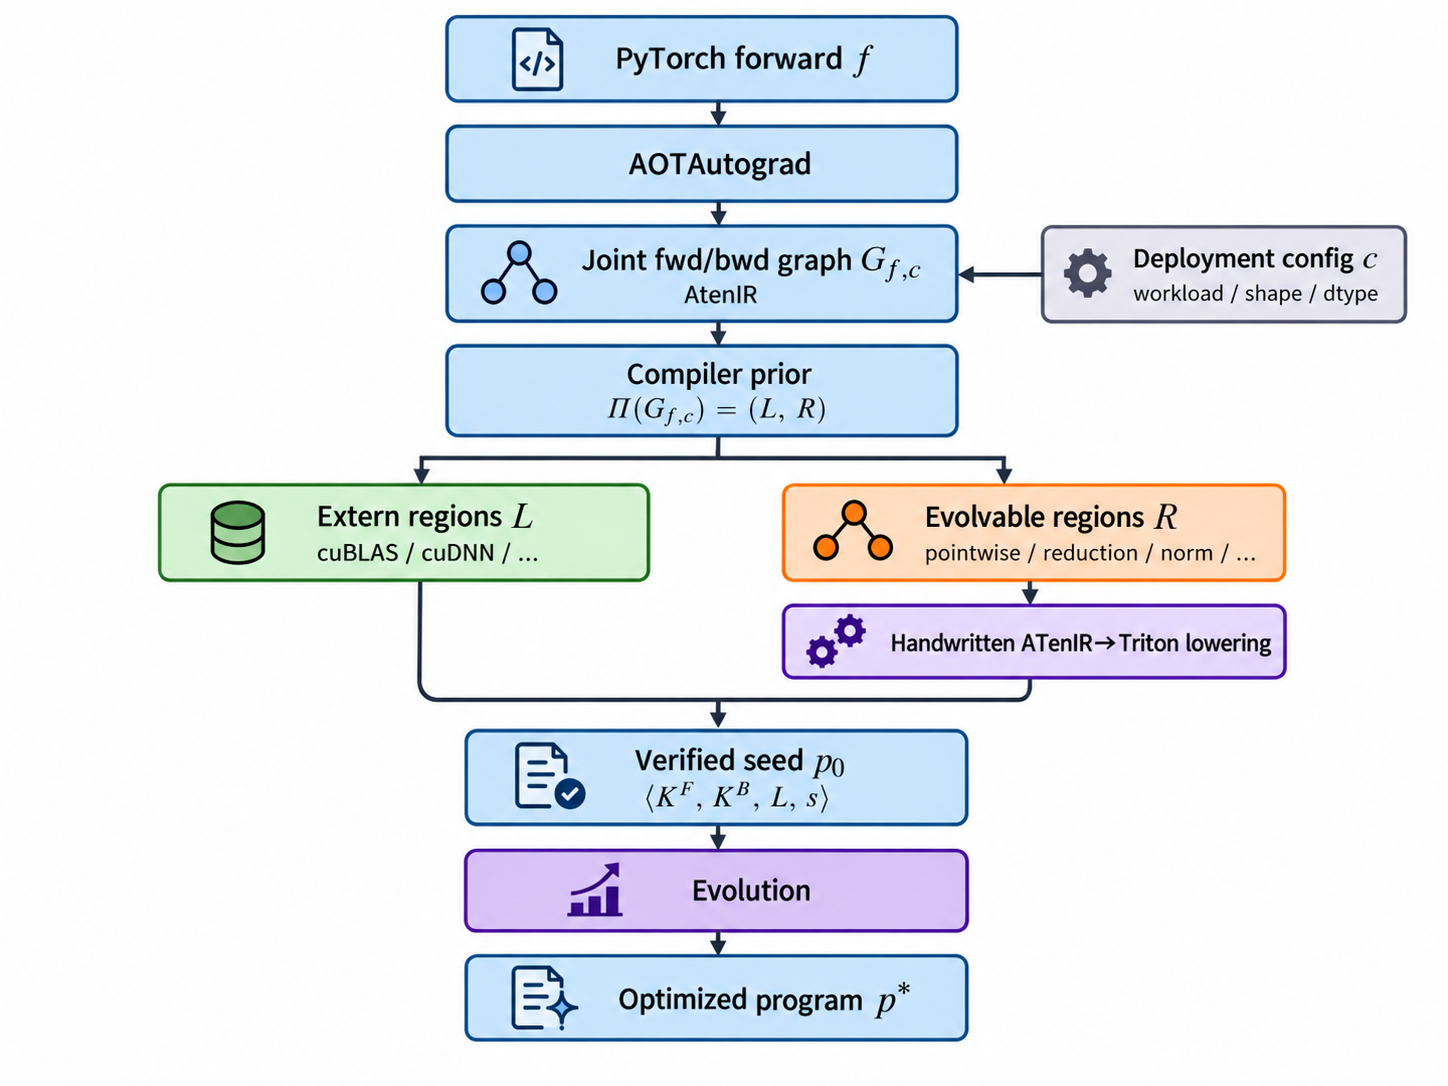
\includegraphics[width=\linewidth]{figures/evograd_pipeline.png}
%     \caption{Overview of \method. AOTAutograd produces a joint forward--backward ATen graph $G_{f,c}$. Compiler-guided partitioning identifies preserved external-library regions $L$ and evolvable semantic regions $R$. Handwritten AtenIR-to-Triton transformations resynthesize $R$, and the resulting kernels are combined with $L$ to form the seed program $p_0$. Evolution jointly optimizes the generated forward and backward implementations and their saved-state policy, with $L$ held fixed.}
%     \label{fig:evograd_pipeline}
% \end{figure}

% \subsection{Compiler-Aware AtenIR Seed Synthesis}
% \label{sec:seed_synthesis}

% \paragraph{Autograd semantic extraction.}
% Given a user-provided PyTorch forward function, \method uses AOTAutograd to derive the corresponding forward and backward computation under deployment configuration $c$. We represent this computation through AtenIR, a graph of ATen operators such as \texttt{aten.add}, \texttt{aten.sum}, and \texttt{aten.mm}. AtenIR captures the required ATen operations and their data dependencies without committing to kernel boundaries or schedules. We initialize the saved-state interface by applying PyTorch's \texttt{min\_cut\_rematerialization\_partition} to the AOTAutograd joint graph, while allowing the saved-state policy to change during subsequent evolution.

% \paragraph{Compiler-aware partitioning.}
% Not every region of the computation should be resynthesized. \method inspects TorchInductor's lowering decisions and partitions the joint graph as
% \begin{equation}
%     \Pi(G_{f,c}) = (L,R),
%     \label{eq:partition}
% \end{equation}
% where $L$ contains regions mapped to external vendor implementations and $R$ contains the remaining computation. In particular, computations such as standard dense GEMMs and convolutions can remain backed by mature libraries such as cuBLAS and cuDNN, avoiding unnecessary search over implementations that are already highly optimized.

% \paragraph{Semantic resynthesis.}
% For the evolvable region $R$, \method returns to its AtenIR representation rather than directly adopting the Triton kernels generated by Inductor. Handwritten lowering rules map supported AtenIR operations to pre-implemented Triton primitives and generate host-side code that invokes them according to the graph's data dependencies. Together, the primitives and their host-side helpers implement the required operator semantics, including broadcasting, dtype conversion, and reduction behavior. This process deterministically constructs a runnable starting point without LLM-based synthesis or cross-operator fusion. These primitive boundaries initialize the seed but remain open to rewriting during evolution. The synthesized forward and backward kernels are then combined with the preserved external-library regions to construct an initial autograd-compatible program
% \begin{equation}
%     p_0 =
%     \left\langle
%         K_0^F,\,
%         K_0^B,\,
%         L,\,
%         s_0
%     \right\rangle,
%     \label{eq:seed_program}
% \end{equation}
% where $K_0^F$ and $K_0^B$ denote the synthesized forward and backward kernels together with their host-side orchestration, $L$ denotes preserved external-library calls, and $s_0$ denotes the state passed from forward to backward. Appendix~\ref{app:seed_example} illustrates the resulting seed
% using a masked linear map, showing the preserved library calls,
% synthesized Triton computation, and forward--backward saved-state interface. 

% \subsection{Evolutionary Optimization}
% \label{sec:evolution}

% Starting from the verified seed $p_0$, \method uses OpenEvolve
% to optimize the objective in Equation~\ref{eq:objective}.
% The search can modify the synthesized Triton kernels,
% their host-side orchestration, and the saved-state policy,
% while preserving the compiler-selected external-library calls
% and public autograd interface. Candidates undergo search-time
% correctness checks before performance measurement; those that
% fail are rejected, while valid candidates receive the fitness
% score defined in Equation~\ref{eq:score} to guide subsequent search.
% Selected final candidates undergo the applicable verification
% and evaluation stages defined by \bench.

% \begin{figure*}[t]
%     \centering
%     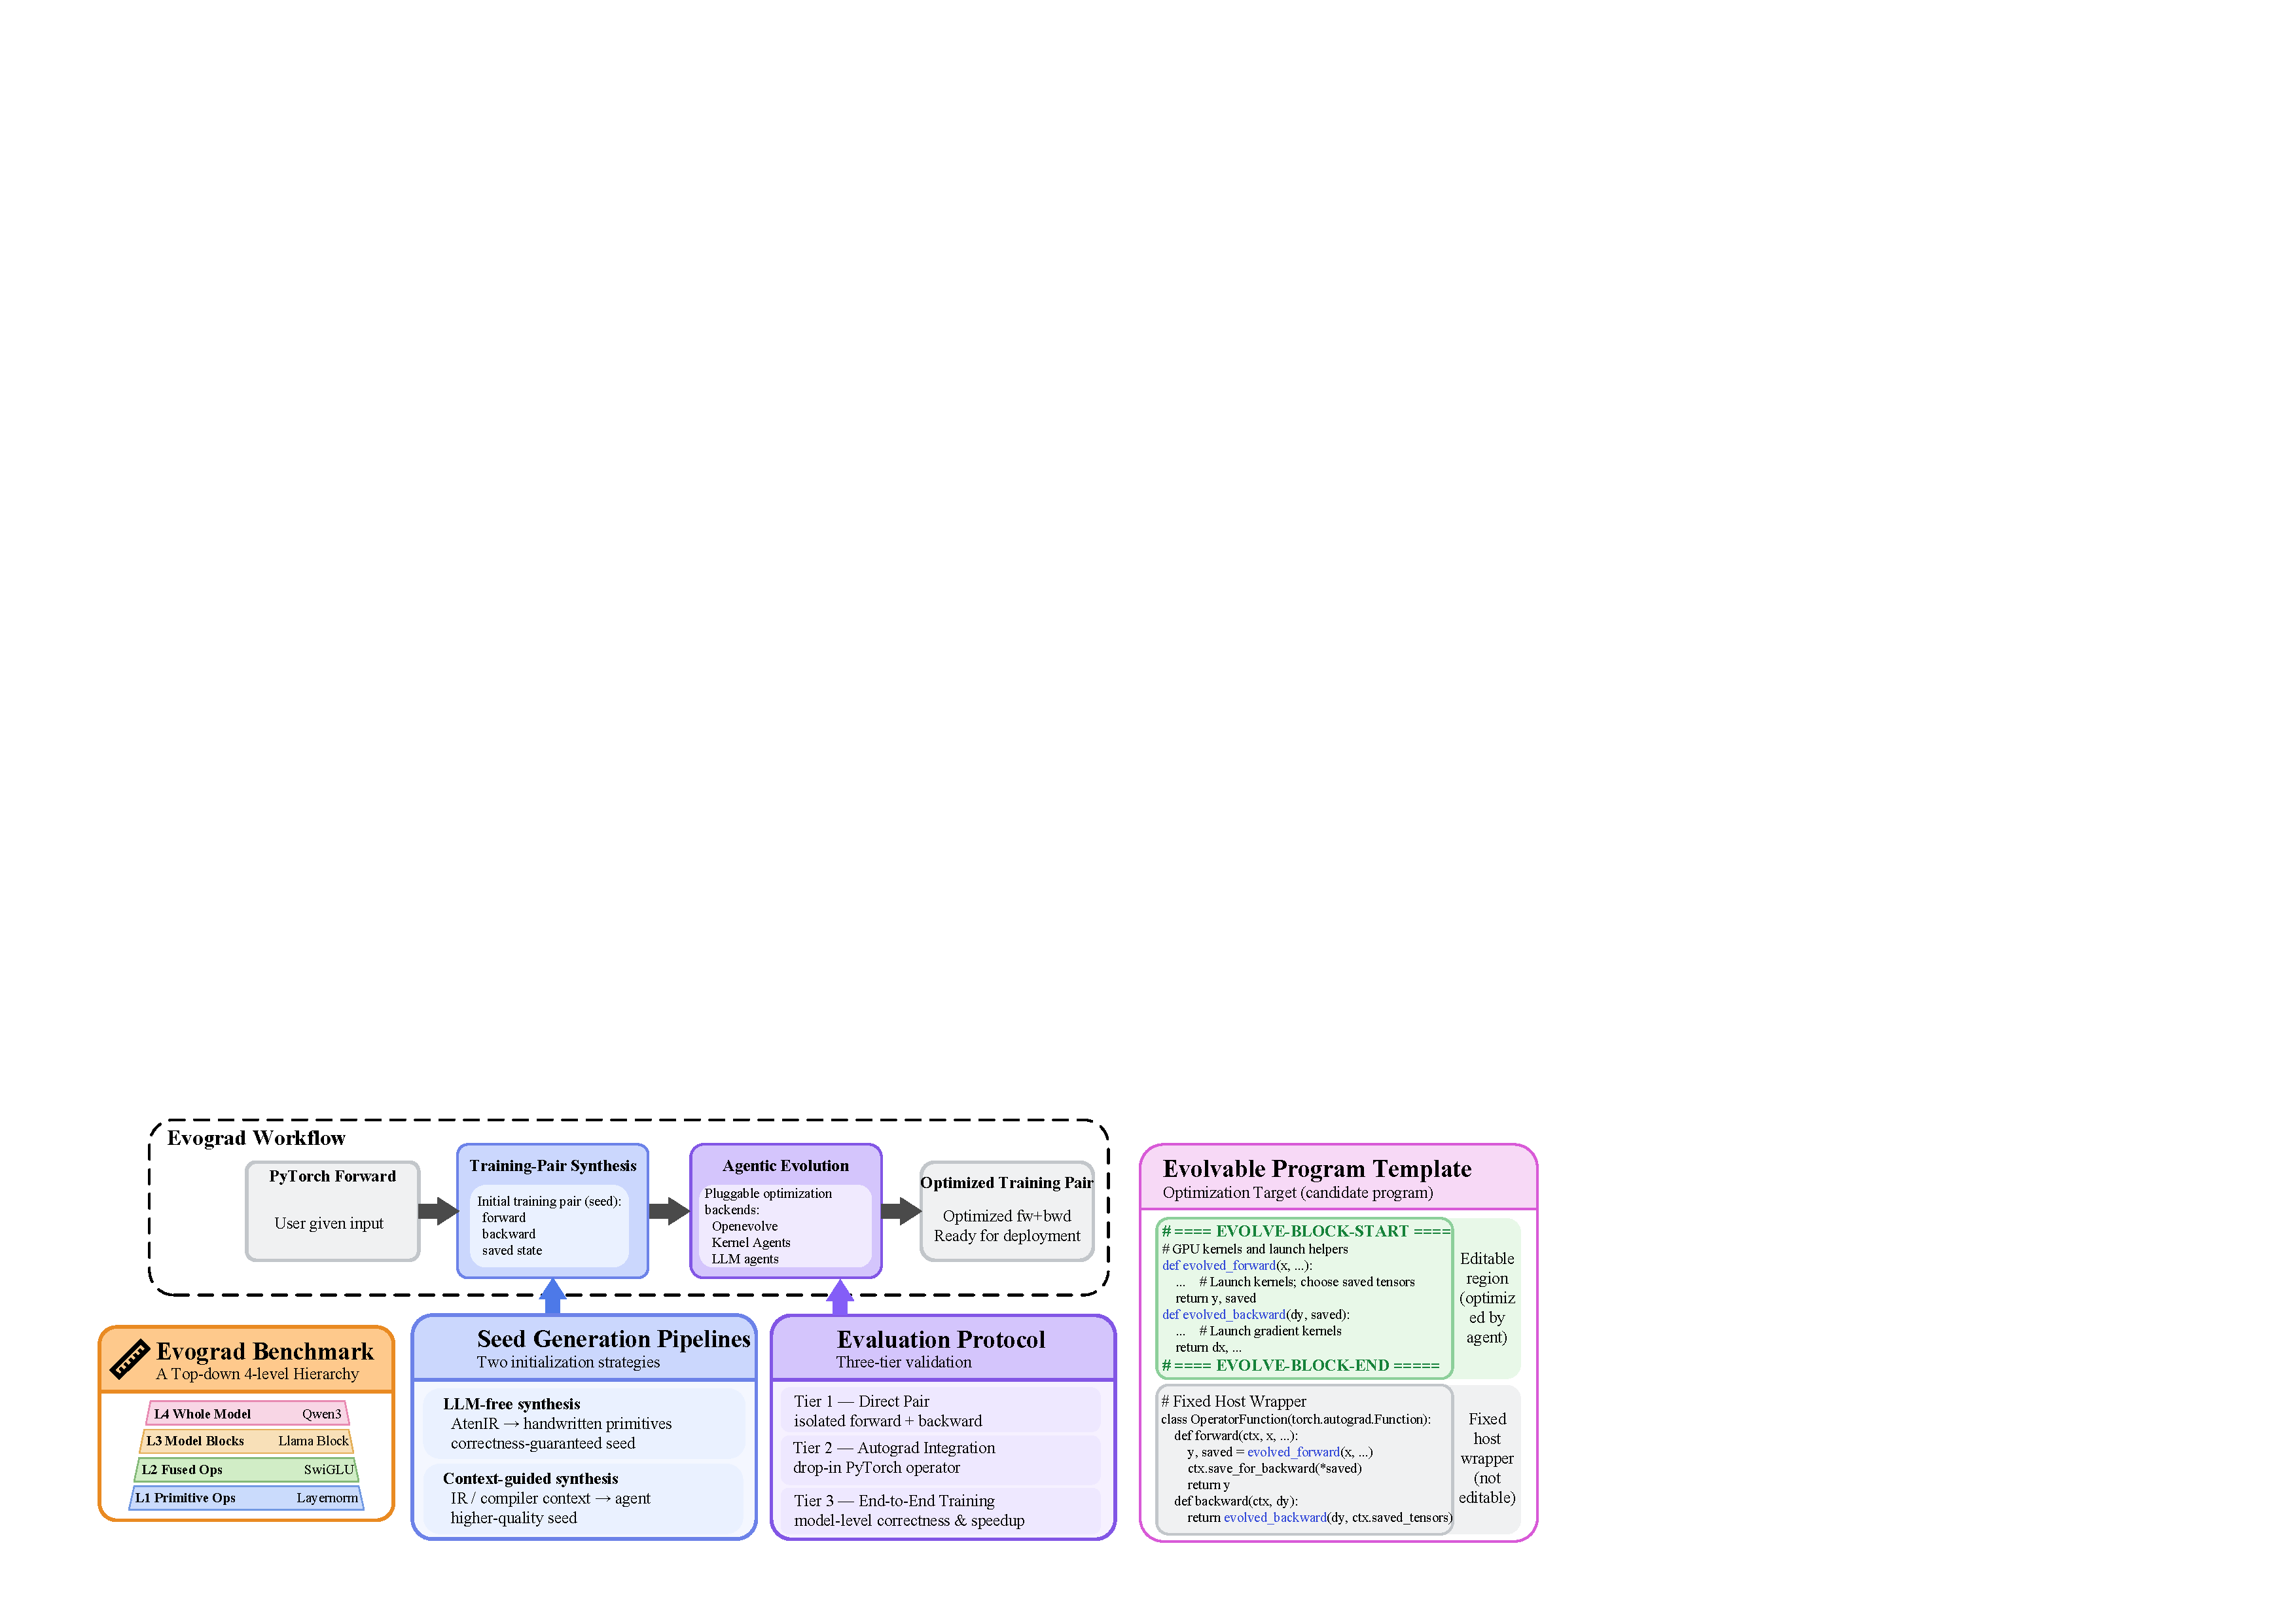
\includegraphics[width=\textwidth]{figures/overview_910.pdf}
%     \caption{Overview of our system. \ahan{Some feedback. (1) Currently each box just states, via words, what is going on. I find this unimformative. We need to diagramatically show, in each box, what is going on. To give a concrete example for agentic evolution we can show some starting code snippet then an ellipses ``..." some intermediate code-snippet showing that it has changed (this is just an example to show how, rather than state what, we are doing). In fact we can show an entry code-snippet in pytorch and show how it is changed in each step, this may be more informative compared to just using words. (2) I am not a big fan of this color scheme, can we use darker colors. (3) You can use the paper X-MoE as a reference: https://arxiv.org/pdf/2508.13337 (See figure 5 for what I mean).} }
%     \label{fig:overview}
% \end{figure*}

% \begin{figure*}[t]
%     \centering
%     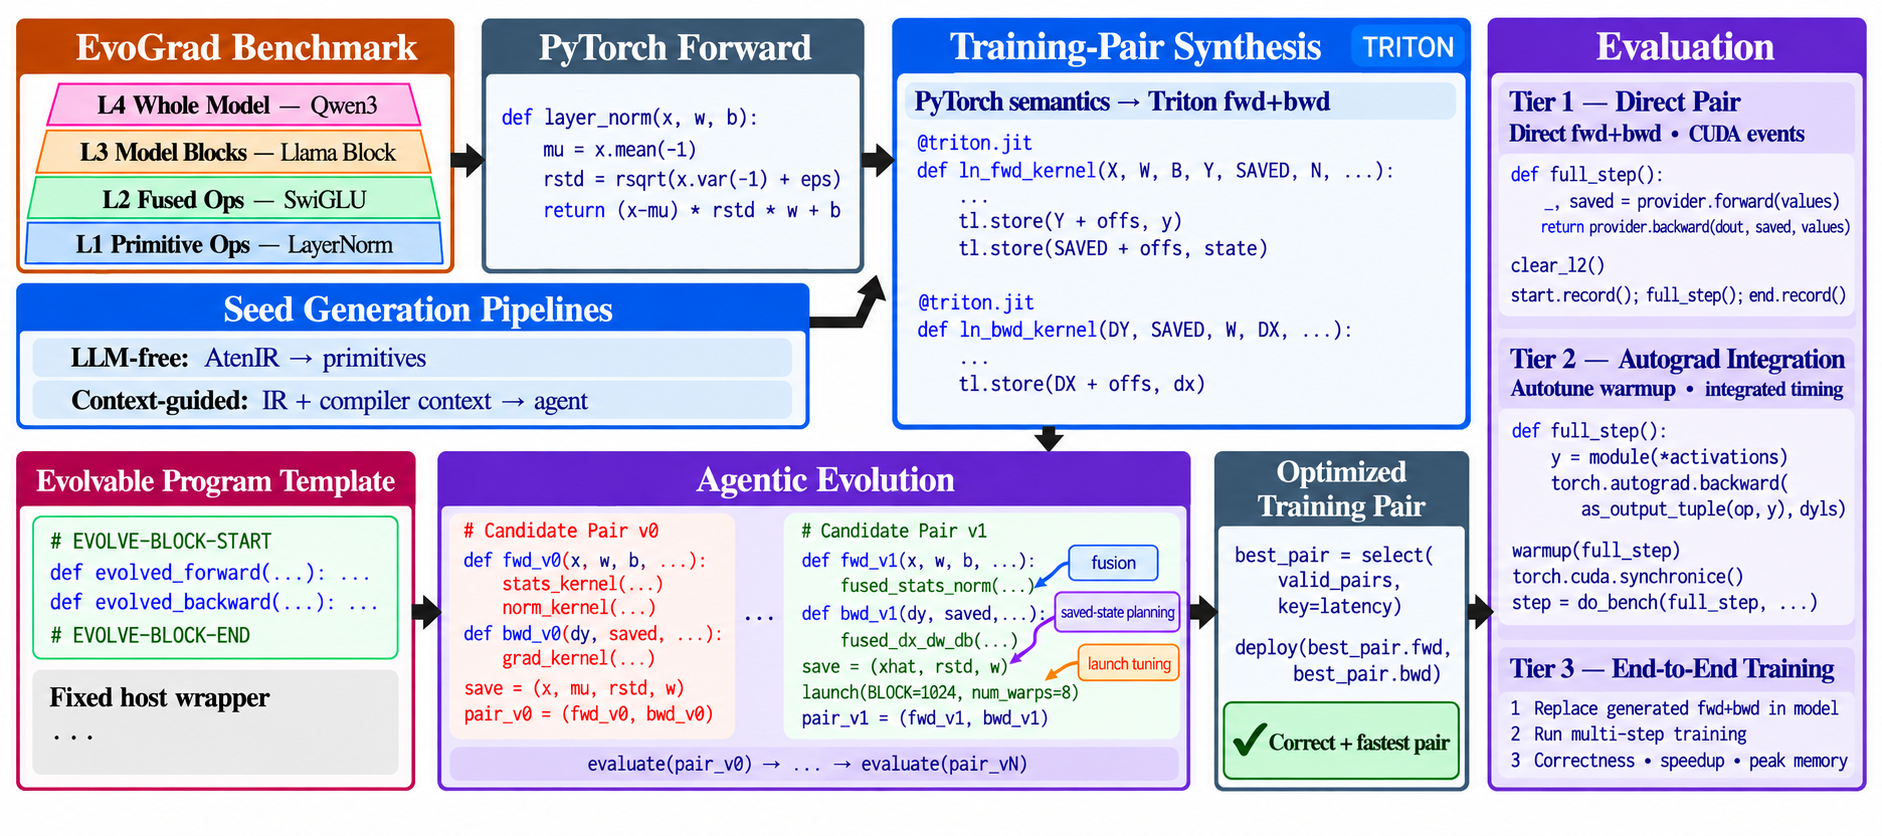
\includegraphics[width=\textwidth]{figures/new_overview.png}
%     \caption{Overview of our system.}
%     \label{fig:overview}
% \end{figure*}

% \ahan{As it's written write now. It's unclear why EvoGrad is needed. The flow introduces ADBench, however, does not state anything as to the problems it exposes. It would be nice to say something like ``hey, now that we've established this benchmark, existing methods sort of suck at AD, spedning many cycles just generating correct programs, resulting in low performance".} \haochen{Word description of the agent benchmarking results. Detailed results are in experiemnt section. }
% Given a task $(f,c)$ specified in Section~\ref{sec:benchmark-task}, \method searches the permitted implementation space $\mathcal{P}_{f,c}$ using a fitness function that combines execution performance and saved-state memory. Candidates remain subject to the forward--backward contract and verification requirements defined by \bench.

% \paragraph{Performance fitness.}
% Let $T_p^{\mathrm{bwd}}(c)$ and $T_p^{\mathrm{full}}(c)$ denote the backward-only and complete forward--backward execution times of candidate $p$, respectively, with $T_{\mathrm{base}}^{\mathrm{bwd}}(c)$ and $T_{\mathrm{base}}^{\mathrm{full}}(c)$ denoting the corresponding performance-baseline times. We define the effective speedup as
% \begin{equation}
%     r(p;c) =
%     \min\!\left(
%         \frac{T_{\mathrm{base}}^{\mathrm{bwd}}(c)}
%              {T_p^{\mathrm{bwd}}(c)},
%         \frac{T_{\mathrm{base}}^{\mathrm{full}}(c)}
%              {T_p^{\mathrm{full}}(c)}
%     \right).
%     \label{eq:effective_speedup}
% \end{equation}
% Using the minimum prevents gains in one execution mode from masking a regression in the other within the performance term.

% \paragraph{Memory penalty.}
% We normalize the logical size of tensors retained for backward by the size of the task's declared memory inputs, defining $R_{\mathrm{saved}}(p;c)=M_p^{\mathrm{saved}}(c)/M_{\mathrm{input}}(c)$. The candidate's fitness is
% \begin{equation}
%     \operatorname{Score}(p;c)
%     =
%     \frac{r(p;c)}
%          {1+\lambda R_{\mathrm{saved}}(p;c)},
%     \label{eq:score}
% \end{equation}
% where $\lambda \geq 0$ controls the penalty for saved memory. This score balances computational speedup against the state retained for backward, allowing recomputation and caching strategies to be compared under the same objective.

% \paragraph{Search objective.}
% The optimization objective is
% \begin{equation}
%     p^\star
%     \in
%     \operatorname*{arg\,max}_{p\in\mathcal{P}_{f,c}}
%     \operatorname{Score}(p;c)
%     \quad \text{subject to} \quad
%     \mathcal{V}(p,f,c)=1,
%     \label{eq:objective}
% \end{equation}
% where $\mathcal{V}$ is the complete verification predicate defined in Eq.~\eqref{eq:validity}. Starting from a seed implementation, \method uses LLM-generated transformations and evaluation feedback to approximate this objective. Search-time checks screen candidates before fitness evaluation; selected candidates must complete the remaining deployment and integration gates before final acceptance. We next describe how \method constructs seeds and organizes candidate transformations.

% \paragraph{Seed structure.}
% Listing~\ref{lst:seed_code_example} illustrates these components using a masked linear map $f(X,W,M)=(XW)\odot M$, where $M$ is a nondifferentiable mask. In the illustrated configuration, the compiler assigns the forward GEMM and the two backward GEMMs to external implementations, forming $L$, while the elementwise multiplications belong to $R$. The same handwritten multiplication primitive is reused by the forward and backward computations. The external-library wrappers and the outer autograd adapter remain fixed, while the primitive kernels, their launch helpers, and the forward--backward orchestration are evolvable. Evolution can therefore replace the initial primitive calls with new implementations and revise the saved-state policy without changing the public autograd interface.


% \ahan{This code listing, though a good start, is too detailed. You don't need to stick to pure Python syntax, you can make it more conscise and readable if you deviate slightly from it.}
% \begin{lstlisting}[
%     language=Python,
%     basicstyle=\ttfamily\scriptsize,
%     columns=fullflexible,
%     keepspaces=true,
%     showstringspaces=false,
%     breaklines=true,
%     frame=single,
%     captionpos=b,
%     caption={Illustrative seed for $f(X,W,M)=(XW)\odot M$. The external-library implementation and autograd adapter are fixed; the Triton primitive, launch helper, and forward--backward orchestration are evolvable. The three preserved GEMM call sites share one displayed wrapper for compactness. Configuration checks and per-region preservation metadata are omitted.},
%     label={lst:seed_code_example}
% ]
% import torch
% import triton
% import triton.language as tl
% from torch._inductor.select_algorithm import extern_kernels

% # Fixed external-library implementation: L.
% def library_mm(a, b):
%     with torch.no_grad():
%         out = torch.empty(
%             (a.shape[0], b.shape[1]),
%             device=a.device, dtype=a.dtype,
%         )
%         extern_kernels.mm(a, b, out=out)
%         return out

% # EVOLVE-BLOCK-START

% # Initial handwritten Triton multiplication primitive.
% @triton.jit
% def _mul_kernel(A, B, OUT, N, BLOCK: tl.constexpr):
%     offsets = tl.program_id(0) * BLOCK + tl.arange(0, BLOCK)
%     mask = offsets < N
%     a = tl.load(A + offsets, mask=mask, other=0.0)
%     b = tl.load(B + offsets, mask=mask, other=0.0)
%     tl.store(OUT + offsets, a * b, mask=mask)

% # Lowering: aten.mul -> host helper -> Triton kernel.
% def mul_tt(a, b):
%     dtype = torch.result_type(a, b)
%     a, b = torch.broadcast_tensors(a, b)
%     a = a.to(dtype).contiguous()
%     b = b.to(dtype).contiguous()
%     out = torch.empty_like(a)
%     grid = (triton.cdiv(out.numel(), 256),)
%     _mul_kernel[grid](a, b, out, out.numel(), BLOCK=256)
%     return out

% # Evolvable forward orchestration and saved state.
% def forward_with_saved(x, w, mask):
%     z = library_mm(x, w)             # Preserved L.
%     y = mul_tt(z, mask)              # Lowered R.
%     return y, (x, w, mask)

% # Evolvable backward orchestration.
% def backward_from_saved(dy, saved):
%     x, w, mask = saved
%     dz = mul_tt(dy, mask)            # Lowered R.
%     dx = library_mm(dz, w.t())       # Preserved L.
%     dw = library_mm(x.t(), dz)       # Preserved L.
%     return dx, dw

% # EVOLVE-BLOCK-END

% # Fixed host adapter for PyTorch autograd.
% class MaskedLinearFunction(torch.autograd.Function):
%     @staticmethod
%     def forward(ctx, x, w, mask):
%         y, saved = forward_with_saved(x, w, mask)
%         ctx.save_for_backward(*saved)
%         return y

%     @staticmethod
%     def backward(ctx, dy):
%         dx, dw = backward_from_saved(dy, ctx.saved_tensors)
%         return dx, dw, None          # No gradient for mask.

% def masked_linear(x, w, mask):
%     return MaskedLinearFunction.apply(x, w, mask)
% \end{lstlisting}

% Before entering evolution, the complete seed $p_0$ is checked against the independent PyTorch-autograd oracle under the same deployment configuration. Only seeds satisfying Equation~\ref{eq:validity} are admitted to the optimization stage.

% \subsection{Profiling-Guided Evolution}
% \label{sec:evolution}

% Starting from the verified seed $p_0$, \method uses OpenEvolve to search for higher-performing programs under the objective in Equation~\ref{eq:objective}. Evolution modifies the synthesized portions of the program while preserving the external-library regions identified during seed synthesis. Each generated candidate must first satisfy the same correctness constraint before its performance is considered.

% The default evolutionary loop uses measured execution performance as its optimization signal. To provide more actionable feedback than a scalar score alone, \method periodically profiles promising candidates with NVIDIA Nsight Compute. A lightweight analysis first identifies major hardware bottlenecks, such as insufficient parallelism, limited memory throughput, or low compute utilization. Selected profiling metrics, together with the current program and deployment context, are then provided to an optimization agent to propose a targeted transformation.

% The proposed program is evaluated using the same correctness and performance gates as ordinary evolutionary candidates. If it improves the objective, it is returned to the OpenEvolve population and becomes available for subsequent search. In this way, profiling feedback supplements broad evolutionary exploration with hardware-specific optimization guidance while leaving correctness and candidate selection under executable evaluation.


% \subsection{Remaining Design Questions}

% \paragraph{Seed-synthesis ablation.} We need an ablation to validate the design choice behind our compiler-aware AtenIR seed synthesis. As discussed, we should compare against two alternative paths: (1) directly evolving compiler-generated Inductor kernels, and (2) synthesizing from AtenIR without compiler-aware partitioning. These comparisons can help isolate the benefit of preserving strong compiler decisions while retaining semantic-level freedom for the remaining computation.

% \paragraph{Evolution agent.} The current draft only describes profiling-guided evolution at a high level. We still need to specify how the evolution agent consumes execution and profiling feedback, identifies optimization opportunities, proposes program transformations, and interacts with the OpenEvolve population. In particular, we should distinguish the hard constraints that every candidate must satisfy from the optimization opportunities that the agent is encouraged to explore.

% \paragraph{Integrating benchmark feedback into optimization.} We also plan to connect the benchmark hierarchy more directly to the optimization framework. For higher-level workloads such as Level-3 cases, instead of synthesizing the entire workload from scratch, we may first optimize lower-level components and compose the higher-level case from these optimized building blocks. Conversely, higher-level evaluation can provide feedback to lower-level optimization. Our current evolution loop is primarily guided by direct forward--backward measurements from Tier-1 evaluation, but the final objective is end-to-end training performance. We should therefore investigate whether Tier-3 signals, such as end-to-end training latency and model-level correctness, can be fed back into evolution for an additional optimization stage targeted directly at deployment-level performance.

% \subsection{Evolution Seed Synthesis}

% \ahan{Another question while reading this. PyTorch-2 inductor automatically code-generates Triton. Why don't we just use those kernels and evolve those rather than do this whole Aten-IR based code-gen? Do we want to motivate why we're doing it this way instead? I see that you compare against naive LLM generated forward baseline, but perhaps we want to talk about this? Just a thought.} \haochen{Added a discussion for this. The pytorch-2 seed generation pipeline is introduced here, while the ablation results are included in 7.}


% \haochen{One thing I'm not sure about the outline of 4.2 and 4.3 is that whether we should include all the methods / agentic frameworks we studied here, or include them in ablations in section 7. I think a reasonable arrangement in my perspective is to include the one final pipeline (after we made the decision) in section 4 along with its advantage, and move the discussions of other possible solutions to section 7. Right now in 4.2 we included all possible ways to do seed synthesis. Please correct me if I misunderstood. }
% \minjia{Yes, we only show the best performing solution in the design. If some components are inspired by other work, we make it explicit. Then we can conduct ablation studies in the evaluation analysis section to show the importance of those components. }

% We explored two different pipelines to generate the initial program for the evolving agent to improve on. In the agent-guided pipeline, a compact summary of the backward AtenIR graph is provided to an LLM that generates a fused Triton seed. This pipeline is flexible, but correctness is not guaranteed and may require multiple generate–evaluate–repair iterations, increasing token and search cost. In the llm-free pipeline, we hand-write and verify Triton kernels for a supported set of ATen operators, then compose these kernels according to the AtenIR data dependencies. This produces a correctness-guaranteed, initially unfused backward seed. Beyond avoiding the repair loop, the structured seed provides evolution with a reliable starting program and reduces the risk of premature convergence to a poor local optimum.

% \subsection{Evolving Agent}
% \subsection{Shape Dispatch}

% \method builds on OpenEvolve as the underlying search engine and augments
% score-based evolution with hardware profiling feedback. Every few iterations, we use the profiling results to optimize the current evolved kernel. A lightweight deterministic roofline analysis first classifies the
% kernel as underutilized, memory-bound, or compute-bound using SM and DRAM
% throughput. Only candidates with meaningful optimization headroom are passed to
% an analysis agent, which combines the roofline result, selected NCU metrics,
% GPU specifications, and benchmark context to produce structured bottleneck
% diagnoses and concrete optimization suggestions. A generation agent then
% revises the program under fixed interface and saved-tensor constraints, so the
% profiling feedback guides performance optimization without changing the task
% contract. The optimized kernel, if scores higher than the origin kernel, would silently replace the original kernel in OpenEvolve's candidate pool to fuel future free exploration. 

% \method treats input shape as a first-class optimization dimension. It
% separately evolves specialists for small and large shapes, evaluates the
% resulting candidates over the full deployment grid, and selects a contiguous
% dispatch threshold from measured performance. The final output is a single
% all-in-one program that dispatches to the appropriate specialist at runtime.
% Our current LayerNorm experiments show that two shape regimes capture most of
% the available gain over a single mixed-shape implementation, while introducing
% a third regime yields only limited additional benefit.






% \section{Benchmark Design}
% \section{Model Workloads and Target Operators}
\section{\system-Bench}
\label{sec:workloads}
% \ahan{We cannot directly talk about our benchmark. There needs to be sufficient buildup and motivation. We need to motivate why our benchmark is necessary: i.e. what does it plug in the existing literature that other benchmarks do not consider?}\wangjia{done.}

\minjia{Please restructure Section 4 as ADopt-Bench. The current section reads more like workload preparation for our experiments than an independent benchmark contribution. Please look at the intro to see how ADopt-bench is introduced and its position in the paer. We should explain what makes ADopt-Bench different from existing kernel benchmarks, and how each task incorporates its training and deployment context. Make the task specification, model and operator coverage, submission interface, and assessment protocols explicit. A reader should understand how to use ADopt-Bench to evaluate their own kernel agents without relying on ADopt's seed synthesizer or evolver. 1-1.5 pages.}

We prepare primitive and composite kernel targets together with model-training workloads to instantiate $\mathcal I=(\mathcal O,M,W)$. The operators define the kernel-optimization tasks; each model and its declared training setup provide the context for model-level verification and evaluation. Two principles guide preparation: training kernels are assessed as forward--backward implementations, and their configurations come from the workloads in which they are deployed. Calls recorded from source models running on real datasets support operator verification and timing. Candidates are assessed through their autograd interfaces and, where supported, within those models. Figure~\ref{fig:workload_overview} summarizes the prepared workload categories. We next describe the target operators, workload-derived configurations, and experimental selections.

\begin{figure}[h]
    \centering
    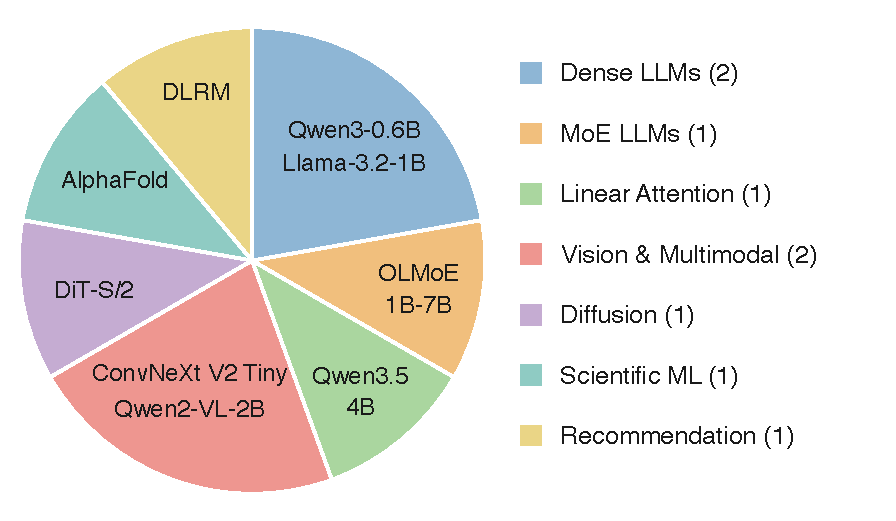
\includegraphics[width=\linewidth]{figures/benchmark_overview.pdf}
    \caption{Prepared models across seven workload categories. Numbers indicate the number of model workloads in each category. }
    \label{fig:workload_overview}
\end{figure}

% \noindent\textbf{Performance and saved memory.} 
% \bench measures execution time and the logical size of tensors retained in $s_p$ for backward to characterize compute--memory tradeoffs. Whole-model evaluation also reports peak allocated GPU memory. Section~\ref{sec:evaluation_protocol} defines the measurement scopes, speedups, and memory accounting.

% \subsection{Model-Driven Benchmark Construction}
\subsection{Target Operators and Workload Preparation}
\label{sec:target_preparation}
\label{sec:workload_configs}
For our experiments, we select kernel targets from prepared model-training workloads. Starting from a source model, we identify computations that form meaningful kernel-optimization boundaries and record their model sites for verification and evaluation. For each source model, we fix the training workload and extract tensor shapes, dtypes, memory layouts, and static operator parameters from forward--backward execution. Calls sharing the same reference computation and configuration form one kernel task, whose manifest records model locations and call counts so that repeated calls across layers do not create duplicate tasks. These targets comprise primitive and composite operators.

\noindent\textbf{Primitive operators.}
Primitive targets include reusable computations such as normalization, activation, reduction, loss, matrix multiplication, convolution, positional encoding, and attention. Each task specifies a PyTorch forward computation and its required gradients, evaluating the generation and optimization of a single autograd-compatible operator.

\noindent\textbf{Composite operators.}
Composite targets group adjacent computations that form a meaningful optimization target in a model's training path, such as linear projection followed by activation, residual addition followed by normalization, or attention computations that span multiple primitive operations. These tasks expose optimization opportunities across operator boundaries, including fusion, elimination of intermediate global-memory traffic, and joint forward--backward implementation choices.
% We use the term \emph{composite operator} rather than \emph{fused operator}: the benchmark defines the computation that must be implemented, while fusion remains an implementation choice available to the system being evaluated.

\noindent\textbf{Training execution.}
Each workload specifies complete model-training execution, including forward computation, loss computation, backward propagation, optimizer update, and gradient reset. Supported optimized implementations are installed at their corresponding operator boundaries throughout the model, where they execute alongside the remaining model computation and framework overhead. Model-scope evaluation measures their effect on end-to-end training time and peak allocated GPU memory.

Primitive and composite targets expose the computations available for kernel synthesis and evolution. The supplied model workload provides the context for deployment verification and measurement of training time and memory. The system returns optimized kernel implementations with their deployment bindings.

% \subsection{Workload-Driven Configurations}
% \label{sec:benchmark_workloads}
% We instantiate the tasks of each source model top-down from an explicitly specified training workload. Standalone operator benchmarks, such as those in Liger-Kernel~\cite{hsu2024liger}, evaluate kernels over predefined shape sweeps; our tasks additionally retain their source-model and training contexts. For each source model, we fix the architecture, batch size, input extent, data type, and execution backend, which determine the operator configurations, and the training data used by the workload (Table~\ref{tab:benchmark_composition}).

% \noindent\textbf{Configuration extraction.}
% We execute a forward--backward pass and record tensor shapes, dtypes, memory layouts, and static operator parameters at the Level~1--2 boundaries defined in Section~\ref{sec:benchmark-hierarchy}. Calls to the same reference computation under equivalent configurations form one task; different configurations form separate tasks. The workload manifest records each task's source model, workload settings, model locations, and call count, so repeated calls across layers increase its frequency without creating duplicate tasks.


\subsection{Prepared Workloads and Target Configurations}
\label{sec:workload_composition}

Table~\ref{tab:workload_composition} summarizes the prepared source models, workload data, precision settings, and available primitive/composite configurations. Section~\ref{sec:results} reports a subset of these workloads and targets. Detailed configurations and experimental selections appear in \appref{app:operator_configs}.

\begin{table}[t]
\centering
\caption{Prepared model workloads and operator configurations. P and C count primitive and composite configurations; M counts model workloads. Mixed denotes FP32 with BF16 autocast.}
\label{tab:workload_composition}
\begingroup
\small
\setlength{\tabcolsep}{3pt}
\renewcommand{\arraystretch}{1.05}
\begin{tabularx}{\columnwidth}{@{}Xlcrrr@{}}
\toprule
\textbf{Model}
& \textbf{Workload data}
& \textbf{dtype}
& \textbf{P}
& \textbf{C}
& \textbf{M} \\
\midrule

\multicolumn{6}{@{}l}{\emph{Dense LLMs}} \\
Qwen3-0.6B & WikiText-2 & BF16 & 14 & 4 & 1 \\
Llama-3.2-1B & WikiText-2 & BF16 & 11 & 4 & 1 \\

\multicolumn{6}{@{}l}{\emph{MoE LLMs}} \\
OLMoE-1B-7B & WikiText-2 & BF16 & 8 & 4 & 1 \\

\multicolumn{6}{@{}l}{\emph{Linear attention}} \\
Qwen3.5-4B & WikiText-2 & BF16 & 20 & 7 & 1 \\

\multicolumn{6}{@{}l}{\emph{Vision and multimodal}} \\
ConvNeXt V2-Tiny & Imagenette & BF16 & 31 & 4 & 1 \\
Qwen2-VL-2B & TextVQA & BF16 & 16 & 2 & 1 \\

\multicolumn{6}{@{}l}{\emph{Diffusion}} \\
DiT-S/2 & Imagenette & FP32 & 10 & 2 & 1 \\

\multicolumn{6}{@{}l}{\emph{Scientific ML}} \\
MegaFold (AF3) & PDB & Mixed & 2 & 2 & 1 \\

\multicolumn{6}{@{}l}{\emph{Recommendation}} \\
DLRM & Criteo Kaggle & FP32 & 7 & 1 & 1 \\

\midrule
\textbf{Total} & & & \textbf{119} & \textbf{30} & \textbf{9} \\
\bottomrule
\end{tabularx}
\endgroup
\end{table}

These model-derived tasks connect the framework's implementation search to the training contexts in which its outputs are assessed. Section~\ref{sec:results} evaluates a subset of 18 primitive cases, 17 composite cases, and six prepared model workloads.

% Compact Tier-3 results.
\begin{table*}[t]
\centering
\caption{Whole-model training results with selected kernels deployed jointly. Speedup and peak memory are relative to eager; / denotes no qualifying combination, and -- denotes unavailable data.}
\label{tab:agent_tier3_results}
\footnotesize
\setlength{\tabcolsep}{2pt}
\begin{tabular}{@{}l cc cc cc cc cc cc@{}}
\toprule
 & \multicolumn{2}{c}{\texttt{torch.compile}$^{\mathrm{GH200}}$}
 & \multicolumn{2}{c}{\textbf{evograd (ours)}$^{\mathrm{A100}}$}
 & \multicolumn{2}{c}{OpenEvolve}
 & \multicolumn{2}{c}{GEPA}
 & \multicolumn{2}{c}{KernelAgent$^{\mathrm{A100}}$}
 & \multicolumn{2}{c}{Codex} \\
\cmidrule(lr){2-3} \cmidrule(lr){4-5} \cmidrule(lr){6-7}
\cmidrule(lr){8-9} \cmidrule(lr){10-11} \cmidrule(lr){12-13}
Benchmark (L3) & Spd. & Mem & Spd. & Mem & Spd. & Mem
 & Spd. & Mem & Spd. & Mem & Spd. & Mem \\
\midrule
Llama-3.2-1B & 1.13 & 0.77 & 1.033 & 1.00 & 1.11 & 0.95 & 1.11 & 0.95 & / & / & 1.11 & 0.85 \\
Qwen3-0.6B & 1.66 & 0.67 & 1.108 & 0.88 & 1.15 & 0.95 & 1.35 & 0.90 & / & / & / & / \\
Qwen2-VL-2B & 1.14 & 1.00 & / & / & / & / & / & / & 1.070 & 1.00 & / & / \\
ConvNeXt V2-Tiny & 1.26$^{\ddagger}$ & 0.63$^{\ddagger}$ & 1.119 & 0.83 & / & / & / & / & / & / & 1.06 & 0.98 \\
DiT-S/2 & 1.14 & 0.89 & 1.000 & 1.00 & / & / & 1.00 & 1.00 & / & / & / & / \\
DLRM & 1.13 & 1.00 & 1.005 & 1.00 & 1.05 & 1.00 & 1.03 & 1.00 & 1.007 & 1.00 & 1.04 & 1.00 \\
\midrule
Geo.\ mean & -- & -- & 1.052 & -- & -- & -- & -- & -- & 1.038 & -- & -- & -- \\
\bottomrule
\end{tabular}
\end{table*}

% Results section: three complementary questions.
\section{Experiment Results}
\label{sec:results}

We evaluate forward--backward correctness, deployed operator performance (Tier~2), and full training-step performance (Tier~3) on six workloads. OpenEvolve, GEPA, and Codex run on GH200; EvoGrad and KernelAgent run on A100. Comparisons use baselines on the same device; we do not rank agents across hardware. 


\subsection{Benchmark Results}
\label{sec:cross-tier}

We first ask whether generated kernels accelerate training after integration. Across all five workflows, 28 of 43 accepted L2 agent--case implementations with paired measurements beat eager at Tier~2, but only 17 of these have a Tier~3 confidence interval entirely above one; ten become slower in training. OpenEvolve's DLRM interaction drops from $3.830\times$ locally to $1.055\times$ in training, while its Qwen3 SwiGLU MLP reverses from $1.066\times$ to $0.964\times$. Conversely, KernelAgent's Qwen2-VL text MLP measures $0.490\times$ locally but $1.046\times$ in training. Thus, local speedups do not translate proportionally into training gains and can predict the wrong direction (Table~\ref{tab:tier_transfer_summary}).

\begin{table}[t]
\centering
\caption{Tier-2 gains do not reliably transfer to training. T3+ counts local wins with a training-speedup 95\% CI above one; T3-- counts training slowdowns.}

\label{tab:tier_transfer_summary}
\footnotesize
\setlength{\tabcolsep}{3pt}
\begin{tabular*}{\columnwidth}{@{\extracolsep{\fill}}lrrrr@{}}
\toprule
Agent & Paired & T2+ & T3+ & T3-- \\
\midrule
EvoGrad & 10 & 5 & 5 & 0 \\
OpenEvolve & 11 & 9 & 3 & 6 \\
GEPA & 9 & 7 & 4 & 2 \\
KernelAgent & 3 & 2 & 1 & 1 \\
Codex & 10 & 5 & 4 & 1 \\
\midrule
Total & 43 & 28 & 17 & 10 \\
\bottomrule
\end{tabular*}
\end{table}


Selected combinations improve eager by up to $1.351\times$, yet only two of 11 qualifying combined deployments beat whole-model \texttt{torch.compile}, both from EvoGrad (Table~\ref{tab:agent_tier3_by_model}). Training also exposes latency--memory tradeoffs: EvoGrad's DiT MLP reduces peak memory to $0.84$ of eager while slowing the step to $0.988\times$. These results show why training optimization requires whole-step latency and memory measurements, rather than local speed alone. Missing or correctness-disqualified baselines are excluded from compile comparisons.

\begin{table}[t]
\centering
\caption{Accepted coverage and training performance. Coverage uses 18 L1 cases, 17 L2 cases, and six models. Speedup and memory are geometric means over accepted combinations.}

\label{tab:agent_tier3_results}
\footnotesize
\setlength{\tabcolsep}{2.5pt}
\begin{tabular*}{\columnwidth}{@{\extracolsep{\fill}}lccccc@{}}
\toprule
 & \multicolumn{3}{c}{Coverage (accepted / total)} & & \\
\cmidrule(lr){2-4}
Agent & L1 & L2 & L3 & Spd. & Mem \\
\midrule
EvoGrad & 13/18 & 10/17 & 5/6 & 1.052 & 0.939 \\
OpenEvolve & 12/18 & 11/17 & 3/6 & 1.103 & 0.966 \\
GEPA & 12/18 & 9/17 & 4/6 & 1.116 & 0.962 \\
KernelAgent & 14/18 & 3/17 & 2/6 & 1.038 & 1.000 \\
Codex & 13/18 & 10/17 & 3/6 & 1.071 & 0.940 \\
\bottomrule
\end{tabular*}
\end{table}


\subsection{Failure Analysis}

We next ask where generated implementations fail. The 35 cases across five workflows define 175 planned agent--case evaluations. Of these, 170 have submissions and five have no submission; 107 submissions are accepted, 54 rejected by verification, two violate static rules, and seven have unresolved verdicts. Counting each verification rejection at its first failed gate, 41 fail deployed-operator verification, seven model integration, five payload verification, and one training verification. Of these 54 rejections, 51 exceed numerical tolerances and three are runtime bugs. Deployment correctness, particularly numerical agreement in outputs and gradients, is therefore the dominant rejection boundary (Table~\ref{tab:failure_summary}).

\begin{table}[t]
\centering
\caption{Failure analysis across 35 cases per workflow. Rejections are assigned to the first failed gate; incomplete evaluations and missing submissions are counted separately.}

\label{tab:failure_summary}
\scriptsize
\setlength{\tabcolsep}{2pt}
\begin{tabular*}{\columnwidth}{@{\extracolsep{\fill}}lrrrrrr@{}}
\toprule
Outcome & EG & OE & GEPA & KA & CX & Total \\
\midrule
Accepted & 23 & 23 & 21 & 17 & 23 & 107 \\
G1: payload & 0 & 0 & 2 & 1 & 2 & 5 \\
G2: operator & 8 & 9 & 8 & 9 & 7 & 41 \\
G2: model & 2 & 1 & 2 & 1 & 1 & 7 \\
G3: training & 0 & 1 & 0 & 0 & 0 & 1 \\
Static violation & 0 & 0 & 0 & 2 & 0 & 2 \\
No verdict: OOM & 2 & 0 & 0 & 2 & 0 & 4 \\
No verdict: calibration & 0 & 1 & 1 & 0 & 1 & 3 \\
No submission & 0 & 0 & 1 & 3 & 1 & 5 \\
\midrule
Submitted & 35 & 35 & 34 & 32 & 34 & 170 \\
Planned & 35 & 35 & 35 & 35 & 35 & 175 \\
\bottomrule
\end{tabular*}
\end{table}


Earlier acceptance does not guarantee agreement during training: OpenEvolve's ConvNeXt stage-0 MLP passes operator and model checks but exceeds the training-loss deviation limit ($0.03101$ versus $0.02490$). These failures establish disagreement under the numerical policy, not necessarily training divergence. Evaluation limitations are separate: three ConvNeXt layernorm verdicts lack valid calibration after compile-control failure, and four Llama evaluations lack model-level verdicts because verification runs out of memory.


\subsection{EvoGrad Performance}

EvoGrad achieves the broadest L3 combination coverage, with modest speed gains (Table~\ref{tab:agent_tier3_results}). Its overall accepted coverage is 23/35, tied with OpenEvolve and Codex. At L2, it accepts 10/17 planned cases versus KernelAgent's 3/17 (three accepted from 14 submissions); on their 14 jointly submitted targets, the counts are nine versus three. It produces five accepted combinations versus two, with conditional training-speed geometric means of $1.052\times$ and $1.038\times$ over different model subsets. Its strongest combinations are ConvNeXt ($1.119\times$, memory ratio $0.83$) and Qwen3 ($1.108\times$, $0.88$). EvoGrad also exceeds the reported whole-model compile baseline on Llama and Qwen3 by $1.8\%$ and $1.3\%$.

EvoGrad has no payload-verification rejection or static violation, consistent with more robust construction of deployable pairs. However, ten submissions still fail numerical checks; the results do not establish improved long-term training stability or isolate the contribution of seed synthesis. Its remaining failures and modest end-to-end gains motivate stronger integration verification and model-aware latency--memory objectives during search.
% \section{Ablations}

\haochen{potentially mode into experiment section ? }
\subsection{Seed Synthesis Frontend}
% After the forward kernel is passed in, EvoGrad generates the backward kernel for this specific forward and produces the initial forward--backward pair as the optimization seed. 

% \method exploits AtenIR during seed synthesis in order to capture the computation graph of the backward kernel. AtenIR is a low-level representation of PyTorch programs expressed through
% ATen operators, such as \texttt{aten.add} and \texttt{aten.sum}
% ~\cite{pytorch-aten-ir}. It exposes the backward graph produced by PyTorch
% autograd without committing to a specific CUDA or Triton implementation. 

% \subsubsection{Methods}

 
% A straightforward baseline is to prompt an LLM directly from the forward program alone and iteratively repair the generated backward seed. Our
% earlier experiments show that both AtenIR-based paths improve
% cost efficiency and seed quality: AtenIR grounding reduces the
% number of generate–evaluate–repair iterations, while deterministic lowering produces a correct, unfused, and structured seed that
% provides a stronger starting point for subsequent evolution.


% Our llm-free pipeline guarantees correctness and provides a fully unfused back-ward seed, which gives the evolving agent more space for optimization. 
% However, PyTorch-2 inductor also automatically generates triton kernels for both forward and backward pass when we use
% torch.compile. Compared with our approach, PyTorch-2 provides a
% more optimized starting point through mechanisms like the min-cut
% partitioner.

% \subsubsection{Results}
% \subsubsection{Analysis} 
% The ablation results justify our design choice. 
% First, by comparing the agent-guided pipeline with the AtenIR-free pipeline, we can see that AtenIR backward graph improves initial program performance and reduces evolution variance. By examine the seed, we notice that AtenIR graph typically prevents the forward kernel from over-saving, thus explains the higher initial program performance. 

% Second, by examining the evolution process of PyTorch-2 generated seeds, we conclude that PyTorch-2 generated code is structurally unsuitable for evolution. PyTorch-2 kernels often contain meaningless variable names, structure-oriented function names, compiler-specific comments, and specialized APIs. These characteristics create two major problems. First, they can mislead the agent when modifying the code, resulting in a substantially higher error rate. Second, they make it difficult for the agent to identify which parts of the implementation are actually performance-critical, causing it to waste iterations modifying, fixing, or polishing irrelevant compiler-generated code. Consequently, the agent often abandons the original implementation and writes a simpler kernel from scratch, leaving much of the compiler-generated code orphaned.

\subsection{evolving backend}
\paragraph{geak and gepa}
\paragraph{map-elited with shape}

\paragraph{Ablation: Tier-1 versus Tier-2 search guidance.}
\textbf{TODO.}
Evaluate whether Tier-1 fitness provides additional value over
Tier-2 fitness for kernel evolution. Starting from identical programs
under matched search budgets and controlled feedback, compare both
strategies on representative cases, including Qwen3 QKV--Norm--RoPE
(Level 2). Validate numerical correctness at the benchmark shapes
and evaluate all selected kernels using a shared Tier-2 protocol
across repeated searches. If Tier-1 guidance yields no meaningful
benefit, consider omitting it as a search objective while retaining
the required correctness checks.
\section{Discussion and Conclusion}
We presented \method, a compiler-guided agentic system for optimizing AD kernels. Given target kernels, it jointly synthesizes and optimizes forward computation, backward computation, and their saved-state interface. Users also supply a model and workload configurations for model-level verification and evaluation; \method returns selected kernel implementations and their deployment bindings. Its seed synthesizer exposes compiler-derived training semantics as editable implementations; its evolver explores the joint kernel program space; and its verifier and evaluator connect local optimization to numerical acceptance and training-level deployment selection.

Across five workflows, only 107 of 170 submissions are accepted, and only 17 of 28 accepted implementations with deployed-operator speedups retain statistically supported training gains. \method produces qualifying combined deployments on five of six evaluated workloads, but its end-to-end gains remain modest. These results expose a persistent gap in agentic training optimization: local correctness and speed do not reliably translate into correct, faster training.

Saved-state search is complementary to graph-level activation checkpointing and rematerialization: \method changes the custom forward--backward program and its internal interface, while the surrounding compiler may optimize compiler-visible values. Our results do not isolate the contribution of seed synthesis, establish long-term training stability, or characterize this interaction with subsequent compilation. Designing agentic workflows that directly optimize end-to-end training remains an opportunity for future work.
% \method demonstrates that automatic training-kernel generation is not merely
% a problem of translating a backward formula into Triton. The system must also
% construct an independent correctness contract, choose saved forward state,
% search reduction and fusion strategies, and specialize deployment across
% shape regimes. Our current benchmark schema primarily targets two-dimensional
% row-by-column operators; attention, RoPE, and fused-linear families require a
% more general multi-input and multi-output representation. In addition, task
% self-checking validates contract wiring but does not fully validate numerical
% tolerance calibration, and evolutionary runs still exhibit nontrivial
% variance. Addressing these limitations is necessary for broader automation,
% but the current results show that correctness-constrained evolution with simple
% shape dispatch can already produce robust, high-performance autograd kernels.

% \ahan{Putting down a thought here. Though I like the current challenge. In my opinion another key challenge is the interplay of correctness and optimization. The crux being, EvoGrad must output fundamentally correct kernels by construction (at the end of its optimization "passes"). However, this is challenging to do, because there are no correctness guarantees on the output of LLM code-generation. So we need to design an LLM-in-the-loop strategy that iteratively optimizes kernels in a manner that outputs a correctly code-generated kernel in the end. Another thing about this correctness uniqueness to AD is that the user codes and thinks about and codes the forward pass, whilst the backwards pass is hidden and automatically generated. Thus viable solutions must be generated for llm code-optimization. This uniqueness isn't there in a lot of other LLMs for code-optimization literature in the way its present for us (unless I am incorrect). The added layer of indirection makes this evermore challenging as the seed for LLM input must be code-generated and correct first, prior to optimization. Our design space must necessarily then consist of formal techniques + LLM optimization. This makes our design explicit: a separation of concerns between lowering and optimization, lowering is formal whilst optimization is aided by LLM, giving a ground truth to repeatedly check against. Without making correctness a first class citizen that we explicitly curated a design for, it may be tough to motivate the way we do things in EvoGrad. Just laying down some thoughts. What do folks think?} 
% \haochen{Most works I saw emphasize correctness during the optimization phase, either rejecting the failed kernels (KernelEvolve) or feed it to  a debug agent (EGG, ICML 2026) per iteration, which answers the first part of the challenge. Right now since we're using OpenEvolve, if an optimized kernel is problematic we just drop it. I think the unique challenge posed by AD which triggers our lowering + optimization design could be something new wrt correctness. }
% \minjia{This is a very good point. My thinking of this: (i) how do we evaluate the correctness and performance? If we can't even measure them, it is very hard for LLM to do this too. This goes back to the benchmark side. I believe in KernelBench, they considered this and define metrics fast-0 (correct) and fast-1 (correct and faster) for their included testing cases. We can probably learn from it to encapsulate these two properties either in the evaluation of our metric and then in our optimization pipeline. }

% Moved ahead of the references: at OSDI only the reference list sits
% outside the 12-page limit, so this section must count as paper content.
\section*{AI Usage Disclosure}

\paragraph{Generative AI as the object of study.}
The system and the baselines evaluated in this paper use large language models
as part of their method. Our system and the search-based baselines (OpenEvolve,
GEPA) query GPT-5.5 to propose kernel programs, and the coding-agent baselines
are Claude Code and Codex. These models are part of the experimental setup
discussed in Section~\ref{sec:results}. This is not authoring assistance; we
list it for completeness.

\paragraph{Literature search.}
We used ChatGPT to find related papers and to summarize them. We also used AI
coding assistants (Claude Code and Codex) to read the public codebases of
related systems and baselines, to understand how they are used and implemented.
The authors read every cited work and the relevant code. We verified that each
reference exists, that its details are correct, and that it supports what we
attribute to it.

\paragraph{Code.}
We used Claude Code and Codex to implement the kernel-optimization infrastructure, the
evaluation and verification pipeline, and the experiment scripts. A substantial
fraction of the harness code was first drafted with AI assistance. The system
design, the verification and evaluation protocols, and all design choices are the
authors' own. The authors reviewed all AI-drafted code and validated it with
the project's test suite and by inspecting experiment outputs. Every reported
number comes from executing this code; none was generated by a language model.

\paragraph{Writing.}
The authors first wrote each section themselves. We then used ChatGPT to
extend, deduplicate and polish that text. The ideas, technical content, claims,
experimental design and conclusions are the authors' own. The authors reviewed
and revised all AI-edited text.

\paragraph{Responsibility.}
The authors take full responsibility for all content in this paper, including
the correctness of every claim, result and citation.

\bibliographystyle{plainnat}
\bibliography{references}

\ifappendix
\clearpage
\onecolumn
\appendix
\documentclass[letterpaper,twocolumn,10pt]{article}
% Supplementary material for the OSDI submission (uploaded as a separate file).
% Reviewers are not required to read it, so the paper must stand alone.
%
% xr-hyper pulls section, equation, and table numbers from the paper so that
% references back to it resolve. Compile main.tex first (it writes main.aux);
% without main.aux those references print as ??. Load it before hyperref.
\usepackage{xr-hyper}
% Official USENIX style (OSDI '27): 7" x 9" text block, two columns,
% 10pt Times on 12pt leading. Do not change margins, fonts, or spacing.
\usepackage{usenix-2020-09}

\usepackage{graphicx}
\usepackage{booktabs}
\usepackage{longtable}
\usepackage{pdflscape}
\usepackage{multirow}
\usepackage{subcaption}
\usepackage{amsmath,amssymb}
\usepackage{mathtools}
\usepackage{xspace}
\usepackage{hyphenat}
\usepackage{enumitem}
\usepackage{tabularx,array}
\usepackage{xurl}
\usepackage[normalem]{ulem}
\usepackage{listings}
\lstset{basicstyle=\ttfamily\scriptsize, columns=fullflexible, keepspaces=true, breaklines=true}
% Numbered citations, as in the USENIX sample paper. plainnat keeps the URLs of
% web-only references, which the plain style would drop. natbib prints one
% harmless warning about the cite package that the USENIX style loads.
\usepackage[numbers,sort&compress]{natbib}
\usepackage{algorithm}
\usepackage{algorithmic}
\providecommand{\theHalgorithm}{\arabic{algorithm}}

\newcommand{\system}{\textsc{EvoGrad}\xspace}
\newcommand{\method}{\system}
\newcommand{\benchmark}{\textsc{ADBench}\xspace}
\newcommand{\eg}{e.g.,\xspace}
\newcommand{\ie}{i.e.,\xspace}
\newcommand{\etal}{et al.\xspace}
\usepackage{siunitx}
\usepackage{colortbl}
\usepackage{xspace}

\newcommand\accnum[1]{\num[round-precision=3]{#1}}
\newcommand\pernum[1]{\num[round-precision=1]{#1}}
\newcommand\scnum[1]{\num[scientific-notation=true,round-precision=1]{#1}}
\newcommand\numt[1]{\num[round-precision=2,round-mode=figures,scientific-notation=true]{#1}}
\newcommand\numo[1]{\num[round-precision=1,round-mode=figures,scientific-notation=true]{#1}}
%\newcommand{\numo}[1]{
%\pgfmathparse{#1}\pgfmathprintnumberto[precision=1, assume math mode=true]{\pgfmathresult}{\roundednumber}\roundednumber
%}
%\newcommand{\numt}[1]{
%\pgfmathparse{#1}\pgfmathprintnumberto[precision=2, assume math mode=true]{\pgfmathresult}{\roundednumber}\roundednumber
%}

\newcommand{\pref}[1]{page~\pageref{#1}}
\newcommand{\vect}[1]{\boldsymbol{#1}} % vector
\newcommand{\mat}[1]{\boldsymbol{#1}}  % matrix
\newcommand{\defeq}{\ensuremath{\mathrel{\mathop:}=}}
\newcommand{\eqdef}{\ensuremath{=\mathrel{\mathop:}}}

% \newcommand{\ipoint}[1]{\textit{\textbf{\color{darkgray}#1}}}
\newcommand{\ipoint}[1]{\textit{\textbf{\color{black!60}#1}}}
\newcommand{\todo}[1]{{\color{red}\textit{TODO}: #1}}
%\newcommand{\comment}[1]{{\color{blue}comment: #1}}
\newcommand{\commentout}[1]{}
\renewcommand{\b}[1]{{#1}}
\newcommand{\grbf}[1]{\mbox{\boldmath${#1}$\unboldmath}} %\renewcommand{\grbf}[1] {\mathbf{#1}}
\newcommand{\ns}[1]{\ensuremath{\mathbb{#1}}}
\newcommand{\fs}[1]{\ensuremath{\mathcal{#1}}}
\newcommand{\idiv}{\ensuremath{\nabla\cdot}}
\newcommand{\igrad}{\ensuremath{\nabla}}
\newcommand{\ilap}{\rotatebox[origin=c]{180}{$\nabla$}}
\newcommand{\icurl}{\ensuremath{\nabla \times}}
\newcommand{\tr}{\ensuremath{\operatorname{tr}}}
\newcommand{\id}{\ensuremath{\operatorname{id}}}
\newcommand{\ts}{\textsuperscript}
\newcommand{\half}[1]{\frac{#1}{2}}
\renewcommand{\d}[1]{\mathop{}\!\mathrm{d}#1}
\newcommand{\dt}{\d{t}}
\newcommand{\dx}{\d{\vect{x}}}
\newcommand{\op}[1]{\ensuremath{\mathcal{#1}}}
\newcommand{\di}[1]{\ensuremath{\mathbf{#1}}}


\newcommand{\MA}[1]{{\mathcal #1}}
\newcommand{\reals}{\mathbb{R}}
\newcommand{\codenm}[1]{{\tt  #1}}
\newcommand{\zapspace}{\topsep=0pt\partopsep=0pt\itemsep=0pt\parskip=0pt}

\newcommand{\msection}[1]{\section{#1}}
\newcommand{\msubsection}[1]{\subsection{#1}}
%\newcommand{\msection}[1]{\section{#1}}
%\newcommand{\msubsection}[1]{\subsection{#1}}


\definecolor{light-gray}{gray}{0.80}
%\renewcommand{\algorithmiccomment}[1]{#1}


\newcommand{\mcol}[2]{\multicolumn{#1}{r}{#2}}
\newcommand{\mrow}[2]{\multirow{#1}{*}{#2}}
\newcommand{\mrowrot}[2]{
\parbox[t]{2mm}{\multirow{#1}{*}{\rotatebox[origin=c]{90}{#2}}}
}


%\newcommand{\algcolor}[2]{\hspace*{-\fboxsep}\colorbox{#1}{\parbox{\linewidth}{#2}}}
\newcommand{\algcolor}[2]{\colorbox{#1}{\parbox{\linewidth}{#2}}}
\newcommand{\algemph}[1]{\algcolor{light-gray}{#1}}

\newcommand{\algcmt}[1]{\hfill {\footnotesize\ttfamily\textcolor{blue}{/* {#1} */}}}
%\newcommand{\algcmt}[1]{{\footnotesize\ttfamily\textcolor{blue}{\dotfill #1}}}
\newcommand{\algcc}[1]{\hfill {\footnotesize\ttfamily\textcolor{blue}{//{#1}}}}

% \let\oldparagraph\paragraph
% \renewcommand\paragraph{\subsubsection*}


\newcommand{\bfeval}[1]{
  \textcolor{black}{\textbf{\eval{#1}}}
}
\newcommand\aref{Algorithm~\ref}
\newcommand\appref{Appendix~\ref}
\newcommand\eref{Eq.~\ref}
\newcommand\fref{Fig.~\ref}
\newcommand\tref{Table~\ref}
\newcommand\sref{\S~\ref}
% \newcommand\sref{Section~\ref}
\newcommand\cmt[1]{\tcp*[r]{\scriptsize \color{gray!80!black}#1}}
\newcommand{\red}[1]{{\color{red} #1}}
\newcommand{\blue}[1]{{\color{blue} #1}}
\newcommand{\bluem}[1]{{\bf\color{blue} #1}}
\newcommand\ha{ \rowcolor{orange!0}}
\newcommand\hb{ \rowcolor{orange!15}}
\newcommand\hc{ \rowcolor{orange!40}}
\newcommand\hd{ \rowcolor{orange!45}}
\newcommand\he{ \rowcolor{orange!60}}
\newcommand\hf{ \rowcolor{orange!75}}
\newcommand\hg{ \rowcolor{orange!90}}

\newcommand\cha{\cellcolor{orange!0}}
\newcommand\chb{\cellcolor{orange!15}}
\newcommand\chc{\cellcolor{orange!40}}

\newcommand\ga{ \rowcolor{gray!0}}
\newcommand\gb{ \rowcolor{gray!15}}
\newcommand\gc{ \rowcolor{gray!40}}
\newcommand\gd{ \rowcolor{gray!45}}



% notation simplification
\newcommand\MS{{\mathcal{M}}}
\def\x{{\bf x}}
\def\H{{\bf H}}
\def\g{{\bf g}}
\def\Hg{{\bf Hg}}
% \def\0{{\bf 0}}
\def\s{{\bf s}}
\def\t{{\bf t}}
\def\p{{\bf p}}




\def\vv{{\bf v}}

\def\R{{\mathbb R}}

\def\AS{{\mathcal{A}}}
\def\V{{\mathbb{V}}}


\let\proof\relax
\let\endproof\relax
\usepackage{amsthm}
\let\lemma\relax
\let\assumption\relax
\let\remk\relax
\let\theorem\relax
\usepackage{amsthm}


\newtheorem{mytheorem}{Theorem}
\newtheorem{assumption}[mytheorem]{Assumption}
\newtheorem{lemma}[mytheorem]{Lemma}
\newtheorem{remk}[mytheorem]{Remark}
\newtheorem{definition}{Definition}

\newcommand{\es}[1]{{\color{red} #1}}

\newcommand{\MP}{\xspace\tiny{MP}}
\newcommand{\mixsolver}{\xspace{MixSolver}}
% \newcommand{\textapprox}{\raisebox{0.5ex}{\texttildelow}}



%\newtheorem{thm}{Theorem}
%\newtheorem{lem}[thm]{Lemma}
%\newtheorem{cor}[thm]{Corollary}
%\newtheorem{rem}[thm]{Remark}
%\newtheorem{remark}[thm]{Remark}
%\newtheorem{conj}[thm]{Conjecture}

\newcommand{\uniquepattern}{\emph{Unique}\xspace}
\newcommand{\replicatepattern}{\emph{Replicate}\xspace}
\newcommand{\shardpattern}{\emph{Shard}\xspace}
\newcommand{\shardpatternv}{\emph{Shard-V}\xspace}
\newcommand{\shardpatternh}{\emph{Shard-H}\xspace}
\newcommand{\partialpattern}{\emph{Partial}\xspace}
% \newcommand{\avgpattern}{\emph{params\_to\_average}\xspace}


\newcommand{\padfree}{\emph{StripPad}\xspace}
\newcommand{\union}{\emph{Union}\xspace}
\newcommand{\extract}{\emph{Extract}\xspace}
\newcommand{\genmeta}{\emph{UcpInfo}\xspace}
\newcommand{\load}{\emph{Load}\xspace}
\newcommand{\save}{\emph{Save}\xspace}

\newcommand{\pp}{pipeline parallelism\xspace}
\newcommand{\tp}{tensor parallelism\xspace}
\newcommand{\Pipe}{Pipeline}
\newcommand{\pipe}{pipeline}

\newcommand{\minjia}[1]{{\color{red}\small [Minjia: #1]}}
\newcommand{\kartik}[1]{{\color{blue}\small [Kartik: #1]}}
\newcommand{\ahan}[1]{{\color{orange}\small [Ahan: #1]}}
\newcommand{\jiahuan}[1]{{\color{orange}\small [Jiahuan: #1]}}
\newcommand{\kaidi}[1]{{\color{green}\small [Kaidi: #1]}}
\newcommand{\zihan}[1]{{\color{violet}\small [Zihan: #1]}}

\newcommand{\originalgrumbler}[2]{\begin{quote}\textcolor{blue}{\sl{\bf #1 says:} #2}\end{quote}}
\newcommand{\grumbler}[2]{\originalgrumbler{#1}{#2}}
\newcommand{\hide}[1]{}\newcommand{\draft}[1]{{\color{orange}#1}}
% \newcommand{\minjia}[1]{\grumbler{Minjia}{#1}}

% \newcommand{\name}{ElasticPD\xspace}
\newcommand{\name}{ADopt\xspace}
% \newcommand{\instance}{Instance-Level Elasticity\xspace}
% \newcommand{\cluster}{Cluster-Level Elasticity\xspace}
\newcommand{\instance}{FluidToken\xspace}
\newcommand{\cluster}{FluidRole\xspace}


\newcommand{\revisionA}[1]{{\color{blue} #1}}
\newcommand{\revisionB}[1]{{\color{red} #1}}
\newcommand{\revisionC}[1]{{\color{orange} #1}}
\newcommand{\revision}[1]{{\color{blue} #1}}

% ---- Revision marking for the design-section polish pass (Zihan) ----
% New text added in this pass (teal = unused by any author color):
\newcommand{\new}[1]{{\color{teal}#1}}
% Inline deletion of a short span (strikethrough; do NOT use across display math):
\newcommand{\del}[1]{{\color{gray}\sout{#1}}}
% Block deletion for paragraphs/equations: greys the content and fences it
% top and bottom with a full-width horizontal rule. Usage:
%   \begin{deleted} ...old text, equations ok... \end{deleted}
\newenvironment{deleted}
  {\par\noindent{\color{gray}\rule{\linewidth}{0.4pt}}\par\nobreak\color{gray}}
  {\par\noindent{\color{gray}\rule{\linewidth}{0.4pt}}\par}

\renewcommand{\emph}[1]{\textit{#1}}

%% Feedback macros.
\newcommand{\structure}[1]{{\color{blue} [structure: #1]}}
\newcommand{\important}[1]{{\color{red} [important: #1]}}

\newcommand{\wangjia}[1]{\textcolor{blue}{[Wangjia: #1]}}
\newcommand{\haochen}[1]{\textcolor{teal}{[Haochen: #1]}}
\newcommand{\ajay}[1]{\textcolor{brown}{[Ajay: #1]}}

\newcommand{\system}{\textsc{ADopt}\xspace}
\newcommand{\method}{\system}
\newcommand{\eg}{e.g.,\xspace}
\newcommand{\ie}{i.e.,\xspace}
\newcommand{\etal}{et al.\xspace}

\externaldocument{main}

\makeatletter
\setlength{\@fptop}{0pt}
\makeatother

\begin{document}

\onecolumn

% Keep this title identical to the title in main.tex.
\begin{center}
    {\LARGE\bfseries Supplementary Material}\\[6pt]
    {\large \bench: Benchmarking Agentic GPU Kernels from Autograd to End-to-End Training}
\end{center}

\vspace{1em}

\appendix
\section{Task Format Example}
\label{app:task_format}

Listing~\ref{lst:task_format} illustrates the task specification, candidate implementation, and autograd deployment. For clarity, the example uses one input tensor, one parameter tensor, one output tensor, and tensor-only saved state. Generated inputs support search-time timing; verification and formal operator timing use recorded source-model calls. Numerical checks follow Section~\ref{sec:verification_protocol}.

\begin{lstlisting}[language=Python, basicstyle=\ttfamily\footnotesize, captionpos=b, label=lst:task_format, caption={Simplified task input, candidate output, and autograd deployment in \bench.}]
# Task input
def f(x, theta): ...       # PyTorch forward reference
c = {
    "shapes": ..., "dtypes": ...,
    "layouts": ..., "static_params": ...
}
differentiable = ...       # required input/parameter gradients
def make_inputs(c, seed):  # generated inputs for search timing
    ...
    return x, theta, dy

# Task output: GPU kernels and host code
def kernel_1(*args): ...   # schematic GPU kernel
def kernel_2(*args): ...

def F_p(x, theta):
    # allocate tensors and launch forward kernels
    ...
    return y, s_p

def B_p(dy, s_p):
    # allocate tensors and launch backward kernels
    ...
    return dx, dtheta

# Illustrative autograd deployment
class Op(torch.autograd.Function):
    @staticmethod
    def forward(ctx, x, theta):
        y, s_p = F_p(x, theta)
        ctx.save_for_backward(*s_p)
        return y

    @staticmethod
    def backward(ctx, dy):
        return B_p(dy, ctx.saved_tensors)
\end{lstlisting}





\makeatletter
\newif\ifbench@restorecolumns
\if@twocolumn
  \bench@restorecolumnstrue
  \onecolumn
\else
  \bench@restorecolumnsfalse
\fi
\makeatother

\section{Model Workloads and Benchmark Cases}
\label{app:benchmark_cases}

Table~\ref{tab:benchmark_cases} lists the 149 configurations in \bench: 119 Level-1 and 30 Level-2 cases. Stars mark the 62 cases selected for the agent experiments (32 L1 and 30 L2); MegaFold retains only its four listed cases. Source links and workload settings appear in the model group headers. Case IDs use \texttt{operator/component} naming, and dimension names follow the task declarations. The dtype column gives the primary floating dtype; other tensor types, layouts, and static parameters remain specified by the task manifests. Equal shapes can define separate cases when recorded roles or input adapters differ; call frequency does not increase the case count.

\begingroup
\footnotesize
\setlength{\tabcolsep}{3pt}
\renewcommand{\arraystretch}{1.12}
\setlength{\LTleft}{0pt}
\setlength{\LTright}{0pt}
\setlength{\LTcapwidth}{\textwidth}
\begin{longtable}{@{}
>{\raggedright\arraybackslash}p{0.15\textwidth}
>{\centering\arraybackslash}p{0.045\textwidth}
>{\raggedright\arraybackslash}p{0.365\textwidth}
>{\centering\arraybackslash}p{0.07\textwidth}
>{\raggedright\arraybackslash}p{\dimexpr0.37\textwidth-8\tabcolsep\relax}
@{}}
\caption{Benchmark configurations by source model.}
\label{tab:benchmark_cases}\\
\toprule
\textbf{Model} & \textbf{Level} & \textbf{Case ID} & \textbf{dtype} & \textbf{Configuration} \\
\midrule
\endfirsthead

\caption[]{Benchmark configurations by source model (continued).}\\
\toprule
\textbf{Model} & \textbf{Level} & \textbf{Case ID} & \textbf{dtype} & \textbf{Configuration} \\
\midrule
\endhead

\midrule
\multicolumn{5}{r@{}}{\emph{Continued on the next page.}}\\
\endfoot

\bottomrule
\endlastfoot

\multicolumn{5}{@{}p{\textwidth}@{}}{\href{https://huggingface.co/Qwen/Qwen3-0.6B}{Qwen3-0.6B}: WikiText-2; batch 2; sequence length 2048; RMSNorm $\epsilon=10^{-6}$. Inventory: 14 L1, 4 L2; 8 selected.}\\*
\midrule
Qwen3-0.6B & L1 & \nolinkurl{causal_gqa_attention/causal_gqa_sdpa} & BF16 & \(\mathrm{B}=2\), \(\mathrm{HQ}=16\), \(\mathrm{HK}=8\), \(\mathrm{T}=2048\), \(\mathrm{D}=128\) \\
Qwen3-0.6B & L1 & $^{\star}$\nolinkurl{cross_entropy/logits} & FP32 & \(\mathrm{rows}=4096\), \(\mathrm{cols}=151936\) \\
Qwen3-0.6B & L1 & \nolinkurl{linear_no_bias/attn_kv_proj} & BF16 & \(\mathrm{M}=4096\), \(\mathrm{K}=1024\), \(\mathrm{N}=1024\) \\
Qwen3-0.6B & L1 & \nolinkurl{linear_no_bias/attn_out_proj} & BF16 & \(\mathrm{M}=4096\), \(\mathrm{K}=2048\), \(\mathrm{N}=1024\) \\
Qwen3-0.6B & L1 & \nolinkurl{linear_no_bias/attn_qkv} & BF16 & \(\mathrm{M}=4096\), \(\mathrm{K}=1024\), \(\mathrm{N}=2048\) \\
Qwen3-0.6B & L1 & \nolinkurl{linear_no_bias/lm_head} & BF16 & \(\mathrm{M}=4096\), \(\mathrm{K}=1024\), \(\mathrm{N}=151936\) \\
Qwen3-0.6B & L1 & \nolinkurl{linear_no_bias/mlp_down} & BF16 & \(\mathrm{M}=4096\), \(\mathrm{K}=3072\), \(\mathrm{N}=1024\) \\
Qwen3-0.6B & L1 & \nolinkurl{linear_no_bias/mlp_up} & BF16 & \(\mathrm{M}=4096\), \(\mathrm{K}=1024\), \(\mathrm{N}=3072\) \\
Qwen3-0.6B & L1 & \nolinkurl{rmsnorm/k_head_norm} & BF16 & \(\mathrm{rows}=32768\), \(\mathrm{hidden}=128\) \\
Qwen3-0.6B & L1 & \nolinkurl{rmsnorm/q_head_norm} & BF16 & \(\mathrm{rows}=65536\), \(\mathrm{hidden}=128\) \\
Qwen3-0.6B & L1 & $^{\star}$\nolinkurl{rmsnorm/rmsnorm} & BF16 & \(\mathrm{rows}=4096\), \(\mathrm{hidden}=1024\) \\
Qwen3-0.6B & L1 & $^{\star}$\nolinkurl{rope/rope} & BF16 & \(\mathrm{B}=2\), \(\mathrm{n\_heads}=16\), \(\mathrm{T}=2048\), \(\mathrm{head\_dim}=128\) \\
Qwen3-0.6B & L1 & \nolinkurl{rope/rope_kv} & BF16 & \(\mathrm{B}=2\), \(\mathrm{n\_heads}=8\), \(\mathrm{T}=2048\), \(\mathrm{head\_dim}=128\) \\
Qwen3-0.6B & L1 & $^{\star}$\nolinkurl{swiglu/mlp_activation} & BF16 & \(\mathrm{rows}=4096\), \(\mathrm{cols}=3072\) \\
Qwen3-0.6B & L2 & $^{\star}$\nolinkurl{fused_add_rms_norm/residual_rmsnorm} & BF16 & \(\mathrm{rows}=4096\), \(\mathrm{cols}=1024\) \\
Qwen3-0.6B & L2 & $^{\star}$\nolinkurl{qwen3_attention/causal_gqa_attention} & BF16 & \(\mathrm{B}=2\), \(\mathrm{T}=2048\), \(\mathrm{HQ}=16\), \(\mathrm{HK}=8\), \(\mathrm{D}=128\), \(\mathrm{QO}=2048\), \(\mathrm{H}=1024\) \\
Qwen3-0.6B & L2 & $^{\star}$\nolinkurl{qwen3_qkv_norm_rope/qkv_norm_rope} & BF16 & \(\mathrm{B}=2\), \(\mathrm{T}=2048\), \(\mathrm{H}=1024\), \(\mathrm{HQ}=16\), \(\mathrm{HK}=8\), \(\mathrm{D}=128\), \(\mathrm{QO}=2048\), \(\mathrm{KVO}=1024\) \\
Qwen3-0.6B & L2 & $^{\star}$\nolinkurl{qwen3_swiglu_mlp/swiglu_mlp} & BF16 & \(\mathrm{B}=2\), \(\mathrm{T}=2048\), \(\mathrm{H}=1024\), \(\mathrm{I}=3072\) \\
\addlinespace[0.5ex]

\multicolumn{5}{@{}p{\textwidth}@{}}{\href{https://huggingface.co/meta-llama/Llama-3.2-1B}{Llama-3.2-1B}: WikiText-2; batch 2; sequence length 2048; RMSNorm $\epsilon=10^{-5}$. Inventory: 11 L1, 4 L2; 8 selected.}\\*
\midrule
Llama-3.2-1B & L1 & \nolinkurl{causal_gqa_attention/causal_gqa_sdpa} & BF16 & \(\mathrm{B}=2\), \(\mathrm{D}=64\), \(\mathrm{HK}=8\), \(\mathrm{HQ}=32\), \(\mathrm{T}=2048\) \\
Llama-3.2-1B & L1 & $^{\star}$\nolinkurl{cross_entropy/logits} & FP32 & \(\mathrm{cols}=128256\), \(\mathrm{rows}=4096\) \\
Llama-3.2-1B & L1 & \nolinkurl{linear_no_bias/attn_kv_proj} & BF16 & \(\mathrm{K}=2048\), \(\mathrm{M}=4096\), \(\mathrm{N}=512\) \\
Llama-3.2-1B & L1 & \nolinkurl{linear_no_bias/attn_out_proj} & BF16 & \(\mathrm{K}=2048\), \(\mathrm{M}=4096\), \(\mathrm{N}=2048\) \\
Llama-3.2-1B & L1 & \nolinkurl{linear_no_bias/lm_head} & BF16 & \(\mathrm{K}=2048\), \(\mathrm{M}=4096\), \(\mathrm{N}=128256\) \\
Llama-3.2-1B & L1 & \nolinkurl{linear_no_bias/mlp_down} & BF16 & \(\mathrm{K}=8192\), \(\mathrm{M}=4096\), \(\mathrm{N}=2048\) \\
Llama-3.2-1B & L1 & \nolinkurl{linear_no_bias/mlp_up} & BF16 & \(\mathrm{K}=2048\), \(\mathrm{M}=4096\), \(\mathrm{N}=8192\) \\
Llama-3.2-1B & L1 & $^{\star}$\nolinkurl{rmsnorm/rmsnorm} & BF16 & \(\mathrm{hidden}=2048\), \(\mathrm{rows}=4096\) \\
Llama-3.2-1B & L1 & $^{\star}$\nolinkurl{rope/rope} & BF16 & \(\mathrm{B}=2\), \(\mathrm{T}=2048\), \(\mathrm{head\_dim}=64\), \(\mathrm{n\_heads}=32\) \\
Llama-3.2-1B & L1 & \nolinkurl{rope/rope_kv} & BF16 & \(\mathrm{B}=2\), \(\mathrm{T}=2048\), \(\mathrm{head\_dim}=64\), \(\mathrm{n\_heads}=8\) \\
Llama-3.2-1B & L1 & $^{\star}$\nolinkurl{swiglu/mlp_activation} & BF16 & \(\mathrm{cols}=8192\), \(\mathrm{rows}=4096\) \\
Llama-3.2-1B & L2 & $^{\star}$\nolinkurl{llama3_attention/causal_gqa_attention} & BF16 & \(\mathrm{B}=2\), \(\mathrm{T}=2048\), \(\mathrm{HQ}=32\), \(\mathrm{HK}=8\), \(\mathrm{D}=64\), \(\mathrm{QO}=2048\), \(\mathrm{H}=2048\) \\
Llama-3.2-1B & L2 & $^{\star}$\nolinkurl{llama3_qkv_rope/qkv_norm_rope} & BF16 & \(\mathrm{B}=2\), \(\mathrm{T}=2048\), \(\mathrm{H}=2048\), \(\mathrm{HQ}=32\), \(\mathrm{HK}=8\), \(\mathrm{D}=64\), \(\mathrm{QO}=2048\), \(\mathrm{KVO}=512\) \\
Llama-3.2-1B & L2 & $^{\star}$\nolinkurl{llama3_residual_rmsnorm/residual_rmsnorm} & BF16 & \(\mathrm{rows}=4096\), \(\mathrm{cols}=2048\) \\
Llama-3.2-1B & L2 & $^{\star}$\nolinkurl{llama3_swiglu_mlp/swiglu_mlp} & BF16 & \(\mathrm{B}=2\), \(\mathrm{T}=2048\), \(\mathrm{H}=2048\), \(\mathrm{I}=8192\) \\
\addlinespace[0.5ex]

\multicolumn{5}{@{}p{\textwidth}@{}}{\href{https://huggingface.co/allenai/OLMoE-1B-7B-0924}{OLMoE-1B-7B-0924}: WikiText-2; batch 2; sequence length 2048; 64 experts, top-8 routing; integer routing indices. Query and key RoPE remain separate cases despite equal shapes. Model-scope verification is not enabled. Inventory: 8 L1, 4 L2; 8 selected.}\\*
\midrule
OLMoE-1B-7B & L1 & \nolinkurl{causal_gqa_attention/causal_gqa_sdpa} & BF16 & \(\mathrm{B}=2\), \(\mathrm{HQ}=16\), \(\mathrm{HK}=16\), \(\mathrm{T}=2048\), \(\mathrm{D}=128\) \\
OLMoE-1B-7B & L1 & $^{\star}$\nolinkurl{cross_entropy/logits} & FP32 & \(\mathrm{rows}=4096\), \(\mathrm{cols}=50304\) \\
OLMoE-1B-7B & L1 & \nolinkurl{linear_no_bias/attn_kv_proj} & BF16 & \(\mathrm{M}=4096\), \(\mathrm{K}=2048\), \(\mathrm{N}=2048\) \\
OLMoE-1B-7B & L1 & \nolinkurl{linear_no_bias/lm_head} & BF16 & \(\mathrm{M}=4096\), \(\mathrm{K}=2048\), \(\mathrm{N}=50304\) \\
OLMoE-1B-7B & L1 & $^{\star}$\nolinkurl{rmsnorm/residual_norm} & BF16 & \(\mathrm{rows}=4096\), \(\mathrm{hidden}=2048\) \\
OLMoE-1B-7B & L1 & $^{\star}$\nolinkurl{rope/rope} & BF16 & \(\mathrm{B}=2\), \(\mathrm{n\_heads}=16\), \(\mathrm{T}=2048\), \(\mathrm{head\_dim}=128\) \\
OLMoE-1B-7B & L1 & \nolinkurl{rope/rope_kv} & BF16 & \(\mathrm{B}=2\), \(\mathrm{n\_heads}=16\), \(\mathrm{T}=2048\), \(\mathrm{head\_dim}=128\) \\
OLMoE-1B-7B & L1 & $^{\star}$\nolinkurl{swiglu/moe_activation} & BF16 & \(\mathrm{rows}=32768\), \(\mathrm{cols}=1024\) \\
OLMoE-1B-7B & L2 & $^{\star}$\nolinkurl{olmoe_attention/attention} & BF16 & \(\mathrm{B}=2\), \(\mathrm{T}=2048\), \(\mathrm{HQ}=16\), \(\mathrm{HK}=16\), \(\mathrm{D}=128\), \(\mathrm{QO}=2048\), \(\mathrm{H}=2048\) \\
OLMoE-1B-7B & L2 & $^{\star}$\nolinkurl{olmoe_moe_experts/moe_experts} & BF16 & \(\mathrm{T}=4096\), \(\mathrm{H}=2048\), \(\mathrm{E}=64\), \(\mathrm{G}=2048\), \(\mathrm{I}=1024\), \(\mathrm{K}=8\) \\
OLMoE-1B-7B & L2 & $^{\star}$\nolinkurl{olmoe_qkv_norm_rope/qkv_norm_rope} & BF16 & \(\mathrm{B}=2\), \(\mathrm{T}=2048\), \(\mathrm{H}=2048\), \(\mathrm{HQ}=16\), \(\mathrm{HK}=16\), \(\mathrm{D}=128\), \(\mathrm{QO}=2048\), \(\mathrm{KVO}=2048\) \\
OLMoE-1B-7B & L2 & $^{\star}$\nolinkurl{olmoe_residual_rmsnorm/residual_rmsnorm} & BF16 & \(\mathrm{B}=2\), \(\mathrm{T}=2048\), \(\mathrm{H}=2048\) \\
\addlinespace[0.5ex]

\multicolumn{5}{@{}p{\textwidth}@{}}{\href{https://huggingface.co/Qwen/Qwen3.5-4B}{Qwen3.5-4B}: WikiText-2; batch 1; sequence length 2048; gated delta-rule and full-attention components. Gating tensors use FP32 where declared. Inventory: 20 L1, 7 L2; 15 selected.}\\*
\midrule
Qwen3.5-4B & L1 & $^{\star}$\nolinkurl{causal_conv1d/gdn_conv1d} & BF16 & \(\mathrm{B}=1\), \(\mathrm{C}=8192\), \(\mathrm{T}=2048\), \(\mathrm{K}=4\) \\
Qwen3.5-4B & L1 & \nolinkurl{causal_gqa_attention/causal_gqa_sdpa} & BF16 & \(\mathrm{B}=1\), \(\mathrm{HQ}=16\), \(\mathrm{HK}=4\), \(\mathrm{T}=2048\), \(\mathrm{D}=256\) \\
Qwen3.5-4B & L1 & $^{\star}$\nolinkurl{cross_entropy/logits} & FP32 & \(\mathrm{rows}=2048\), \(\mathrm{cols}=248320\) \\
Qwen3.5-4B & L1 & $^{\star}$\nolinkurl{gated_rmsnorm/gdn_gated_norm} & BF16 & \(\mathrm{rows}=65536\), \(\mathrm{hidden}=128\) \\
Qwen3.5-4B & L1 & $^{\star}$\nolinkurl{gdn_gating/gdn_gating} & BF16 & \(\mathrm{rows}=2048\), \(\mathrm{heads}=32\) \\
Qwen3.5-4B & L1 & \nolinkurl{gemma_rmsnorm/attn_k_norm} & BF16 & \(\mathrm{rows}=8192\), \(\mathrm{hidden}=256\) \\
Qwen3.5-4B & L1 & \nolinkurl{gemma_rmsnorm/attn_q_norm} & BF16 & \(\mathrm{rows}=32768\), \(\mathrm{hidden}=256\) \\
Qwen3.5-4B & L1 & $^{\star}$\nolinkurl{gemma_rmsnorm/residual_norm} & BF16 & \(\mathrm{rows}=2048\), \(\mathrm{hidden}=2560\) \\
Qwen3.5-4B & L1 & $^{\star}$\nolinkurl{l2norm/gdn_qk_l2norm} & BF16 & \(\mathrm{rows}=65536\), \(\mathrm{cols}=128\) \\
Qwen3.5-4B & L1 & \nolinkurl{linear_no_bias/attn_kv_proj} & BF16 & \(\mathrm{M}=2048\), \(\mathrm{K}=2560\), \(\mathrm{N}=1024\) \\
Qwen3.5-4B & L1 & \nolinkurl{linear_no_bias/attn_out_proj} & BF16 & \(\mathrm{M}=2048\), \(\mathrm{K}=4096\), \(\mathrm{N}=2560\) \\
Qwen3.5-4B & L1 & \nolinkurl{linear_no_bias/gdn_in_ba} & BF16 & \(\mathrm{M}=2048\), \(\mathrm{K}=2560\), \(\mathrm{N}=32\) \\
Qwen3.5-4B & L1 & \nolinkurl{linear_no_bias/gdn_in_qkv} & BF16 & \(\mathrm{M}=2048\), \(\mathrm{K}=2560\), \(\mathrm{N}=8192\) \\
Qwen3.5-4B & L1 & \nolinkurl{linear_no_bias/gdn_in_z} & BF16 & \(\mathrm{M}=2048\), \(\mathrm{K}=2560\), \(\mathrm{N}=4096\) \\
Qwen3.5-4B & L1 & \nolinkurl{linear_no_bias/lm_head} & BF16 & \(\mathrm{M}=2048\), \(\mathrm{K}=2560\), \(\mathrm{N}=248320\) \\
Qwen3.5-4B & L1 & \nolinkurl{linear_no_bias/mlp_down} & BF16 & \(\mathrm{M}=2048\), \(\mathrm{K}=9216\), \(\mathrm{N}=2560\) \\
Qwen3.5-4B & L1 & \nolinkurl{linear_no_bias/mlp_up} & BF16 & \(\mathrm{M}=2048\), \(\mathrm{K}=2560\), \(\mathrm{N}=9216\) \\
Qwen3.5-4B & L1 & $^{\star}$\nolinkurl{partial_rope/partial_rope} & BF16 & \(\mathrm{B}=1\), \(\mathrm{H}=16\), \(\mathrm{T}=2048\), \(\mathrm{D}=256\), \(\mathrm{R}=64\) \\
Qwen3.5-4B & L1 & \nolinkurl{partial_rope/partial_rope_kv} & BF16 & \(\mathrm{B}=1\), \(\mathrm{H}=4\), \(\mathrm{T}=2048\), \(\mathrm{D}=256\), \(\mathrm{R}=64\) \\
Qwen3.5-4B & L1 & $^{\star}$\nolinkurl{swiglu/mlp_activation} & BF16 & \(\mathrm{rows}=2048\), \(\mathrm{cols}=9216\) \\
Qwen3.5-4B & L2 & $^{\star}$\nolinkurl{qwen3_5_gated_attention/gated_attention} & BF16 & \(\mathrm{B}=1\), \(\mathrm{T}=2048\), \(\mathrm{HQ}=16\), \(\mathrm{HK}=4\), \(\mathrm{D}=256\), \(\mathrm{QO}=4096\), \(\mathrm{H}=2560\) \\
Qwen3.5-4B & L2 & $^{\star}$\nolinkurl{qwen3_5_gated_delta_rule/gated_delta_rule} & BF16 & \(\mathrm{B}=1\), \(\mathrm{T}=2048\), \(\mathrm{HV}=32\), \(\mathrm{D}=128\) \\
Qwen3.5-4B & L2 & $^{\star}$\nolinkurl{qwen3_5_gdn_in_proj/gdn_in_proj} & BF16 & \(\mathrm{B}=1\), \(\mathrm{T}=2048\), \(\mathrm{H}=2560\), \(\mathrm{C}=8192\), \(\mathrm{VD}=4096\), \(\mathrm{HV}=32\), \(\mathrm{K}=4\), \(\mathrm{D}=128\) \\
Qwen3.5-4B & L2 & $^{\star}$\nolinkurl{qwen3_5_gdn_norm_out/gdn_norm_out} & BF16 & \(\mathrm{B}=1\), \(\mathrm{T}=2048\), \(\mathrm{HV}=32\), \(\mathrm{D}=128\), \(\mathrm{VD}=4096\), \(\mathrm{H}=2560\) \\
Qwen3.5-4B & L2 & $^{\star}$\nolinkurl{qwen3_5_qkv_norm_partial_rope/qkv_norm_partial_rope} & BF16 & \(\mathrm{B}=1\), \(\mathrm{T}=2048\), \(\mathrm{H}=2560\), \(\mathrm{HQ}=16\), \(\mathrm{HK}=4\), \(\mathrm{D}=256\), \(\mathrm{R}=64\), \(\mathrm{QG}=8192\), \(\mathrm{KVO}=1024\), \(\mathrm{QO}=4096\) \\
Qwen3.5-4B & L2 & $^{\star}$\nolinkurl{qwen3_5_residual_rmsnorm/residual_rmsnorm} & BF16 & \(\mathrm{B}=1\), \(\mathrm{T}=2048\), \(\mathrm{H}=2560\) \\
Qwen3.5-4B & L2 & $^{\star}$\nolinkurl{qwen3_5_swiglu_mlp/swiglu_mlp} & BF16 & \(\mathrm{B}=1\), \(\mathrm{T}=2048\), \(\mathrm{H}=2560\), \(\mathrm{I}=9216\) \\
\addlinespace[0.5ex]

\multicolumn{5}{@{}p{\textwidth}@{}}{\href{https://huggingface.co/facebook/convnextv2-tiny-1k-224}{ConvNeXt V2-Tiny}: Imagenette; batch 32; image resolution $224\times224$. Embedding and stage-0 LayerNorm cases have equal dimensions but different input adapters. The four L2 MLP cases correspond to the four spatial stages. Inventory: 31 L1, 4 L2; 8 selected.}\\*
\midrule
ConvNeXt V2-Tiny & L1 & $^{\star}$\nolinkurl{gelu/convnextv2.encoder.stages.0.layers.act} & BF16 & \(\mathrm{rows}=100352\), \(\mathrm{hidden}=384\) \\
ConvNeXt V2-Tiny & L1 & \nolinkurl{gelu/convnextv2.encoder.stages.1.layers.act} & BF16 & \(\mathrm{rows}=25088\), \(\mathrm{hidden}=768\) \\
ConvNeXt V2-Tiny & L1 & \nolinkurl{gelu/convnextv2.encoder.stages.2.layers.act} & BF16 & \(\mathrm{rows}=6272\), \(\mathrm{hidden}=1536\) \\
ConvNeXt V2-Tiny & L1 & \nolinkurl{gelu/convnextv2.encoder.stages.3.layers.act} & BF16 & \(\mathrm{rows}=1568\), \(\mathrm{hidden}=3072\) \\
ConvNeXt V2-Tiny & L1 & $^{\star}$\nolinkurl{grn/convnextv2.encoder.stages.0.layers.grn} & BF16 & \(\mathrm{B}=32\), \(\mathrm{Y}=56\), \(\mathrm{X}=56\), \(\mathrm{H}=384\) \\
ConvNeXt V2-Tiny & L1 & \nolinkurl{grn/convnextv2.encoder.stages.1.layers.grn} & BF16 & \(\mathrm{B}=32\), \(\mathrm{Y}=28\), \(\mathrm{X}=28\), \(\mathrm{H}=768\) \\
ConvNeXt V2-Tiny & L1 & \nolinkurl{grn/convnextv2.encoder.stages.2.layers.grn} & BF16 & \(\mathrm{B}=32\), \(\mathrm{Y}=14\), \(\mathrm{X}=14\), \(\mathrm{H}=1536\) \\
ConvNeXt V2-Tiny & L1 & \nolinkurl{grn/convnextv2.encoder.stages.3.layers.grn} & BF16 & \(\mathrm{B}=32\), \(\mathrm{Y}=7\), \(\mathrm{X}=7\), \(\mathrm{H}=3072\) \\
ConvNeXt V2-Tiny & L1 & $^{\star}$\nolinkurl{layernorm/convnextv2.embeddings.layernorm} & BF16 & \(\mathrm{rows}=100352\), \(\mathrm{hidden}=96\) \\
ConvNeXt V2-Tiny & L1 & \nolinkurl{layernorm/convnextv2.encoder.stages.0.layers.layernorm} & BF16 & \(\mathrm{rows}=100352\), \(\mathrm{hidden}=96\) \\
ConvNeXt V2-Tiny & L1 & \nolinkurl{layernorm/convnextv2.encoder.stages.1.layers.layernorm} & BF16 & \(\mathrm{rows}=25088\), \(\mathrm{hidden}=192\) \\
ConvNeXt V2-Tiny & L1 & \nolinkurl{layernorm/convnextv2.encoder.stages.2.layers.layernorm} & BF16 & \(\mathrm{rows}=6272\), \(\mathrm{hidden}=384\) \\
ConvNeXt V2-Tiny & L1 & \nolinkurl{layernorm/convnextv2.encoder.stages.3.layers.layernorm} & BF16 & \(\mathrm{rows}=1568\), \(\mathrm{hidden}=768\) \\
ConvNeXt V2-Tiny & L1 & \nolinkurl{layernorm/convnextv2.layernorm} & BF16 & \(\mathrm{rows}=32\), \(\mathrm{hidden}=768\) \\
ConvNeXt V2-Tiny & L1 & \nolinkurl{linear/classifier} & BF16 & \(\mathrm{M}=32\), \(\mathrm{K}=768\), \(\mathrm{N}=1000\) \\
ConvNeXt V2-Tiny & L1 & \nolinkurl{linear/convnextv2.encoder.stages.0.layers.pwconv1} & BF16 & \(\mathrm{M}=100352\), \(\mathrm{K}=96\), \(\mathrm{N}=384\) \\
ConvNeXt V2-Tiny & L1 & \nolinkurl{linear/convnextv2.encoder.stages.0.layers.pwconv2} & BF16 & \(\mathrm{M}=100352\), \(\mathrm{K}=384\), \(\mathrm{N}=96\) \\
ConvNeXt V2-Tiny & L1 & \nolinkurl{linear/convnextv2.encoder.stages.1.layers.pwconv1} & BF16 & \(\mathrm{M}=25088\), \(\mathrm{K}=192\), \(\mathrm{N}=768\) \\
ConvNeXt V2-Tiny & L1 & \nolinkurl{linear/convnextv2.encoder.stages.1.layers.pwconv2} & BF16 & \(\mathrm{M}=25088\), \(\mathrm{K}=768\), \(\mathrm{N}=192\) \\
ConvNeXt V2-Tiny & L1 & \nolinkurl{linear/convnextv2.encoder.stages.2.layers.pwconv1} & BF16 & \(\mathrm{M}=6272\), \(\mathrm{K}=384\), \(\mathrm{N}=1536\) \\
ConvNeXt V2-Tiny & L1 & \nolinkurl{linear/convnextv2.encoder.stages.2.layers.pwconv2} & BF16 & \(\mathrm{M}=6272\), \(\mathrm{K}=1536\), \(\mathrm{N}=384\) \\
ConvNeXt V2-Tiny & L1 & \nolinkurl{linear/convnextv2.encoder.stages.3.layers.pwconv1} & BF16 & \(\mathrm{M}=1568\), \(\mathrm{K}=768\), \(\mathrm{N}=3072\) \\
ConvNeXt V2-Tiny & L1 & \nolinkurl{linear/convnextv2.encoder.stages.3.layers.pwconv2} & BF16 & \(\mathrm{M}=1568\), \(\mathrm{K}=3072\), \(\mathrm{N}=768\) \\
ConvNeXt V2-Tiny & L1 & $^{\star}$\nolinkurl{spatial_conv2d/convnextv2.embeddings.patch_embeddings} & BF16 & \(\mathrm{B}=32\), \(\mathrm{C}=3\), \(\mathrm{Y}=224\), \(\mathrm{X}=224\), \(\mathrm{O}=96\), \(\mathrm{CG}=3\), \(\mathrm{K}=4\), \(\mathrm{OY}=56\), \(\mathrm{OX}=56\), \(\mathrm{S}=4\), \(\mathrm{P}=0\), \(\mathrm{G}=1\) \\
ConvNeXt V2-Tiny & L1 & \nolinkurl{spatial_conv2d/convnextv2.encoder.stages.0.layers.dwconv} & BF16 & \(\mathrm{B}=32\), \(\mathrm{C}=96\), \(\mathrm{Y}=56\), \(\mathrm{X}=56\), \(\mathrm{O}=96\), \(\mathrm{CG}=1\), \(\mathrm{K}=7\), \(\mathrm{OY}=56\), \(\mathrm{OX}=56\), \(\mathrm{S}=1\), \(\mathrm{P}=3\), \(\mathrm{G}=96\) \\
ConvNeXt V2-Tiny & L1 & \nolinkurl{spatial_conv2d/convnextv2.encoder.stages.1.downsampling_layer} & BF16 & \(\mathrm{B}=32\), \(\mathrm{C}=96\), \(\mathrm{Y}=56\), \(\mathrm{X}=56\), \(\mathrm{O}=192\), \(\mathrm{CG}=96\), \(\mathrm{K}=2\), \(\mathrm{OY}=28\), \(\mathrm{OX}=28\), \(\mathrm{S}=2\), \(\mathrm{P}=0\), \(\mathrm{G}=1\) \\
ConvNeXt V2-Tiny & L1 & \nolinkurl{spatial_conv2d/convnextv2.encoder.stages.1.layers.dwconv} & BF16 & \(\mathrm{B}=32\), \(\mathrm{C}=192\), \(\mathrm{Y}=28\), \(\mathrm{X}=28\), \(\mathrm{O}=192\), \(\mathrm{CG}=1\), \(\mathrm{K}=7\), \(\mathrm{OY}=28\), \(\mathrm{OX}=28\), \(\mathrm{S}=1\), \(\mathrm{P}=3\), \(\mathrm{G}=192\) \\
ConvNeXt V2-Tiny & L1 & \nolinkurl{spatial_conv2d/convnextv2.encoder.stages.2.downsampling_layer} & BF16 & \(\mathrm{B}=32\), \(\mathrm{C}=192\), \(\mathrm{Y}=28\), \(\mathrm{X}=28\), \(\mathrm{O}=384\), \(\mathrm{CG}=192\), \(\mathrm{K}=2\), \(\mathrm{OY}=14\), \(\mathrm{OX}=14\), \(\mathrm{S}=2\), \(\mathrm{P}=0\), \(\mathrm{G}=1\) \\
ConvNeXt V2-Tiny & L1 & \nolinkurl{spatial_conv2d/convnextv2.encoder.stages.2.layers.dwconv} & BF16 & \(\mathrm{B}=32\), \(\mathrm{C}=384\), \(\mathrm{Y}=14\), \(\mathrm{X}=14\), \(\mathrm{O}=384\), \(\mathrm{CG}=1\), \(\mathrm{K}=7\), \(\mathrm{OY}=14\), \(\mathrm{OX}=14\), \(\mathrm{S}=1\), \(\mathrm{P}=3\), \(\mathrm{G}=384\) \\
ConvNeXt V2-Tiny & L1 & \nolinkurl{spatial_conv2d/convnextv2.encoder.stages.3.downsampling_layer} & BF16 & \(\mathrm{B}=32\), \(\mathrm{C}=384\), \(\mathrm{Y}=14\), \(\mathrm{X}=14\), \(\mathrm{O}=768\), \(\mathrm{CG}=384\), \(\mathrm{K}=2\), \(\mathrm{OY}=7\), \(\mathrm{OX}=7\), \(\mathrm{S}=2\), \(\mathrm{P}=0\), \(\mathrm{G}=1\) \\
ConvNeXt V2-Tiny & L1 & \nolinkurl{spatial_conv2d/convnextv2.encoder.stages.3.layers.dwconv} & BF16 & \(\mathrm{B}=32\), \(\mathrm{C}=768\), \(\mathrm{Y}=7\), \(\mathrm{X}=7\), \(\mathrm{O}=768\), \(\mathrm{CG}=1\), \(\mathrm{K}=7\), \(\mathrm{OY}=7\), \(\mathrm{OX}=7\), \(\mathrm{S}=1\), \(\mathrm{P}=3\), \(\mathrm{G}=768\) \\
ConvNeXt V2-Tiny & L2 & $^{\star}$\nolinkurl{convnextv2_tiny_convnext_mlp/convnextv2.encoder.stages.0.layers} & BF16 & \(\mathrm{B}=32\), \(\mathrm{Y}=56\), \(\mathrm{X}=56\), \(\mathrm{H}=96\), \(\mathrm{I}=384\) \\
ConvNeXt V2-Tiny & L2 & $^{\star}$\nolinkurl{convnextv2_tiny_convnext_mlp/convnextv2.encoder.stages.1.layers} & BF16 & \(\mathrm{B}=32\), \(\mathrm{Y}=28\), \(\mathrm{X}=28\), \(\mathrm{H}=192\), \(\mathrm{I}=768\) \\
ConvNeXt V2-Tiny & L2 & $^{\star}$\nolinkurl{convnextv2_tiny_convnext_mlp/convnextv2.encoder.stages.2.layers} & BF16 & \(\mathrm{B}=32\), \(\mathrm{Y}=14\), \(\mathrm{X}=14\), \(\mathrm{H}=384\), \(\mathrm{I}=1536\) \\
ConvNeXt V2-Tiny & L2 & $^{\star}$\nolinkurl{convnextv2_tiny_convnext_mlp/convnextv2.encoder.stages.3.layers} & BF16 & \(\mathrm{B}=32\), \(\mathrm{Y}=7\), \(\mathrm{X}=7\), \(\mathrm{H}=768\), \(\mathrm{I}=3072\) \\
\addlinespace[0.5ex]

\multicolumn{5}{@{}p{\textwidth}@{}}{\href{https://huggingface.co/Qwen/Qwen2-VL-2B-Instruct}{Qwen2-VL-2B-Instruct}: TextVQA; batch 1; 256 vision tokens, 64 merger tokens, and text length 512. The vision MLP uses QuickGELU; the text MLP uses SwiGLU. Inventory: 16 L1, 2 L2; 6 selected.}\\*
\midrule
Qwen2-VL-2B & L1 & $^{\star}$\nolinkurl{gelu/model.visual.merger.mlp} & BF16 & \(\mathrm{rows}=64\), \(\mathrm{hidden}=5120\) \\
Qwen2-VL-2B & L1 & $^{\star}$\nolinkurl{layernorm/model.visual.blocks.norm1} & BF16 & \(\mathrm{rows}=256\), \(\mathrm{hidden}=1280\) \\
Qwen2-VL-2B & L1 & \nolinkurl{linear/model.language_model.layers.self_attn.k_proj} & BF16 & \(\mathrm{M}=512\), \(\mathrm{K}=1536\), \(\mathrm{N}=256\) \\
Qwen2-VL-2B & L1 & \nolinkurl{linear/model.language_model.layers.self_attn.q_proj} & BF16 & \(\mathrm{M}=512\), \(\mathrm{K}=1536\), \(\mathrm{N}=1536\) \\
Qwen2-VL-2B & L1 & \nolinkurl{linear/model.visual.blocks.attn.proj} & BF16 & \(\mathrm{M}=256\), \(\mathrm{K}=1280\), \(\mathrm{N}=1280\) \\
Qwen2-VL-2B & L1 & \nolinkurl{linear/model.visual.blocks.attn.qkv} & BF16 & \(\mathrm{M}=256\), \(\mathrm{K}=1280\), \(\mathrm{N}=3840\) \\
Qwen2-VL-2B & L1 & \nolinkurl{linear/model.visual.blocks.mlp.fc1} & BF16 & \(\mathrm{M}=256\), \(\mathrm{K}=1280\), \(\mathrm{N}=5120\) \\
Qwen2-VL-2B & L1 & \nolinkurl{linear/model.visual.blocks.mlp.fc2} & BF16 & \(\mathrm{M}=256\), \(\mathrm{K}=5120\), \(\mathrm{N}=1280\) \\
Qwen2-VL-2B & L1 & \nolinkurl{linear/model.visual.merger.mlp} & BF16 & \(\mathrm{M}=64\), \(\mathrm{K}=5120\), \(\mathrm{N}=5120\) \\
Qwen2-VL-2B & L1 & \nolinkurl{linear/model.visual.merger.mlp_2} & BF16 & \(\mathrm{M}=64\), \(\mathrm{K}=5120\), \(\mathrm{N}=1536\) \\
Qwen2-VL-2B & L1 & \nolinkurl{linear_no_bias/lm_head} & BF16 & \(\mathrm{M}=512\), \(\mathrm{K}=1536\), \(\mathrm{N}=151936\) \\
Qwen2-VL-2B & L1 & \nolinkurl{linear_no_bias/model.language_model.layers.mlp.down_proj} & BF16 & \(\mathrm{M}=512\), \(\mathrm{K}=8960\), \(\mathrm{N}=1536\) \\
Qwen2-VL-2B & L1 & \nolinkurl{linear_no_bias/model.language_model.layers.mlp.gate_proj} & BF16 & \(\mathrm{M}=512\), \(\mathrm{K}=1536\), \(\mathrm{N}=8960\) \\
Qwen2-VL-2B & L1 & \nolinkurl{linear_no_bias/model.language_model.layers.self_attn.o_proj} & BF16 & \(\mathrm{M}=512\), \(\mathrm{K}=1536\), \(\mathrm{N}=1536\) \\
Qwen2-VL-2B & L1 & $^{\star}$\nolinkurl{quick_gelu/model.visual.blocks.mlp.act} & BF16 & \(\mathrm{rows}=256\), \(\mathrm{hidden}=5120\) \\
Qwen2-VL-2B & L1 & $^{\star}$\nolinkurl{rmsnorm/model.language_model.layers.input_layernorm} & BF16 & \(\mathrm{rows}=512\), \(\mathrm{hidden}=1536\) \\
Qwen2-VL-2B & L2 & $^{\star}$\nolinkurl{qwen2_vl_2b_text_mlp/model.language_model.layers.mlp} & BF16 & \(\mathrm{B}=1\), \(\mathrm{T}=512\), \(\mathrm{H}=1536\), \(\mathrm{I}=8960\) \\
Qwen2-VL-2B & L2 & $^{\star}$\nolinkurl{qwen2_vl_2b_vision_mlp/model.visual.blocks.mlp} & BF16 & \(\mathrm{T}=256\), \(\mathrm{H}=1280\), \(\mathrm{I}=5120\) \\
\addlinespace[0.5ex]

\multicolumn{5}{@{}p{\textwidth}@{}}{\href{https://github.com/facebookresearch/DiT}{DiT-S/2}: Imagenette VAE latents of shape $[256,4,32,32]$; patch projection produces 256 tokens of width 384. L2 contains conditioning modulation and the MLP with tanh-approximate GELU. Inventory: 10 L1, 2 L2; 3 selected.}\\*
\midrule
DiT-S/2 & L1 & \nolinkurl{linear/blocks.fc1} & FP32 & \(\mathrm{M}=65536\), \(\mathrm{K}=384\), \(\mathrm{N}=1536\) \\
DiT-S/2 & L1 & \nolinkurl{linear/blocks.fc2} & FP32 & \(\mathrm{M}=65536\), \(\mathrm{K}=1536\), \(\mathrm{N}=384\) \\
DiT-S/2 & L1 & \nolinkurl{linear/blocks.mod} & FP32 & \(\mathrm{M}=256\), \(\mathrm{K}=384\), \(\mathrm{N}=2304\) \\
DiT-S/2 & L1 & \nolinkurl{linear/blocks.proj} & FP32 & \(\mathrm{M}=65536\), \(\mathrm{K}=384\), \(\mathrm{N}=384\) \\
DiT-S/2 & L1 & \nolinkurl{linear/blocks.qkv} & FP32 & \(\mathrm{M}=65536\), \(\mathrm{K}=384\), \(\mathrm{N}=1152\) \\
DiT-S/2 & L1 & \nolinkurl{linear/final_linear} & FP32 & \(\mathrm{M}=65536\), \(\mathrm{K}=384\), \(\mathrm{N}=32\) \\
DiT-S/2 & L1 & \nolinkurl{linear/final_mod} & FP32 & \(\mathrm{M}=256\), \(\mathrm{K}=384\), \(\mathrm{N}=768\) \\
DiT-S/2 & L1 & \nolinkurl{linear/t_embedder} & FP32 & \(\mathrm{M}=256\), \(\mathrm{K}=256\), \(\mathrm{N}=384\) \\
DiT-S/2 & L1 & \nolinkurl{linear/t_embedder_2} & FP32 & \(\mathrm{M}=256\), \(\mathrm{K}=384\), \(\mathrm{N}=384\) \\
DiT-S/2 & L1 & $^{\star}$\nolinkurl{spatial_conv2d/patch} & FP32 & \(\mathrm{B}=256\), \(\mathrm{C}=4\), \(\mathrm{Y}=32\), \(\mathrm{X}=32\), \(\mathrm{O}=384\), \(\mathrm{CG}=4\), \(\mathrm{K}=2\), \(\mathrm{OY}=16\), \(\mathrm{OX}=16\), \(\mathrm{S}=2\), \(\mathrm{P}=0\), \(\mathrm{G}=1\) \\
DiT-S/2 & L2 & $^{\star}$\nolinkurl{dit_s_2_dit_mlp/blocks.mlp} & FP32 & \(\mathrm{B}=256\), \(\mathrm{T}=256\), \(\mathrm{H}=384\), \(\mathrm{I}=1536\) \\
DiT-S/2 & L2 & $^{\star}$\nolinkurl{dit_s_2_dit_modulation/blocks.modulation} & FP32 & \(\mathrm{B}=256\), \(\mathrm{H}=384\), \(\mathrm{J}=2304\) \\
\addlinespace[0.5ex]

\multicolumn{5}{@{}p{\textwidth}@{}}{\href{https://github.com/Supercomputing-System-AI-Lab/MegaFold}{MegaFold (AF3)}: real PDB structure \texttt{7a4d-assembly1}; frozen training features; 384-token crop. Four configurations are retained. Their tensors use FP32 within a mixed-precision workload. Gate~3 is not applied. Inventory: 2 L1, 2 L2; 4 selected.}\\*
\midrule
MegaFold (AF3) & L1 & $^{\star}$\nolinkurl{layernorm/msa_module.layers.0.tri_attn_starting.norm} & FP32 & \(\mathrm{rows}=147456\), \(\mathrm{hidden}=128\) \\
MegaFold (AF3) & L1 & $^{\star}$\nolinkurl{swiglu/diffusion_module.token_transformer.layers.0.fn} & FP32 & \(\mathrm{rows}=1536\), \(\mathrm{cols}=1536\) \\
MegaFold (AF3) & L2 & $^{\star}$\nolinkurl{megafold_evoattention/diffusion_module.token_transformer.layers.0.fn.attn.attend} & FP32 & \(\mathrm{B}=1\), \(\mathrm{S}=4\), \(\mathrm{H}=16\), \(\mathrm{N}=384\), \(\mathrm{D}=64\) \\
MegaFold (AF3) & L2 & $^{\star}$\nolinkurl{megafold_layernorm_linear/diffusion_module.pairwise_repr_to_atompair_feat_cond} & FP32 & \(\mathrm{M}=147456\), \(\mathrm{K}=128\), \(\mathrm{N}=16\) \\
\addlinespace[0.5ex]

\multicolumn{5}{@{}p{\textwidth}@{}}{\href{https://github.com/meta-pytorch/torchrec/tree/main/examples/dlrm}{TorchRec DLRM}: Criteo Kaggle; batch 32; 13 dense features; 26 embedding tables of width 64; interaction output width $64+\binom{27}{2}=415$. Embedding indices and offsets are integer tensors. Inventory: 7 L1, 1 L2; 2 selected.}\\*
\midrule
DLRM & L1 & $^{\star}$\nolinkurl{embedding_bag/tables} & FP32 & \(\mathrm{N}=100000\), \(\mathrm{D}=64\), \(\mathrm{B}=32\), \(\mathrm{M}=1\), \(\mathrm{L}=32\) \\
DLRM & L1 & \nolinkurl{linear/dense_layers} & FP32 & \(\mathrm{M}=32\), \(\mathrm{K}=13\), \(\mathrm{N}=512\) \\
DLRM & L1 & \nolinkurl{linear/dense_layers_2} & FP32 & \(\mathrm{M}=32\), \(\mathrm{K}=512\), \(\mathrm{N}=256\) \\
DLRM & L1 & \nolinkurl{linear/dense_layers_3} & FP32 & \(\mathrm{M}=32\), \(\mathrm{K}=256\), \(\mathrm{N}=64\) \\
DLRM & L1 & \nolinkurl{linear/over_layers} & FP32 & \(\mathrm{M}=32\), \(\mathrm{K}=415\), \(\mathrm{N}=512\) \\
DLRM & L1 & \nolinkurl{linear/over_layers_2} & FP32 & \(\mathrm{M}=32\), \(\mathrm{K}=512\), \(\mathrm{N}=512\) \\
DLRM & L1 & \nolinkurl{linear/over_layers_3} & FP32 & \(\mathrm{M}=32\), \(\mathrm{K}=256\), \(\mathrm{N}=1\) \\
DLRM & L2 & $^{\star}$\nolinkurl{torchrec_dlrm_dlrm_interaction/interaction} & FP32 & \(\mathrm{B}=32\), \(\mathrm{S}=26\), \(\mathrm{D}=64\), \(\mathrm{O}=415\) \\
\addlinespace[0.5ex]

\end{longtable}
\endgroup

\makeatletter
\ifbench@restorecolumns
  \twocolumn
\fi
\makeatother








\section{Verification Details}
\label{app:verification_details}

\subsection{Deterministic Execution}
\label{app:determinism}
All verification enables PyTorch deterministic algorithms and deterministic cuDNN execution, disables cuDNN benchmarking, and disables TF32 for CUDA matrix multiplication. Runs being compared use matched random states and numerical settings. During Gate~2 calibration, the compiled control must reproduce its results bit for bit on a second execution of each calibration sample; otherwise no thresholds are issued and verification remains incomplete.

\subsection{Verification Data}
\label{app:recorded_calls}
A shuffle seed $s$ fixes the sequence of training batches drawn from a model's training data, including per-batch random inputs such as DiT's noise and diffusion timesteps. Gates~1 and~2 use the first batch of four seeds: the calibration batches (seeds 101 and 202) and the acceptance batches (seeds 303 and 404). Gate~3 trains on the first $Nk$ batches of seed 707, where $N$ is the number of updates and $k$ the batches per update in Table~\ref{tab:gate3_settings}. All seeds draw from the same training data, so their batches may share examples. MegaFold uses the frozen features of PDB structure 7a4d-assembly1 in every batch, and the seed sets the step's random conditions.

One training step runs on each calibration and acceptance batch, and every call at every replaced site is recorded with its inputs, parameters, upstream gradients, and original memory layouts; MegaFold retains a declared subset of calls. Search feedback uses only calls recorded on the calibration batches, so the acceptance batches are unseen during search. Gate~1 replays every call recorded on the acceptance batches. Operator-scope Gate~2 calibrates on the calls recorded on the calibration batches and judges those recorded on the acceptance batches. Model-scope Gate~2 replays no calls: it calibrates on whole-model executions of all four batches and judges fresh executions of the same four batches under the same random conditions.

\subsection{Gate~1 Elementwise Tolerances}
\label{app:gate1_tolerances}
Table~\ref{tab:gate1_tolerances} gives the tolerances in Equation~\ref{eq:local_numerical_contract}, frozen from PyTorch 2.11's \texttt{torch.testing.assert\_close} defaults. The reference determines the required dtype; comparisons use float64.

\begin{table}[h]
\centering
\caption{Fixed Gate~1 elementwise tolerances.}
\label{tab:gate1_tolerances}
\begin{tabular}{lcc}
\toprule
Dtype & $a_z$ (absolute) & $r_z$ (relative) \\
\midrule
bfloat16 & $10^{-5}$ & $1.6\times10^{-2}$ \\
float16  & $10^{-5}$ & $10^{-3}$ \\
float32  & $10^{-5}$ & $1.3\times10^{-6}$ \\
float64  & $10^{-7}$ & $10^{-7}$ \\
\bottomrule
\end{tabular}
\end{table}

The compile--native discrepancy $\Delta_z$ is maximized over the operator-scope calibration calls for result $z$. With $\gamma_1=4$, the envelope $\gamma_1\max\{\Delta_z,u_z\}$ includes the rounding floor
\begin{equation}
u_z=
\begin{cases}
\epsilon_{d_z}^{\mathrm{mach}}\,2^{\lfloor\log_2 M_z\rfloor}, & M_z>0,\\
0, & M_z=0,
\end{cases}
\qquad
M_z=\max_i|z_i^{\mathrm{ref}}|,
\label{eq:gate1_rounding_unit}
\end{equation}
where $d_z$ is the reference dtype and $\epsilon_{d_z}^{\mathrm{mach}}$ its machine epsilon. The floor retains a rounding allowance when compile reproduces native exactly. The envelope also accommodates cancellation: two large intermediate terms can produce a near-zero result whose dtype tolerance is small relative to their rounding error.

\subsection{Gate~2 Calibration, Floors, and Safety Margins}
\label{app:gate2_thresholds}
For each result tensor $z$ and metric $m\in\{2,\max\}$, let $E_m(a,b)$ denote the metric in Equation~\ref{eq:integration_errors} with $a$ as the tested tensor and $b$ as the reference. The control discrepancy on calibration sample $x$ is
\begin{equation}
\begin{aligned}
D_m(z;x)=\max\bigl\{&
E_m\!\left(z_x^{\mathrm{native},2},z_x^{\mathrm{native},1}\right),\\
& E_m\!\left(z_x^{\mathrm{compile}},z_x^{\mathrm{native},1}\right)
\bigr\},
\end{aligned}
\label{eq:integration_control_error}
\end{equation}
where the native superscripts identify independent executions under matched conditions, and the compiled control replaces the same sites as the candidate. Equation~\ref{eq:integration_calibration} takes the largest discrepancy over the calibration set $\mathcal{C}$. At operator scope, $\mathcal{C}$ contains calls from orders 101 and 202, including calls of the same configuration at different layers; acceptance uses orders 303 and 404. At model scope, $\mathcal{C}$ contains samples from all four orders, reused in fresh acceptance executions.

The floors $(f_{z,2},f_{z,\max})$ are $(10^{-5},10^{-3})$ for outputs and $(10^{-4},10^{-2})$ for gradients. Operator scope uses $\gamma=\gamma_{\mathrm{op}}=2$; model scope uses $\gamma=\gamma_{\mathrm{model}}=4$, except ConvNeXt V2-Tiny, which uses 3. Floors and margins are fixed before evaluating candidates; calibration derives thresholds solely from the controls, without adapting them to a candidate's errors.

\subsection{Gate~3 Calibration and Training Settings}
\label{app:gate3_settings}
Each run starts from the same prescribed model state and a fresh AdamW optimizer, using data order 707. AdamW uses betas $(0.9,0.999)$, $\epsilon=10^{-8}$, and weight decay $0.01$. Table~\ref{tab:gate3_settings} lists the model-specific settings. With gradient accumulation, the loss $\ell_t^p$ is the arithmetic mean of the batch losses for update $t$, and each batch's gradient contribution is scaled accordingly.

Native-repeat and compiled-control trajectories use the same initialization, data, and training settings as the candidate. Applying Equation~\ref{eq:training_errors} to each control gives the frozen thresholds
\begin{equation}
\begin{aligned}
T_R&=\gamma_{\mathrm{train}}\max\{R_{\mathrm{repeat}},R_{\mathrm{compile}},f_R\},\\
T_M&=\gamma_{\mathrm{train}}\max\{M_{\mathrm{repeat}},M_{\mathrm{compile}},f_M\},
\end{aligned}
\label{eq:training_calibration}
\end{equation}
where $f_R=f_M=10^{-4}$ and $\gamma_{\mathrm{train}}$ is the fixed safety margin in Table~\ref{tab:gate3_settings}. The subscripts identify each control's discrepancy from the native trajectory; candidate errors do not enter these thresholds.

\begin{table*}[t]
\centering
\caption{Gate~3 training settings. LR denotes the target learning rate; linear warmup is measured in optimizer updates. Clip denotes the gradient-norm limit.}
\label{tab:gate3_settings}
\begin{tabular}{lcccccc}
\toprule
Model & $N$ & LR & Warmup & Clip & Batches/update & $\gamma_{\mathrm{train}}$ \\
\midrule
Qwen3-0.6B       & 100 & $10^{-4}$        & --  & --  & 1 & 2 \\
Llama-3.2-1B     & 100 & $3\times10^{-5}$ & 100 & 1.0 & 1 & 2 \\
Qwen3.5-4B       & 100 & $3\times10^{-5}$ & 100 & 1.0 & 1 & 2 \\
Qwen2-VL-2B      & 10  & $3\times10^{-5}$ & 100 & 1.0 & 8 & 2 \\
ConvNeXt V2-Tiny & 50  & $10^{-4}$        & --  & --  & 1 & 3 \\
DiT-S/2          & 100 & $10^{-4}$        & --  & --  & 1 & 2 \\
DLRM             & 50  & $10^{-4}$        & --  & --  & 1 & 2 \\
\bottomrule
\end{tabular}
\end{table*}


\section{Additional Evaluation Details}
\label{app:evaluation_details}

Performance timing runs separately from verification, with deterministic algorithms disabled. Formal comparisons use matched inputs and execution conditions. Executable candidates that fail verification may retain diagnostic timings, but only accepted deployments contribute to the main results.

\paragraph{Tier 1: search score and timing.}
Inputs, parameters, and upstream gradients are generated according to the task declaration. For candidates passing the search correctness checks, the default score is
\begin{equation}
Q(p;c)=
\frac{(1-\alpha)\rho_{\mathrm{bwd}}(p;c)+\alpha\rho_{\mathrm{pair}}(p;c)}
{1+\lambda R_{\mathrm{saved}}(p;c)},
\label{eq:tier1_search_score}
\end{equation}
where $\rho_{\mathrm{bwd}}$ and $\rho_{\mathrm{pair}}$ are reference-to-candidate timing ratios for backward and the complete forward--backward pair, respectively, and $R_{\mathrm{saved}}$ is defined in Equation~\ref{eq:saved_memory_ratio}. The default weights are $\alpha=0.5$ and $\lambda=0.05$. Forward-only and autograd-mediated pair measurements do not enter this score.

Candidate timings directly invoke the forward/backward implementations without the autograd engine. The default eager reference includes input preparation and autograd execution, and its backward reference also includes forward execution. These ratios therefore normalize search scores rather than establish matched-scope speedups. CUDA-event timing uses 10 warmup iterations and 50 measured repetitions, synchronizing after each repetition and reporting the median. Reference timings may be cached across candidates; GPU L2 is not explicitly flushed.

\paragraph{Tier 2: recorded-call timing.}
Tier~2 replays the order-303 corpus described in Appendix~\ref{app:recorded_calls}, including any model-declared call subset. Providers receive independent copies preserving memory layouts and aliasing; loading and input preparation are untimed. Backward uses \texttt{torch.autograd.grad}, without leaf \texttt{.grad} accumulation or optimizer updates.

Each comparison remeasures both providers in the same process, with 10 warmup iterations and three paired blocks that randomize provider order. CUDA events measure each region, with synchronization after each sample group. The default 50 repetitions per region per block are reduced for expensive calls using a 100\,ms budget and a minimum of five repetitions. L2 is flushed before each timed region, including after the untimed forward for backward-only timing; complete-pair timing has no internal flush. Compilation state is retained after warmup. For the point estimate, samples are pooled across blocks before taking each call's median, and $T^2_p(c)$ sums these medians across calls.

\paragraph{Tier 3: training-step timing.}
Each provider runs in a fresh process in seeded random order, with matched initial model state and workload settings. Timing uses AdamW with learning rate $10^{-4}$, betas $(0.9,0.999)$, $\epsilon=10^{-8}$, and weight decay $0.01$, without scheduling, gradient clipping, or cross-batch accumulation.

Following five untimed updates and setup, timing reuses a designated batch while model and optimizer states continue updating. After three warmup steps, ten blocks of ten optimizer updates are measured, with GPU synchronization bracketing each block. $T^3_p(c)$ is the median block wall time divided by ten. L2 is not flushed. The CPU submission-and-blocking fraction divides host elapsed time before the final synchronization by total synchronized block time, including implicit waits.

\paragraph{Confidence intervals.}
Tiers~2 and~3 use 2,000 bootstrap replicates and the 2.5th and 97.5th percentiles. Tier~2 resamples paired blocks within each recorded call, takes the median of the resampled block medians for each provider, and forms the ratio of their sums across calls. This differs from the pooled-sample median used for the point estimate. Tier~3 independently resamples each provider's block mean step times and takes the ratio of their medians. Tier~3 intervals are eager-relative; the combination's compile-relative speedup is a point estimate.

\paragraph{Memory accounting.}
Tier~1 normalizes explicitly saved tensor bytes as
\begin{equation}
R_{\mathrm{saved}}(p;c)=\frac{M_p^{\mathrm{saved}}(c)}{M_{\mathrm{input}}(c)},
\label{eq:saved_memory_ratio}
\end{equation}
where $M_p^{\mathrm{saved}}$ sums \texttt{numel} times element size over tensors retained in $s_p$, and $M_{\mathrm{input}}$ counts the task's declared memory inputs. Aliases and repeated entries count by logical size; non-tensor metadata is excluded. Tier~3 initializes optimizer state, resets CUDA peak-memory statistics, and measures peak allocated memory during one untimed training step. This is total peak allocation, not reserved memory or an allocation increment; its reported ratio is candidate peak divided by eager peak.

\paragraph{Coverage accounting.}
Level~1 and Level~2 coverage divide executable, accepted configurations by all observed configurations, including unsubmitted cases and those not selected for an experiment. Valid timing counts are recorded separately for each baseline. Level~3 coverage counts accepted combinations with valid eager-relative speedups among all represented models, including models with empty combinations in the denominator.





% ==========================================================================
\paragraph{Multiple-output comparisons and execution coverage.}
For computations with multiple outputs, upstream gradients are
supplied jointly so that every output path contributes to the
reference gradients. Designated coverage workloads additionally
check executability rather than full numerical equivalence.


\paragraph{Block instrumentation and comparison groups.}
Block-level instrumentation checks the declared replacement sites
and invocation counts, unexpected state dependence, and live
operator outputs and gradients. Each complete-block output and
input gradient forms its own comparison group. Parameter gradients
are grouped by role, such as query projection or down projection. Both $E_2$ and $E_{\max}$ are computed after casting candidate and reference tensors to FP32, regardless of their original data types, using a denominator floor of $\epsilon=10^{-30}$.





\paragraph{Full-model screening.}
For language models, we measure prediction KL divergence
(in nats per valid token) with causal shifting and
ignored-label masking, and global gradient error by
aggregating squared differences and reference norms
across matched parameters.


\paragraph{Failure handling and diagnostics.}
Strict mode blocks evaluation upon any required verification
failure. An optional \texttt{report-first} mode permits
diagnostic measurements despite designated integration-level
discrepancies or unavailable comparisons, but never bypasses
operator-level numerical or structural failures, missing
gradients, nonfinite values, or execution errors. Reports
separately track execution completion, numerical agreement,
and verification completeness.



% \section{Additional Experiment Settings} 



% % \haochen{Might just remove this if we dont need this} 


% % \minjia{Liger kernel appears quite sudden. Need to handle this later.} \wangjia{We can omit Liger here. We initially used Liger's operators to build the benchmark, but that inventory does not fit the current model-driven, top-down setting. Panel A reflects a separate setting: different models introduce different configurations of the same L1 computation, motivating one generalist implementation across configurations versus separate specialists. This connects to Section 3.5 and our recent shape-aware evolution experiments. We could move Panel A and Section 3.5 to an ablation study or the appendix, or omit them from this paper. What do you think?}
% % \minjia{Yes, that makes sense. Please revise accordingly.}

% % \haochen{I feel like we can move section 3.5 to the experiments section, together with its results. The logic: For ADBench input configurations, we are emphasizing that they are derived from model-training workloads. Having multiple input configurations is just one feature of these workloads. Whether one evolved implementation can handle them all, or whether we need to pay for a separate search per configuration, feels like a specific topic worth discussing along with our results on coverage metric rather than in the benchmark section. Just a thought.} \wangjia{My idea is that it is natrual to have two options once we get some case that have many different configs and it is so much aligned with our shape-aware evolution. The generalist setting aims to evolve a good kernel that works well for both small and large shapes.}
% % % \minjia{Good discussion. I tend to lean towards putting this as part of the \bench, as they represent two different scenarios: (i) kernel optimizations for specific models, where input shapes are already known, and (ii) library development, where the kernel needs to support a wide range of input shapes. This may become a more unique aspect of \bench vs. other benchmarks. The issue: the current text only describes what generalist vs. speicalist are, but it does not say why we define these two modes. We can revise the text to make the motivation of why having two modes explicit. Then we wouldn't have questions like Haochen asked, because the current text may indeed raise questions on whether this is part of evaluation or benchmark design philosophy. Also, we may need to think about whether we should make this an explicit limitation of existing kernel benchmarks in the intro, so the design here can better connect to the introduction. Also, if we include this as part of the benchmark, then we also need to think about whether the verification protocol and evaluation protocol need to be adjusted accordingly.}
% % \minjia{My review changed after reading 3.6/3.7. This is an important angle but it seems to make the work more involved/complex. }



% \subsection{Specialist and Generalist Settings}
% \label{sec:benchmark_settings}

% \benchmark supports two complementary optimization settings. The model-associated workloads in Table~\ref{tab:benchmark_composition}B provide concrete configurations for specialist generation, while selected operators from the shared primitive pool in Table~\ref{tab:benchmark_composition}A support generalist generation across multiple configurations.

% \paragraph{Specialist setting.}
% In the workload-driven setting, a specialist is generated for an operator under a fixed input configuration, including its tensor shapes, data types, and relevant execution parameters. This enables the implementation to exploit configuration-specific optimization opportunities. However, its correctness and efficiency do not necessarily extend to other configurations: a kernel structure that works well for small inputs may become inefficient or invalid at larger shapes, where suitable launch configurations, fusion boundaries, and reduction strategies can differ. Generating a separate specialist for every configuration also incurs additional generation and search costs.

% \paragraph{Generalist setting.}
% For selected common primitives, we construct task instances that group diverse input configurations under the same forward--backward contract. A generalist is a single deployable implementation that must support the entire declared configuration set. It may internally dispatch to different kernels or execution strategies according to the input shape. This setting asks whether a shared generation budget can produce an implementation that is correct across the configuration set and efficient across different shape regimes, reducing the need for independent per-configuration searches. The primitive pool therefore serves both as a collection of building blocks for model workloads and as a source of standalone tasks for generalist generation. These multi-configuration tasks also support the study of our shape-aware evolution strategy. \haochen{Update on the concept of generalist: a generalist mean that a generated operator that works well for input shapes it is not trained (evolved) on. }



\section{EvoGrad Details}
\label{sec:evograd}
\label{app:seed_example}

\paragraph{Seed structure.}
Listing~\ref{lst:seed_code_example} illustrates these components using a masked linear map $f(X,W,M)=(XW)\odot M$, where $M$ is a nondifferentiable mask. In the illustrated configuration, the compiler assigns the forward GEMM and the two backward GEMMs to external implementations, forming $L$, while the elementwise multiplications belong to $R$. The same handwritten multiplication primitive is reused by the forward and backward computations. The external-library wrappers and the outer autograd adapter remain fixed, while the primitive kernels, their launch helpers, and the forward--backward orchestration are evolvable. Evolution can therefore replace the initial primitive calls with new implementations and revise the saved-state policy without changing the public autograd interface.


% \ahan{This code listing, though a good start, is too detailed. You don't need to stick to pure Python syntax, you can make it more conscise and readable if you deviate slightly from it.}
\begin{lstlisting}[
    language=Python,
    basicstyle=\ttfamily\scriptsize,
    columns=fullflexible,
    keepspaces=true,
    showstringspaces=false,
    breaklines=true,
    frame=single,
    captionpos=b,
    caption={Illustrative seed for $f(X,W,M)=(XW)\odot M$. The external-library implementation and autograd adapter are fixed; the Triton primitive, launch helper, and forward--backward orchestration are evolvable. The three preserved GEMM call sites share one displayed wrapper for compactness. Configuration checks and per-region preservation metadata are omitted.},
    label={lst:seed_code_example}
]
import torch
import triton
import triton.language as tl
from torch._inductor.select_algorithm import extern_kernels

# Fixed external-library implementation: L.
def library_mm(a, b):
    with torch.no_grad():
        out = torch.empty(
            (a.shape[0], b.shape[1]),
            device=a.device, dtype=a.dtype,
        )
        extern_kernels.mm(a, b, out=out)
        return out

# EVOLVE-BLOCK-START

# Initial handwritten Triton multiplication primitive.
@triton.jit
def _mul_kernel(A, B, OUT, N, BLOCK: tl.constexpr):
    offsets = tl.program_id(0) * BLOCK + tl.arange(0, BLOCK)
    mask = offsets < N
    a = tl.load(A + offsets, mask=mask, other=0.0)
    b = tl.load(B + offsets, mask=mask, other=0.0)
    tl.store(OUT + offsets, a * b, mask=mask)

# Lowering: aten.mul -> host helper -> Triton kernel.
def mul_tt(a, b):
    dtype = torch.result_type(a, b)
    a, b = torch.broadcast_tensors(a, b)
    a = a.to(dtype).contiguous()
    b = b.to(dtype).contiguous()
    out = torch.empty_like(a)
    grid = (triton.cdiv(out.numel(), 256),)
    _mul_kernel[grid](a, b, out, out.numel(), BLOCK=256)
    return out

# Evolvable forward orchestration and saved state.
def forward_with_saved(x, w, mask):
    z = library_mm(x, w)             # Preserved L.
    y = mul_tt(z, mask)              # Lowered R.
    return y, (x, w, mask)

# Evolvable backward orchestration.
def backward_from_saved(dy, saved):
    x, w, mask = saved
    dz = mul_tt(dy, mask)            # Lowered R.
    dx = library_mm(dz, w.t())       # Preserved L.
    dw = library_mm(x.t(), dz)       # Preserved L.
    return dx, dw

# EVOLVE-BLOCK-END

# Fixed host adapter for PyTorch autograd.
class MaskedLinearFunction(torch.autograd.Function):
    @staticmethod
    def forward(ctx, x, w, mask):
        y, saved = forward_with_saved(x, w, mask)
        ctx.save_for_backward(*saved)
        return y

    @staticmethod
    def backward(ctx, dy):
        dx, dw = backward_from_saved(dy, ctx.saved_tensors)
        return dx, dw, None          # No gradient for mask.

def masked_linear(x, w, mask):
    return MaskedLinearFunction.apply(x, w, mask)
\end{lstlisting}

Before entering evolution, the complete seed $p_0$ is checked against the independent PyTorch-autograd oracle under the same deployment configuration. Only seeds satisfying Equation~\ref{eq:validity} are admitted to the optimization stage.


\section{Additional Results}
\label{sec:additional_results}

% \begin{table}[H]
% \centering
% \caption{End-to-end and per-operator results. Speedup and peak memory are
%   reported against PyTorch eager and against \texttt{torch.compile};
%   $>\!1\times$ is better for speedup, $<\!1\times$ is better for memory.
%   Operator rows are measured at operator scope; ``full model'' rows are
%   measured at model scope. Dashes mark configurations not yet run.}
  
% \label{tab:e2e_results}
% \small
% \setlength{\tabcolsep}{3pt}
% \begin{tabular}{@{}l rr rr@{}}
% \toprule
%  & \multicolumn{2}{c}{Speedup} & \multicolumn{2}{c}{Peak memory} \\
% \cmidrule(lr){2-3} \cmidrule(lr){4-5}
% Operator / model & vs.\ eager & vs.\ compile & vs.\ eager & vs.\ compile \\
% \midrule

% \multicolumn{5}{@{}l}{\textbf{Llama-3.2-1B}} \\
% \quad Full model (L4)           & $1.2\times$ & $1.1\times$ & -- & -- \\
% \quad QKV${+}$RoPE (L2)         & $1.3\times$ & $1.0\times$ & -- & -- \\
% \quad Attention (L2)            & $1.4\times$ & $0.8\times$ & -- & -- \\
% \quad SwiGLU MLP (L2)           & $1.5\times$ & $0.9\times$ & -- & -- \\
% \quad Residual${+}$RMSNorm (L2) & --          & --          & -- & -- \\
% \addlinespace

% \multicolumn{5}{@{}l}{\textbf{Qwen3-0.6B}} \\
% \quad Full model (L4)$^{\dagger}$
%     & $1.52\times$ & $0.92\times$ & $0.85\times$ & $0.97\times$ \\
% \quad QKV${+}$Norm${+}$RoPE (L2)
%     & $2.32\times$ & $1.11\times$ & $0.66\times$ & $1.10\times$ \\
% \quad Attention (L2)
%     & $0.16\times$ & $0.20\times$ & $0.78\times$ & $0.79\times$ \\
% \quad SwiGLU MLP (L2)
%     & $0.97\times$ & $1.09\times$ & $1.13\times$ & $1.36\times$ \\
% \addlinespace

% \multicolumn{5}{@{}l}{\textbf{MegaFold}} \\
% \quad Full model (best subset)   & $1.22\times$ & --           & -- & -- \\
% \quad Triangle attention         & $2.37\times$ & $1.12\times$ & -- & -- \\
% \quad Pair-bias attention        & $2.14\times$ & $2.12\times$ & -- & -- \\
% \quad SwiGLU transition          & $4.45\times$ & $1.04\times$ & -- & -- \\
% \quad LayerNorm                  & $2.01\times$ & $2.00\times$ & -- & -- \\
% \quad LayerNorm${+}$Linear       & $0.34\times$ & $0.32\times$ & -- & -- \\
% \addlinespace

% \multicolumn{5}{@{}l}{\textbf{AlphaFold3}} \\
% \quad Full model (L4) & -- & -- & -- & -- \\
% \addlinespace

% \multicolumn{5}{@{}l}{\textbf{\emph{Model 5}}} \\
% \quad Full model (L4) & -- & -- & -- & -- \\
% \addlinespace

% \multicolumn{5}{@{}l}{\textbf{\emph{Model 6}}} \\
% \quad Full model (L4) & -- & -- & -- & -- \\

% \bottomrule
% \end{tabular}
% \end{table}


% Requires: booktabs, graphicx.
% T1 measurements are unavailable in the supplied files.
% torch.compile T2 = eager baseline_ms / compiled baseline_ms from the same case.
% Full-suite geometric means remain unavailable because coverage is incomplete.
% Standalone preview wrapper; the table environments can be copied into a paper.

% Requires: booktabs, graphicx.
% T1 measurements are unavailable in the supplied files.
% torch.compile T2 = eager baseline_ms / compiled baseline_ms from the same case.
% Full-suite geometric means remain unavailable because coverage is incomplete.
% Standalone preview wrapper; the table environments can be copied into a paper.
% Requires: booktabs, graphicx.
% T1 measurements are unavailable in the supplied files.
% torch.compile T2 = eager baseline_ms / compiled baseline_ms from the same case.
% Full-suite geometric means remain unavailable because coverage is incomplete.
% \providecommand{\na}{n/a}
% Standalone preview wrapper; the table environments can be copied into a paper.

% Requires: booktabs, graphicx.
% T1 measurements are unavailable in the supplied files.
% torch.compile T2 = eager baseline_ms / compiled baseline_ms from the same case.
% Full-suite geometric means remain unavailable because coverage is incomplete.
\providecommand{\na}{n/a}
\begin{table*}[p]
\centering
\caption{Full per-case results (part 1 of 2: language models). Rows are grouped by host model: every L1 primitive the model's training step executes, every L2 site, and the L3 whole-model training step. T1: standalone forward/backward pair; T2: deployed operator forward and autograd backward; T3: one full training step (forward, loss, backward, AdamW, gradient reset) with the kernel patched into every site of that case. Speedup is relative to PyTorch eager (higher is better); M is Tier-3 peak memory relative to eager (lower is better). n/a: tier does not apply. /: empty selected patch set; --: unavailable measurement; $\dagger$: recorded timing for a candidate marked unaccepted in the evaluation; $\ddagger$: compile timing whose whole-model correctness check failed. evograd and KernelAgent were evaluated on an A100-SXM4-40GB; other columns use GH200 measurements. Each ratio uses eager on its own device; these are not hardware-matched agent comparisons. A100 geomeans cover reported accepted cases or combinations only. $\mathrm{OOM}$: model-level verification ran out of memory, leaving no verdict.}
\label{tab:agent_full_results_a}
\scriptsize
\setlength{\tabcolsep}{2pt}
\resizebox{\textwidth}{!}{%
\begin{tabular}{@{}cl cccc cccc cccc cccc cccc cccc@{}}
\toprule
& & \multicolumn{4}{c}{\texttt{torch.compile}$^{\mathrm{GH200}}$} & \multicolumn{4}{c}{\textbf{evograd}$^{\mathrm{A100}}$} & \multicolumn{4}{c}{OpenEvolve} & \multicolumn{4}{c}{GEPA} & \multicolumn{4}{c}{KernelAgent$^{\mathrm{A100}}$} & \multicolumn{4}{c}{Codex} \\
\cmidrule(lr){3-6} \cmidrule(lr){7-10} \cmidrule(lr){11-14} \cmidrule(lr){15-18} \cmidrule(lr){19-22} \cmidrule(lr){23-26}
Lvl & Case & T1 & T2 & T3 & M & T1 & T2 & T3 & M & T1 & T2 & T3 & M & T1 & T2 & T3 & M & T1 & T2 & T3 & M & T1 & T2 & T3 & M \\
\midrule
\multicolumn{26}{@{}l}{\textbf{Llama-3.2-1B}} \\
L1 & \texttt{linear\_no\_bias} & -- & -- & -- & -- & -- & -- & -- & -- & -- & -- & -- & -- & -- & -- & -- & -- & -- & -- & -- & -- & -- & -- & -- & -- \\
L1 & \texttt{rmsnorm} & -- & 1.21 & -- & -- & -- & 2.345 & -- & -- & -- & 1.87 & -- & -- & -- & 2.06 & -- & -- & -- & 1.057 & -- & -- & -- & 1.81 & -- & -- \\
L1 & \texttt{rope} & -- & 1.09 & -- & -- & -- & 1.299 & -- & -- & -- & 1.02 & -- & -- & -- & 1.66 & -- & -- & -- & 2.348 & -- & -- & -- & -- & -- & -- \\
L1 & \texttt{swiglu} & -- & 2.41 & -- & -- & -- & -- & -- & -- & -- & 4.12$^{\dagger}$ & -- & -- & -- & 4.13$^{\dagger}$ & -- & -- & -- & -- & -- & -- & -- & 3.94$^{\dagger}$ & -- & -- \\
L1 & \texttt{causal\_gqa\_attention} & -- & -- & -- & -- & -- & -- & -- & -- & -- & -- & -- & -- & -- & -- & -- & -- & -- & -- & -- & -- & -- & -- & -- & -- \\
L1 & \texttt{cross\_entropy} & -- & 2.64 & -- & -- & -- & 2.295 & -- & -- & -- & 2.92 & -- & -- & -- & 3.06 & -- & -- & -- & 0.388 & -- & -- & -- & 2.92 & -- & -- \\
\cmidrule(l){2-26}
L2 & \texttt{qkv\_rope} & -- & 1.21 & -- & -- & -- & 1.280 & 1.031 & 1.00 & -- & 1.76$^{\dagger}$ & 1.03$^{\dagger}$ & 1.00$^{\dagger}$ & -- & 2.25$^{\dagger}$ & 1.02$^{\dagger}$ & 1.01$^{\dagger}$ & -- & -- & -- & -- & -- & 1.36$^{\dagger}$ & 0.91$^{\dagger}$ & 1.00$^{\dagger}$ \\
L2 & \texttt{attention} & -- & 0.91 & -- & -- & -- & 0.874 & 0.986 & 1.00 & -- & 1.03 & 0.99 & 1.00 & -- & 1.03 & 1.00 & 1.00 & -- & -- & -- & -- & -- & 1.00 & 0.99 & 1.00 \\
L2 & \texttt{swiglu\_mlp} & -- & 1.06 & -- & -- & -- & --$^{\mathrm{OOM}}$ & -- & -- & -- & 1.06 & 0.95 & 0.95 & -- & 1.05 & 1.00 & 0.90 & -- & --$^{\mathrm{OOM}}$ & -- & -- & -- & 1.05 & 1.01 & 0.90 \\
L2 & \texttt{residual\_rmsnorm} & -- & 1.14 & -- & -- & -- & --$^{\mathrm{OOM}}$ & -- & -- & -- & 1.57 & 1.11 & 0.95 & -- & 1.75 & 1.11 & 0.95 & -- & --$^{\mathrm{OOM}}$ & -- & -- & -- & 1.50 & 1.11 & 0.95 \\
\cmidrule(l){2-26}
L3 & \textit{full training step} & \na & \na & 1.13 & 0.77 & \na & \na & 1.033 & 1.00 & \na & \na & 1.11 & 0.95 & \na & \na & 1.11 & 0.95 & \na & \na & / & / & \na & \na & 1.11 & 0.85 \\
\midrule
\multicolumn{26}{@{}l}{\textbf{Qwen3-0.6B}} \\
L1 & \texttt{linear\_no\_bias} & -- & -- & -- & -- & -- & -- & -- & -- & -- & -- & -- & -- & -- & -- & -- & -- & -- & -- & -- & -- & -- & -- & -- & -- \\
L1 & \texttt{rmsnorm} & -- & 1.37 & -- & -- & -- & 1.838 & -- & -- & -- & 1.73 & -- & -- & -- & 1.90 & -- & -- & -- & 2.131 & -- & -- & -- & 1.62 & -- & -- \\
L1 & \texttt{rope} & -- & 1.03 & -- & -- & -- & 1.166 & -- & -- & -- & 0.91 & -- & -- & -- & 1.38 & -- & -- & -- & 2.421 & -- & -- & -- & 1.62 & -- & -- \\
L1 & \texttt{swiglu} & -- & 0.92 & -- & -- & -- & 4.018 & -- & -- & -- & 1.64 & -- & -- & -- & 1.66 & -- & -- & -- & 4.006 & -- & -- & -- & 1.58 & -- & -- \\
L1 & \texttt{causal\_gqa\_attention} & -- & -- & -- & -- & -- & -- & -- & -- & -- & -- & -- & -- & -- & -- & -- & -- & -- & -- & -- & -- & -- & -- & -- & -- \\
L1 & \texttt{cross\_entropy} & -- & 2.54 & -- & -- & -- & 2.905 & -- & -- & -- & 3.06 & -- & -- & -- & 3.04 & -- & -- & -- & 2.228 & -- & -- & -- & 2.90 & -- & -- \\
\cmidrule(l){2-26}
L2 & \texttt{qkv\_norm\_rope} & -- & 1.65 & -- & -- & -- & 1.840$^{\dagger}$ & 1.183$^{\dagger}$ & 0.95$^{\dagger}$ & -- & 2.28 & 1.15 & 0.95 & -- & 2.49 & 1.33 & 0.95 & -- & -- & -- & -- & -- & 1.60$^{\dagger}$ & 1.07$^{\dagger}$ & 0.93$^{\dagger}$ \\
L2 & \texttt{attention} & -- & 0.79 & -- & -- & -- & 0.903 & 0.987 & 1.00 & -- & 1.05 & 0.95 & 1.00 & -- & -- & -- & -- & -- & -- & -- & -- & -- & 1.00 & 0.96 & 1.00 \\
L2 & \texttt{swiglu\_mlp} & -- & 0.87 & -- & -- & -- & 1.082 & 1.014 & 0.93 & -- & 1.07 & 0.96 & 0.95 & -- & 1.13 & 0.96 & 0.95 & -- & -- & -- & -- & -- & 0.96 & 0.98 & 0.96 \\
L2 & \texttt{residual\_rmsnorm} & -- & 1.25 & -- & -- & -- & 1.733 & 1.099 & 0.95 & -- & 1.58 & 1.00 & 0.95 & -- & 1.65 & 1.02 & 0.95 & -- & -- & -- & -- & -- & 1.61 & 0.99 & 0.95 \\
\cmidrule(l){2-26}
L3 & \textit{full training step} & \na & \na & 1.66 & 0.67 & \na & \na & 1.108 & 0.88 & \na & \na & 1.15 & 0.95 & \na & \na & 1.35 & 0.90 & \na & \na & / & / & \na & \na & / & / \\

\bottomrule
\end{tabular}}
\end{table*}

\begin{table*}[p]
\centering
\caption{Full per-case results (part 2 of 2: multimodal, vision, diffusion and recommendation models). Rows are grouped by host model: every L1 primitive the model's training step executes, every L2 site, and the L3 whole-model training step. T1: standalone forward/backward pair; T2: deployed operator forward and autograd backward; T3: one full training step (forward, loss, backward, AdamW, gradient reset) with the kernel patched into every site of that case. Speedup is relative to PyTorch eager (higher is better); M is Tier-3 peak memory relative to eager (lower is better). n/a: tier does not apply. /: empty selected patch set; --: unavailable measurement; $\dagger$: recorded timing for a candidate marked unaccepted in the evaluation; $\ddagger$: compile timing whose whole-model correctness check failed. evograd and KernelAgent were evaluated on an A100-SXM4-40GB; other columns use GH200 measurements. Each ratio uses eager on its own device; these are not hardware-matched agent comparisons. A100 geomeans cover reported accepted cases or combinations only. $\mathrm{OOM}$: model-level verification ran out of memory, leaving no verdict.}
\label{tab:agent_full_results_b}
\scriptsize
\setlength{\tabcolsep}{2pt}
\resizebox{\textwidth}{!}{%
\begin{tabular}{@{}cl cccc cccc cccc cccc cccc cccc@{}}
\toprule
& & \multicolumn{4}{c}{\texttt{torch.compile}$^{\mathrm{GH200}}$} & \multicolumn{4}{c}{\textbf{evograd}$^{\mathrm{A100}}$} & \multicolumn{4}{c}{OpenEvolve} & \multicolumn{4}{c}{GEPA} & \multicolumn{4}{c}{KernelAgent$^{\mathrm{A100}}$} & \multicolumn{4}{c}{Codex} \\
\cmidrule(lr){3-6} \cmidrule(lr){7-10} \cmidrule(lr){11-14} \cmidrule(lr){15-18} \cmidrule(lr){19-22} \cmidrule(lr){23-26}
Lvl & Case & T1 & T2 & T3 & M & T1 & T2 & T3 & M & T1 & T2 & T3 & M & T1 & T2 & T3 & M & T1 & T2 & T3 & M & T1 & T2 & T3 & M \\
\midrule
\multicolumn{26}{@{}l}{\textbf{Qwen2-VL-2B}} \\
L1 & \texttt{linear} & -- & -- & -- & -- & -- & -- & -- & -- & -- & -- & -- & -- & -- & -- & -- & -- & -- & -- & -- & -- & -- & -- & -- & -- \\
L1 & \texttt{linear\_no\_bias} & -- & -- & -- & -- & -- & -- & -- & -- & -- & -- & -- & -- & -- & -- & -- & -- & -- & -- & -- & -- & -- & -- & -- & -- \\
L1 & \texttt{layernorm} & -- & 0.38 & -- & -- & -- & -- & -- & -- & -- & 0.54$^{\dagger}$ & -- & -- & -- & 0.49$^{\dagger}$ & -- & -- & -- & 0.081 & -- & -- & -- & 0.51 & -- & -- \\
L1 & \texttt{rmsnorm} & -- & 1.39 & -- & -- & -- & 2.235 & -- & -- & -- & 1.92 & -- & -- & -- & 2.01 & -- & -- & -- & 1.608 & -- & -- & -- & 1.69 & -- & -- \\
L1 & \texttt{quick\_gelu} & -- & 0.72 & -- & -- & -- & 0.572 & -- & -- & -- & 1.36 & -- & -- & -- & 1.23 & -- & -- & -- & 0.626 & -- & -- & -- & 1.26 & -- & -- \\
L1 & \texttt{gelu} & -- & 0.36 & -- & -- & -- & -- & -- & -- & -- & 0.66$^{\dagger}$ & -- & -- & -- & 0.64$^{\dagger}$ & -- & -- & -- & 0.114 & -- & -- & -- & 0.65 & -- & -- \\
\cmidrule(l){2-26}
L2 & \texttt{text\_mlp} & -- & 0.91 & -- & -- & -- & 0.860 & 0.971 & 1.00 & -- & 1.19 & 0.99 & 1.00 & -- & 1.00 & 0.95 & 1.00 & -- & 0.490 & 1.046 & 1.00 & -- & 0.94 & 0.96 & 1.00 \\
L2 & \texttt{vision\_mlp} & -- & 0.87 & -- & -- & -- & -- & -- & -- & -- & 1.11$^{\dagger}$ & 1.01$^{\dagger}$ & 1.00$^{\dagger}$ & -- & 1.15$^{\dagger}$ & 1.02$^{\dagger}$ & 1.00$^{\dagger}$ & -- & -- & -- & -- & -- & 1.11$^{\dagger}$ & 0.99$^{\dagger}$ & 1.00$^{\dagger}$ \\
\cmidrule(l){2-26}
L3 & \textit{full training step} & \na & \na & -- & -- & \na & \na & / & / & \na & \na & / & / & \na & \na & / & / & \na & \na & 1.070 & 1.00 & \na & \na & / & / \\
\midrule
\multicolumn{26}{@{}l}{\textbf{ConvNeXt V2-Tiny}} \\
L1 & \texttt{linear} & -- & -- & -- & -- & -- & -- & -- & -- & -- & -- & -- & -- & -- & -- & -- & -- & -- & -- & -- & -- & -- & -- & -- & -- \\
L1 & \texttt{layernorm} & -- & 0.56 & -- & -- & -- & -- & -- & -- & -- & 0.81$^{\dagger}$ & -- & -- & -- & 0.76$^{\dagger}$ & -- & -- & -- & -- & -- & -- & -- & 0.70$^{\dagger}$ & -- & -- \\
L1 & \texttt{spatial\_conv2d} & -- & 0.87 & -- & -- & -- & 1.074 & -- & -- & -- & 1.02$^{\dagger}$ & -- & -- & -- & 1.59$^{\dagger}$ & -- & -- & -- & -- & -- & -- & -- & 0.96$^{\dagger}$ & -- & -- \\
L1 & \texttt{grn} & -- & 3.57 & -- & -- & -- & -- & -- & -- & -- & 4.28 & -- & -- & -- & 4.24 & -- & -- & -- & 3.494 & -- & -- & -- & 4.19 & -- & -- \\
L1 & \texttt{gelu} & -- & 0.48 & -- & -- & -- & 1.010 & -- & -- & -- & 0.79$^{\dagger}$ & -- & -- & -- & 0.77$^{\dagger}$ & -- & -- & -- & -- & -- & -- & -- & 0.75 & -- & -- \\
\cmidrule(l){2-26}
L2 & \texttt{convnext\_mlp (stage 0)} & -- & 1.69 & -- & -- & -- & -- & -- & -- & -- & 1.50$^{\dagger}$ & 1.08$^{\dagger}$ & 0.69$^{\dagger}$ & -- & 1.46$^{\dagger}$ & 1.06$^{\dagger}$ & 0.69$^{\dagger}$ & -- & -- & -- & -- & -- & 1.49$^{\dagger}$ & 1.02$^{\dagger}$ & 0.69$^{\dagger}$ \\
L2 & \texttt{convnext\_mlp (stage 1)} & -- & 1.07 & -- & -- & -- & -- & -- & -- & -- & 1.04$^{\dagger}$ & 1.04$^{\dagger}$ & 0.89$^{\dagger}$ & -- & -- & -- & -- & -- & -- & -- & -- & -- & 0.99$^{\dagger}$ & 0.98$^{\dagger}$ & 0.89$^{\dagger}$ \\
L2 & \texttt{convnext\_mlp (stage 2)} & -- & 1.05 & -- & -- & -- & 1.029 & 1.114 & 0.83 & -- & 0.72$^{\dagger}$ & 0.92$^{\dagger}$ & 0.90$^{\dagger}$ & -- & 1.11$^{\dagger}$ & 1.03$^{\dagger}$ & 0.83$^{\dagger}$ & -- & -- & -- & -- & -- & 0.75$^{\dagger}$ & 0.90$^{\dagger}$ & 0.89$^{\dagger}$ \\
L2 & \texttt{convnext\_mlp (stage 3)} & -- & 1.22 & -- & -- & -- & -- & -- & -- & -- & 1.22$^{\dagger}$ & 0.98$^{\dagger}$ & 0.98$^{\dagger}$ & -- & 1.17$^{\dagger}$ & 1.02$^{\dagger}$ & 0.98$^{\dagger}$ & -- & -- & -- & -- & -- & 1.28 & 1.08 & 0.98 \\
\cmidrule(l){2-26}
L3 & \textit{full training step} & \na & \na & 1.26$^{\ddagger}$ & 0.63$^{\ddagger}$ & \na & \na & 1.119 & 0.83 & \na & \na & / & / & \na & \na & / & / & \na & \na & / & / & \na & \na & 1.06 & 0.98 \\
\midrule
\multicolumn{26}{@{}l}{\textbf{DiT-S/2}} \\
L1 & \texttt{linear} & -- & -- & -- & -- & -- & -- & -- & -- & -- & -- & -- & -- & -- & -- & -- & -- & -- & -- & -- & -- & -- & -- & -- & -- \\
L1 & \texttt{spatial\_conv2d} & -- & 2.01 & -- & -- & -- & 1.047 & -- & -- & -- & 2.36 & -- & -- & -- & 2.39 & -- & -- & -- & 0.377 & -- & -- & -- & -- & -- & -- \\
\cmidrule(l){2-26}
L2 & \texttt{dit\_modulation} & -- & 0.69 & -- & -- & -- & 0.666 & 1.000 & 1.00 & -- & 0.92 & 1.00 & 1.00 & -- & 0.92 & 1.00 & 1.00 & -- & 1.186 & 0.998 & 1.00 & -- & 1.01$^{\dagger}$ & 1.00$^{\dagger}$ & 1.00$^{\dagger}$ \\
L2 & \texttt{dit\_mlp} & -- & 1.01 & -- & -- & -- & 0.976 & 0.988 & 0.84 & -- & 0.97 & 0.99 & 0.83 & -- & -- & -- & -- & -- & -- & -- & -- & -- & 0.54 & 0.72 & 0.93 \\
\cmidrule(l){2-26}
L3 & \textit{full training step} & \na & \na & 1.14 & 0.89 & \na & \na & 1.000 & 1.00 & \na & \na & / & / & \na & \na & 1.00 & 1.00 & \na & \na & / & / & \na & \na & / & / \\
\midrule
\multicolumn{26}{@{}l}{\textbf{DLRM}} \\
L1 & \texttt{linear} & -- & -- & -- & -- & -- & -- & -- & -- & -- & -- & -- & -- & -- & -- & -- & -- & -- & -- & -- & -- & -- & -- & -- & -- \\
L1 & \texttt{embedding\_bag} & -- & 0.47 & -- & -- & -- & 0.566 & -- & -- & -- & 1.15 & -- & -- & -- & 1.27 & -- & -- & -- & 0.444 & -- & -- & -- & 1.11 & -- & -- \\
\cmidrule(l){2-26}
L2 & \texttt{dlrm\_interaction} & -- & 1.00 & -- & -- & -- & 2.025 & 1.012 & 1.00 & -- & 3.83 & 1.05 & 1.00 & -- & 3.61 & 1.04 & 1.00 & -- & 2.674 & 1.004 & 1.00 & -- & 3.75 & 1.04 & 1.00 \\
\cmidrule(l){2-26}
L3 & \textit{full training step} & \na & \na & 1.13 & 1.00 & \na & \na & 1.005 & 1.00 & \na & \na & 1.05 & 1.00 & \na & \na & 1.03 & 1.00 & \na & \na & 1.007 & 1.00 & \na & \na & 1.04 & 1.00 \\
\midrule
\multicolumn{26}{@{}l}{\textbf{Geometric mean (reported accepted coverage)}} \\
L1 & \textit{all L1 cases} & -- & -- & -- & -- & -- & 1.324 & -- & -- & -- & -- & -- & -- & -- & -- & -- & -- & -- & 0.842 & -- & -- & -- & -- & -- & -- \\
L2 & \textit{all L2 cases} & -- & -- & -- & -- & -- & 1.182 & -- & -- & -- & -- & -- & -- & -- & -- & -- & -- & -- & 1.159 & -- & -- & -- & -- & -- & -- \\
L3 & \textit{all models} & \na & \na & -- & -- & \na & \na & 1.052 & -- & \na & \na & -- & -- & \na & \na & -- & -- & \na & \na & 1.038 & -- & \na & \na & -- & -- \\
\bottomrule
\end{tabular}}
\end{table*}

\end{document}

\fi

\end{document}
